\documentclass[11pt,letterpaper]{article}

% --- Packages ---
\usepackage[margin=0.85in]{geometry}
\usepackage{graphicx}
\usepackage{amsmath,amssymb}
\usepackage{booktabs}
\usepackage[hidelinks]{hyperref}
\usepackage{float}
\usepackage{subcaption}
\usepackage{longtable}
\usepackage{multirow}
\usepackage{xcolor}
\usepackage{fancyhdr}
\usepackage{titlesec}
\usepackage[shortlabels]{enumitem}
\usepackage{siunitx}
\usepackage{microtype}  % improved typography

% --- Graphics ---
\graphicspath{{../study_output/figures/}}

% --- Page style ---
\pagestyle{fancy}
\fancyhf{}
\fancyhead[L]{\small\itshape Monte Carlo Analysis of Airbrake Control}
\fancyhead[R]{\small\itshape Stanford Space Initiative}
\fancyfoot[C]{\thepage}
\renewcommand{\headrulewidth}{0.4pt}

% --- Hyperref ---
\hypersetup{
    pdftitle={Monte Carlo Analysis of Airbrake Control System Performance for High-Power Rocketry},
    pdfauthor={Noah Weiss},
    pdfsubject={IREC Rocket Airbrake Simulation},
}

% --- Section formatting ---
\titleformat{\section}{\Large\bfseries}{\thesection}{1em}{}
\titleformat{\subsection}{\large\bfseries}{\thesubsection}{1em}{}
\titleformat{\subsubsection}{\normalsize\bfseries}{\thesubsubsection}{1em}{}
\titlespacing*{\section}{0pt}{1.5ex plus 0.5ex}{0.8ex plus 0.2ex}
\titlespacing*{\subsection}{0pt}{1.2ex plus 0.3ex}{0.5ex plus 0.2ex}

% --- Custom commands ---
\newcommand{\Cd}{C_D}
\newcommand{\Cdadd}{C_{D,\mathrm{add}}}
\newcommand{\Cdbody}{C_{D,\mathrm{body}}}
\newcommand{\Cdtotal}{C_{D,\mathrm{total}}}
\newcommand{\Cdpanel}{C_{D,\mathrm{panel}}}
\newcommand{\Aref}{A_{\mathrm{ref}}}
\newcommand{\Adeploy}{A_{\mathrm{deploy}}}
\newcommand{\mpers}{\si{\metre\per\second}}
\newcommand{\mperss}{\si{\metre\per\second\squared}}
\DeclareSIUnit{\ft}{ft}
\DeclareSIUnit{\degpersec}{deg/s}

% --- Title ---
\title{%
    \vspace{-1.5cm}
    \textbf{Monte Carlo Analysis of Airbrake Control System\\Performance for High-Power Rocketry}
    \vspace{0.2cm}
}
\author{Stanford Space Initiative \\[4pt]
    Noah Weiss \& Claude Code \\[2pt]
    \small\texttt{nhweiss@stanford.edu}}
\date{}

\begin{document}

\maketitle
\thispagestyle{fancy}

\begin{abstract}
We present a Monte Carlo analysis of an active airbrake control system for a high-power sounding rocket targeting \SI{30000}{\ft} (\SI{9144}{\metre}) AGL in the Intercollegiate Rocket Engineering Competition (IREC). The airbrake uses flat-disc panels with \SI{10000}{\milli\metre\squared} of projected area, deployed by a rate-limited actuator at up to \SI{100}{\degree\per\second}. An Extended Kalman Filter fuses barometric and inertial measurements for state estimation, and a feed-forward predictor with binary search over drag coefficient space determines the deployment angle at each 100~Hz control cycle.

We ran 16 parametric studies totaling over 50{,}000 trajectory simulations. Each study isolates a different uncertainty source---body $C_D$ (5--15\%), motor thrust (2--5\%), vertical wind (1--5~m/s), sensor noise, sensor bias, EKF tuning, control latency, actuator performance, atmospheric temperature, and launch altitude---then a wide-dispersion study perturbs everything at once. All Monte Carlo sets use 1{,}000 runs with independent random seeds.

The controller maintained target-tracking accuracy across all 16 studies. At 10\% $C_D$ uncertainty the mean apogee lands within \SI{204}{\ft} of the target ($\sigma \approx \SI{786}{\ft}$, 79.2\% within $\pm$500~ft). Thrust dispersion at 3\% gives a similar spread. In our 1D model, vertical wind at \SI{5}{\metre\per\second} RMS produces only $\sigma \approx \SI{67}{\ft}$ of apogee scatter---the rocket's coast velocity dominates. However, horizontal winds (not modeled here) could be a significant additional error source in a full 3D simulation. Sensor noise up to $10\times$ nominal has almost no effect thanks to Kalman filtering, but barometer failure is catastrophic: a stuck barometer causes the controller to lose altitude information entirely, producing a 2{,}152~ft overshoot indistinguishable from flying without airbrakes. The wide-dispersion analysis (15\% $C_D$, 5\% thrust, 15~K temperature, degraded sensors, latency, and actuator variability) yields a mean error of $+825$~ft ($\sigma \approx \SI{2826}{\ft}$), with 36\% of runs within $\pm$500~ft and 50\% within $\pm$1{,}000~ft.

These results point to three clear engineering priorities: (1) improve aerodynamic characterization, since $C_D$ uncertainty dominates the error budget; (2) add barometer redundancy, since it is the single-point failure that destroys controller performance; and (3) keep control latency under 200~ms, beyond which performance degrades sharply. The simulation framework and methodology are applicable to any student rocketry program implementing active altitude control.
\end{abstract}

\newpage

% INTRODUCTION
\section{Introduction}
\label{sec:introduction}

\subsection{Competition Context}
\label{sec:intro_context}

The Intercollegiate Rocket Engineering Competition (IREC)~\cite{irec2024}, organized by the Experimental Sounding Rocket Association (ESRA), challenges university teams to design, build, and fly high-power sounding rockets to prescribed target altitudes. The competition scores teams based on the proximity of their achieved apogee to the declared target, creating a strong incentive for precise altitude control. For the 30{,}000-foot (\SI{9144}{\metre}) target category, teams must contend with the fundamental challenge that solid rocket motors---the most common propulsion choice for student rockets---cannot be throttled once ignited. The total impulse is fixed at the time of motor selection, and any error in the predicted trajectory due to atmospheric conditions, manufacturing tolerances, or aerodynamic modeling uncertainty translates directly into apogee error.

Active airbrake systems address this directly. By deploying drag-producing surfaces during the unpowered coast phase, an airbrake bleeds off excess energy and brings the apogee down to the target. The challenge is building a controller that can predict the trajectory in real time and determine the correct deployment, given noisy sensors, an imperfect drag model, and variable atmospheric conditions.

\subsection{Motivation for Monte Carlo Analysis}
\label{sec:intro_motivation}

While a nominal simulation can demonstrate that a control algorithm works under ideal conditions, it provides no information about system robustness. A rocket that achieves exactly \SI{30000}{\ft} in simulation may overshoot or undershoot by thousands of feet on launch day if the drag coefficient is 10\% different from the model, the motor delivers 3\% more impulse than expected, or a crosswind alters the effective trajectory. Monte Carlo simulation provides a rigorous statistical framework for answering the critical question: \textit{What is the probability that the system will achieve its target apogee given realistic uncertainties in all relevant parameters?}

This study had three goals. First, identify which uncertainties dominate the apogee error budget---if drag coefficient error is the primary contributor, resources should go toward wind tunnel testing rather than sensor upgrades. Second, establish quantitative confidence bounds on flight-day performance suitable for competition scoring predictions and range safety analysis. Third, employ the Monte Carlo framework as a design tool by sweeping hardware and software parameters across the uncertainty space prior to finalizing the configuration.

\subsection{Previous Work}
\label{sec:intro_previous}

Active drag control for sounding rockets has been implemented by university teams including those at the University of Washington, Georgia Tech, TU Munich, TU Delft, and EPFL, among others. Most published accounts describe the hardware and show a handful of simulation or flight results, but systematic Monte Carlo analysis of the full uncertainty space is rare in the student rocketry literature. In the professional launch vehicle industry, Monte Carlo trajectory dispersion analysis is standard practice (see, e.g., JANNAF procedures for launch vehicle dispersions), and barometric-inertial fusion via Kalman filtering is well established for rocket state estimation. We draw on these practices~\cite{gelb1974,simon2006,kroese2011} but apply them at the scale of a student competition vehicle.

\subsection{Contributions of This Work}
\label{sec:intro_contributions}

The principal contributions of this paper are:

\begin{enumerate}[label=(\arabic*)]
    \item We describe the full control architecture end-to-end: sensors, Kalman filter, feed-forward apogee prediction, and binary search over drag coefficient space.
    \item The simulation uses three separated model tiers---truth, simulation, and control---so the controller never has access to the perturbations it must handle, mimicking real flight conditions.
    \item We sweep 16 uncertainty sources across 50{,}000+ runs, covering aerodynamics, thrust, wind, sensors, actuators, control latency, and atmospheric conditions.
    \item The results rank those sources by impact ($\Cd$ uncertainty $\gg$ thrust $\gg$ everything else), giving the team a clear priority list for pre-flight testing.
    \item The feed-forward controller proves robust across the full tested range, and we provide statistical confidence bounds suitable for competition scoring predictions.
\end{enumerate}

% Paper organization follows from the table of contents.


% SYSTEM DESCRIPTION
\section{System Description}
\label{sec:system}

All key parameters are summarized in Table~\ref{tab:system_params}.

\begin{table}[H]
\centering
\caption{Key system parameters for the airbrake-equipped sounding rocket.}
\label{tab:system_params}
\begin{tabular}{@{}llr@{}}
\toprule
\textbf{Parameter} & \textbf{Symbol / Description} & \textbf{Value} \\
\midrule
\multicolumn{3}{@{}l}{\textit{Mission}} \\
Target apogee (AGL) & $h_{\mathrm{target}}$ & \SI{30000}{\ft} (\SI{9144}{\metre}) \\
Launch site elevation (MSL) & $h_{\mathrm{launch}}$ & \SI{2070}{\ft} (\SI{631}{\metre}) \\
Competition & --- & IREC / ESRA \\
\midrule
\multicolumn{3}{@{}l}{\textit{Rocket Geometry}} \\
Body diameter & $d$ & \SI{156.72}{\milli\metre} \\
Reference area & $\Aref$ & \SI{0.01929}{\metre\squared} \\
Dry mass & $m_{\mathrm{dry}}$ & $\sim$\SI{25}{\kilogram} \\
\midrule
\multicolumn{3}{@{}l}{\textit{Airbrake Mechanism}} \\
Panel drag coefficient & $\Cdpanel$ & 1.28 (flat disc) \\
Maximum projected area & $\Adeploy^{\max}$ & \SI{10000}{\milli\metre\squared} (\SI{0.001}{\metre\squared}) \\
Maximum deployment angle & $\theta_{\max}$ & \SI{95}{\degree} \\
Actuator slew rate & $\dot{\theta}_{\max}$ & \SI{100}{\degree\per\second} \\
Mach deployment limit & $M_{\mathrm{limit}}$ & 1.0 \\
\midrule
\multicolumn{3}{@{}l}{\textit{Simulation Timing}} \\
Physics time step & $\Delta t_{\mathrm{phys}}$ & \SI{1}{\milli\second} \\
Control loop period & $\Delta t_{\mathrm{ctrl}}$ & \SI{10}{\milli\second} (100~Hz) \\
\midrule
\multicolumn{3}{@{}l}{\textit{Sensor Noise (1$\sigma$)}} \\
Barometric pressure & $\sigma_P$ & \SI{50}{\pascal} \\
Temperature & $\sigma_T$ & \SI{0.5}{\kelvin} \\
Accelerometer & $\sigma_a$ & \SI{0.5}{\metre\per\second\squared} \\
\midrule
\multicolumn{3}{@{}l}{\textit{EKF Tuning}} \\
Process noise (altitude) & $Q_{11}$ & \SI{1.0}{\metre\squared} \\
Process noise (velocity) & $Q_{22}$ & \SI{0.5}{\metre\squared\per\second\squared} \\
Measurement noise (altitude) & $R_{\mathrm{alt}}$ & \SI{10.0}{\metre\squared} \\
Measurement noise (accel.) & $R_{\mathrm{acc}}$ & \SI{1.0}{\metre\squared\per\second\tothe{4}} \\
\bottomrule
\end{tabular}
\end{table}


\subsection{Rocket Configuration}
\label{sec:rocket_config}

The rocket is a high-power sounding vehicle built by Stanford Space Initiative for the IREC 30{,}000-foot category. It is a conventional single-stage design with a \SI{156.72}{\milli\metre} diameter cylindrical airframe, yielding a circular cross-sectional reference area of
\begin{equation}
    \Aref = \frac{\pi d^2}{4} = \frac{\pi \times (0.15672)^2}{4} = \SI{0.01929}{\metre\squared}.
    \label{eq:ref_area}
\end{equation}

The propulsion system is a commercial solid rocket motor whose thrust curve is loaded from measured static test data stored in tabular form. The motor delivers a time-varying thrust profile that is interpolated linearly between data points during simulation. The total burn time extends to approximately \SI{5}{\second}, after which the motor is fully consumed and the rocket enters the unpowered coast phase. The mass model accounts for propellant consumption during the burn, with the vehicle mass decreasing from its initial wet mass to a dry mass of approximately \SI{25}{\kilogram} at burnout. Both thrust and mass curves are loaded from CSV data files and linearly interpolated at each simulation time step.

The body drag coefficient varies with Mach number according to a lookup table derived from aerodynamic analysis. The drag model captures the characteristic transonic drag rise, with $\Cd$ increasing sharply as the vehicle approaches Mach 1.0 and then decreasing in the low-supersonic regime. At subsonic speeds typical of the coast phase (Mach 0.3--0.8), the body $\Cd$ is on the order of 0.4--0.5. This Mach-dependent $\Cd$ curve represents the truth model for the simulation and serves as the baseline from which all perturbations are generated.


\subsection{Airbrake Mechanism Design}
\label{sec:airbrake_design}

The airbrake mechanism consists of flat disc panels that deploy radially from the rocket body to increase aerodynamic drag during the coast phase. The panels are modeled with a constant drag coefficient of $\Cdpanel = 1.28$, the standard value for an isolated flat plate normal to uniform flow (Hoerner~\cite{hoerner1965}). This is an approximation: the actual panel $\Cd$ in the rocket body's boundary layer and wake may differ due to reduced local dynamic pressure, panel-body interference drag, and compressibility effects at higher subsonic Mach numbers. These effects are not modeled here and represent a source of model-form error that is partially captured by the airbrake $\Cd$ scaling in the Monte Carlo studies but not fully quantified.

The relationship between panel deployment angle $\theta$ and projected frontal area is linear:
\begin{equation}
    \Adeploy(\theta) = \frac{\theta}{\theta_{\max}} \cdot \Adeploy^{\max},
    \label{eq:area_angle}
\end{equation}
where $\theta_{\max} = \SI{95}{\degree}$ is the maximum mechanical deployment angle and $\Adeploy^{\max} = \SI{10000}{\milli\metre\squared} = \SI{0.001}{\metre\squared}$ is the maximum projected area at full deployment. The actuator is rate-limited to $\dot{\theta}_{\max} = \SI{100}{\degree\per\second}$, meaning full deployment from retracted requires approximately \SI{0.95}{\second}. This slew rate constraint is modeled in both the simulation environment and the controller's internal model.

The airbrake contribution to total drag is expressed as an additive drag coefficient referenced to the body cross-sectional area:
\begin{equation}
    \Cdadd = \Cdpanel \cdot \frac{\Adeploy}{\Aref} = 1.28 \times \frac{\Adeploy}{\SI{0.01929}{\metre\squared}}.
    \label{eq:cd_add}
\end{equation}
At full deployment, this yields a maximum additive drag coefficient of
\begin{equation}
    \Cdadd^{\max} = 1.28 \times \frac{0.001}{0.01929} \approx 0.0663,
    \label{eq:cd_add_max}
\end{equation}
which represents a significant fraction of the subsonic body drag coefficient (approximately 13--16\% of $\Cdbody$). The total drag coefficient seen by the simulation is therefore
\begin{equation}
    \Cdtotal = \Cdbody(M) + \Cdadd,
    \label{eq:cd_total}
\end{equation}
and the total aerodynamic drag force acting on the rocket is
\begin{equation}
    F_D = \frac{1}{2} \rho v^2 \Cdtotal \Aref,
    \label{eq:drag_force}
\end{equation}
where $\rho$ is the local air density, $v$ is the airspeed, and $\Cdtotal$ is the sum of body and airbrake drag coefficients. The controller works entirely in $\Cd$ space and converts to a physical deployment angle only at the output stage.

A critical design constraint is the Mach deployment limit of $M_{\mathrm{limit}} = 1.0$. The airbrakes must remain retracted whenever the vehicle is supersonic to avoid aeroelastic loads, shock interactions, and potential structural failure. The simulation enforces this by overriding the commanded angle to zero whenever $M > 1.0$. In practice, the airbrakes sit idle for several seconds after burnout while the vehicle decelerates through the transonic regime.


\subsection{Control System Architecture}
\label{sec:control_arch}

The airbrake control system operates at \SI{100}{\hertz} (every \SI{10}{\milli\second}) and employs a feed-forward architecture consisting of three principal components: (1) an Extended Kalman Filter for state estimation, (2) a forward trajectory integration model for apogee prediction, and (3) a binary search algorithm that determines the optimal airbrake drag coefficient to achieve the target apogee. The control system is entirely self-contained, receiving only raw sensor measurements (barometric pressure, temperature, and vertical acceleration) and producing a single output: the commanded airbrake deployment angle. The system is governed by a state machine with four phases: Boost, Transonic Lockout, Active Coast, and Recovery.

\subsubsection{State Machine}
\label{sec:state_machine}

The controller's state machine manages flight phase transitions:

\begin{enumerate}[label=\textbf{Phase \arabic*:}, leftmargin=3.5cm]
    \item[\textbf{Boost}] From launch until motor burnout (detected via the internal timer reaching the known burn time). Airbrakes remain retracted. No control action is taken during powered flight because the motor thrust overwhelms any drag modulation.
    \item[\textbf{Transonic Lockout}] From burnout until the estimated Mach number drops below $M_{\mathrm{limit}} = 1.0$. Airbrakes remain retracted to avoid supersonic deployment loads. The EKF continues to update state estimates during this phase.
    \item[\textbf{Active Coast}] The primary control phase. The controller predicts apogee at each control cycle and modulates airbrake deployment via binary search. This phase begins when $M < 1.0$ and the vehicle is ascending, and continues until apogee is detected.
    \item[\textbf{Recovery}] After apogee detection (velocity crosses zero). Airbrakes are retracted, and the controller ceases active modulation. Apogee detection uses a zero-crossing check on the EKF velocity estimate with a 2-second confirmation delay.
\end{enumerate}

\subsubsection{Kalman Filter for State Estimation}
\label{sec:ekf}

The state estimator is a linear Kalman filter (referred to as ``EKF'' throughout the codebase for historical reasons, though the process and measurement models are both linear). It estimates the rocket's altitude and vertical velocity. The state vector is
\begin{equation}
    \mathbf{x} = \begin{bmatrix} h \\ \dot{h} \end{bmatrix},
    \label{eq:ekf_state}
\end{equation}
where $h$ is the altitude above ground level (AGL) and $\dot{h}$ is the vertical velocity. The discrete-time state transition model, driven by the measured acceleration $a_m$, is
\begin{equation}
    \mathbf{x}_{k+1} = \mathbf{F} \mathbf{x}_k + \mathbf{B} (a_m - g),
    \label{eq:ekf_predict}
\end{equation}
where the state transition matrix and control input matrix are
\begin{equation}
    \mathbf{F} = \begin{bmatrix} 1 & \Delta t \\ 0 & 1 \end{bmatrix}, \quad
    \mathbf{B} = \begin{bmatrix} \frac{1}{2}\Delta t^2 \\ \Delta t \end{bmatrix},
    \label{eq:ekf_matrices}
\end{equation}
with $\Delta t = \SI{10}{\milli\second}$ being the control loop period and $g = \SI{9.80665}{\metre\per\second\squared}$.

The covariance prediction follows the standard Kalman form:
\begin{equation}
    \mathbf{P}_{k+1|k} = \mathbf{F} \mathbf{P}_{k|k} \mathbf{F}^T + \mathbf{Q} \Delta t,
    \label{eq:ekf_cov_predict}
\end{equation}
where the process noise covariance matrix is
\begin{equation}
    \mathbf{Q} = \begin{bmatrix} Q_{11} & 0 \\ 0 & Q_{22} \end{bmatrix} = \begin{bmatrix} 1.0 & 0 \\ 0 & 0.5 \end{bmatrix}.
    \label{eq:Q_matrix}
\end{equation}

The altitude measurement is obtained by converting the barometric pressure reading through a precomputed pressure-to-altitude lookup table based on the International Standard Atmosphere (ISA) model. The measurement update uses the standard Kalman gain computation:
\begin{equation}
    \mathbf{H} = \begin{bmatrix} 1 & 0 \end{bmatrix}, \quad
    \mathbf{K} = \frac{\mathbf{P}_{k+1|k} \mathbf{H}^T}{\mathbf{H} \mathbf{P}_{k+1|k} \mathbf{H}^T + R_{\mathrm{alt}}},
    \label{eq:ekf_gain}
\end{equation}
with measurement noise variance $R_{\mathrm{alt}} = \SI{10}{\metre\squared}$. The state and covariance are then updated:
\begin{align}
    \mathbf{x}_{k+1|k+1} &= \mathbf{x}_{k+1|k} + \mathbf{K} (h_{\mathrm{meas}} - \mathbf{H} \mathbf{x}_{k+1|k}), \label{eq:ekf_state_update} \\
    \mathbf{P}_{k+1|k+1} &= (\mathbf{I} - \mathbf{K} \mathbf{H}) \mathbf{P}_{k+1|k}. \label{eq:ekf_cov_update}
\end{align}

\subsubsection{Atmosphere Model}
\label{sec:atmosphere}

All tiers use the International Standard Atmosphere (ISA) tropospheric model: $T = T_0 - Lh$, $P = P_0(T/T_0)^{g/(RL)}$, $\rho = P/(RT)$, $a = \sqrt{\gamma R T}$ (per the 1976 U.S.\ Standard Atmosphere~\cite{isa1976}). Altitudes are converted from AGL to MSL by adding the launch site elevation (\SI{631}{\metre}).

\subsubsection{Apogee Prediction via Forward Integration}
\label{sec:apogee_prediction}

At each control cycle during the Active Coast phase, the controller predicts the apogee altitude by numerically integrating the coast trajectory forward in time from the current estimated state $(h_0, v_0)$. The integration uses Euler's method with a time step of $\Delta t_{\mathrm{coast}} = \SI{0.2}{\second}$ for computational efficiency, with drag coefficient updates every 5 integration steps to capture Mach-dependent variations:
\begin{align}
    a_k &= -\frac{1}{2} \rho(h_k) \cdot \Cdtotal \cdot \frac{\Aref}{m_{\mathrm{dry}}} \cdot v_k^2 - g, \label{eq:coast_accel} \\
    v_{k+1} &= v_k + a_k \cdot \Delta t_{\mathrm{coast}}, \label{eq:coast_vel} \\
    h_{k+1} &= h_k + v_k \cdot \Delta t_{\mathrm{coast}} + \frac{1}{2} a_k \cdot \Delta t_{\mathrm{coast}}^2. \label{eq:coast_alt}
\end{align}

The integration terminates when $v_{k+1} \leq 0$, at which point the exact apogee is computed by interpolating to the zero-velocity crossing:
\begin{equation}
    t^* = -\frac{v_k}{a_k}, \quad h_{\mathrm{apogee}} = h_k + v_k t^* + \frac{1}{2} a_k (t^*)^2.
    \label{eq:apogee_interp}
\end{equation}

The controller uses the dry mass $m_{\mathrm{dry}}$ for coast prediction since the motor has already burned out. The density $\rho(h_k)$ and body drag coefficient $\Cdbody(M_k)$ are obtained from the control system's internal lookup tables, which are sparse representations of the truth model with configurable resolution (default: 50 Mach points for $\Cd$, 100 altitude points for density).

\subsubsection{Binary Search for Optimal Drag Coefficient}
\label{sec:binary_search}

The core control computation is a binary search over the additive airbrake drag coefficient $\Cdadd$ to find the value that yields a predicted apogee equal to the target. The search bounds are $\Cdadd \in [0, \Cdadd^{\max}]$, where $\Cdadd^{\max} \approx 0.0663$ corresponds to full airbrake deployment. At each iteration, the midpoint $\Cdadd$ is tested by running the forward coast integration (Section~\ref{sec:apogee_prediction}), and the search interval is bisected based on whether the predicted apogee overshoots or undershoots the target:

\begin{equation}
    \Cdadd^{(i+1)} = \begin{cases}
        \frac{\Cdadd^{(i)} + \Cdadd^{\mathrm{high}}}{2} & \text{if } h_{\mathrm{pred}} > h_{\mathrm{target}}, \\[6pt]
        \frac{\Cdadd^{(i)} + \Cdadd^{\mathrm{low}}}{2} & \text{if } h_{\mathrm{pred}} < h_{\mathrm{target}}.
    \end{cases}
    \label{eq:binary_search}
\end{equation}

The search terminates after a maximum of 10 iterations or when $|h_{\mathrm{pred}} - h_{\mathrm{target}}| < \SI{1}{\metre}$. Each iteration requires one forward coast integration (approximately 150 Euler steps), so the total computational cost per control cycle is at most 10 integrations, well within the \SI{10}{\milli\second} budget for a modern embedded processor.

The resulting $\Cdadd$ command is then subject to slew rate limiting (to respect actuator speed constraints) and converted to a physical deployment angle:
\begin{equation}
    \theta_{\mathrm{cmd}} = \frac{\Adeploy}{\Adeploy^{\max}} \cdot \theta_{\max}, \quad \text{where} \quad \Adeploy = \Cdadd \cdot \frac{\Aref}{\Cdpanel}.
    \label{eq:angle_cmd}
\end{equation}

The controller also computes two bounding apogee predictions at each cycle---one with airbrakes fully retracted ($\Cdadd = 0$) and one with airbrakes fully deployed ($\Cdadd = \Cdadd^{\max}$)---to assess the instantaneous control authority. If the clean (no-brake) apogee is already below the target, no deployment is needed. If the full-brake apogee still exceeds the target, the controller commands full deployment. The binary search is only invoked when the target apogee lies within the achievable envelope defined by these bounds.


\subsection{Simulation Framework}
\label{sec:sim_framework}

The simulation framework is built on a three-tier model hierarchy that cleanly separates the physical environment from the controller's internal model, enabling realistic Monte Carlo analysis.

\subsubsection{Three-Tier Model Hierarchy}
\label{sec:truth_model}

The simulation uses three model tiers. The \textbf{truth model} loads motor, mass, and $\Cd$ data from CSV files and computes the ISA atmosphere---it is the immutable reference. The \textbf{simulation model} inherits from the truth model and applies per-run perturbations: Mach-dependent $\Cd$ scaling, thrust multiplier, temperature offset, altitude offset, and control latency. The \textbf{control model} is the controller's view of the world---it builds sparse lookup tables (50 Mach points for $\Cd$, 100 altitude points for density) from the truth model only, with no access to the simulation perturbations. This ensures the controller faces the same model mismatch a real flight computer would.

\subsubsection{Sensor Model}
\label{sec:sensor_model}

The sensor model adds Gaussian noise and optional bias to the true pressure, temperature, and acceleration at each control cycle (noise parameters in Table~\ref{tab:system_params}). Each Monte Carlo run uses a deterministic seed for reproducibility.

\subsubsection{Simulation Loop}
\label{sec:sim_loop}

The simulation loop integrates the equations of motion at $\Delta t_{\mathrm{phys}} = \SI{1}{\milli\second}$ using forward Euler integration. At each physics step, the forces (thrust, body drag, airbrake drag, and gravity) are computed from the simulation model, and the state is advanced:
\begin{align}
    F_{\mathrm{net}} &= T(t) - F_{D,\mathrm{body}} - F_{D,\mathrm{brake}} - m g, \label{eq:net_force} \\
    a &= F_{\mathrm{net}} / m, \label{eq:accel} \\
    v_{k+1} &= v_k + a \cdot \Delta t_{\mathrm{phys}}, \label{eq:vel_update} \\
    h_{k+1} &= h_k + v_k \cdot \Delta t_{\mathrm{phys}}. \label{eq:alt_update}
\end{align}

The control system is invoked every $\Delta t_{\mathrm{ctrl}} / \Delta t_{\mathrm{phys}} = 10$ physics steps, reflecting the 100~Hz control rate. The airbrake physical model enforces slew rate limiting between control updates, so the actual deployment angle tracks the commanded angle with the appropriate mechanical delay. The simulation terminates when the velocity crosses zero after the vehicle has achieved positive velocity (apogee detection), at which point all trajectory data are finalized and statistics are computed.


% BASELINE PERFORMANCE
\section{Baseline Performance}
\label{sec:baseline}

\subsection{Nominal Trajectory Analysis}
\label{sec:nominal_traj}

The baseline simulation uses all nominal parameters: truth-model aerodynamics, nominal thrust curve, ISA atmosphere at the launch site elevation of \SI{631}{\metre} MSL, and default sensor noise levels. Figure~\ref{fig:baseline_comparison} shows the trajectory comparison between the controlled (airbrakes enabled) and uncontrolled (airbrakes disabled) configurations.

\begin{figure}[H]
    \centering
    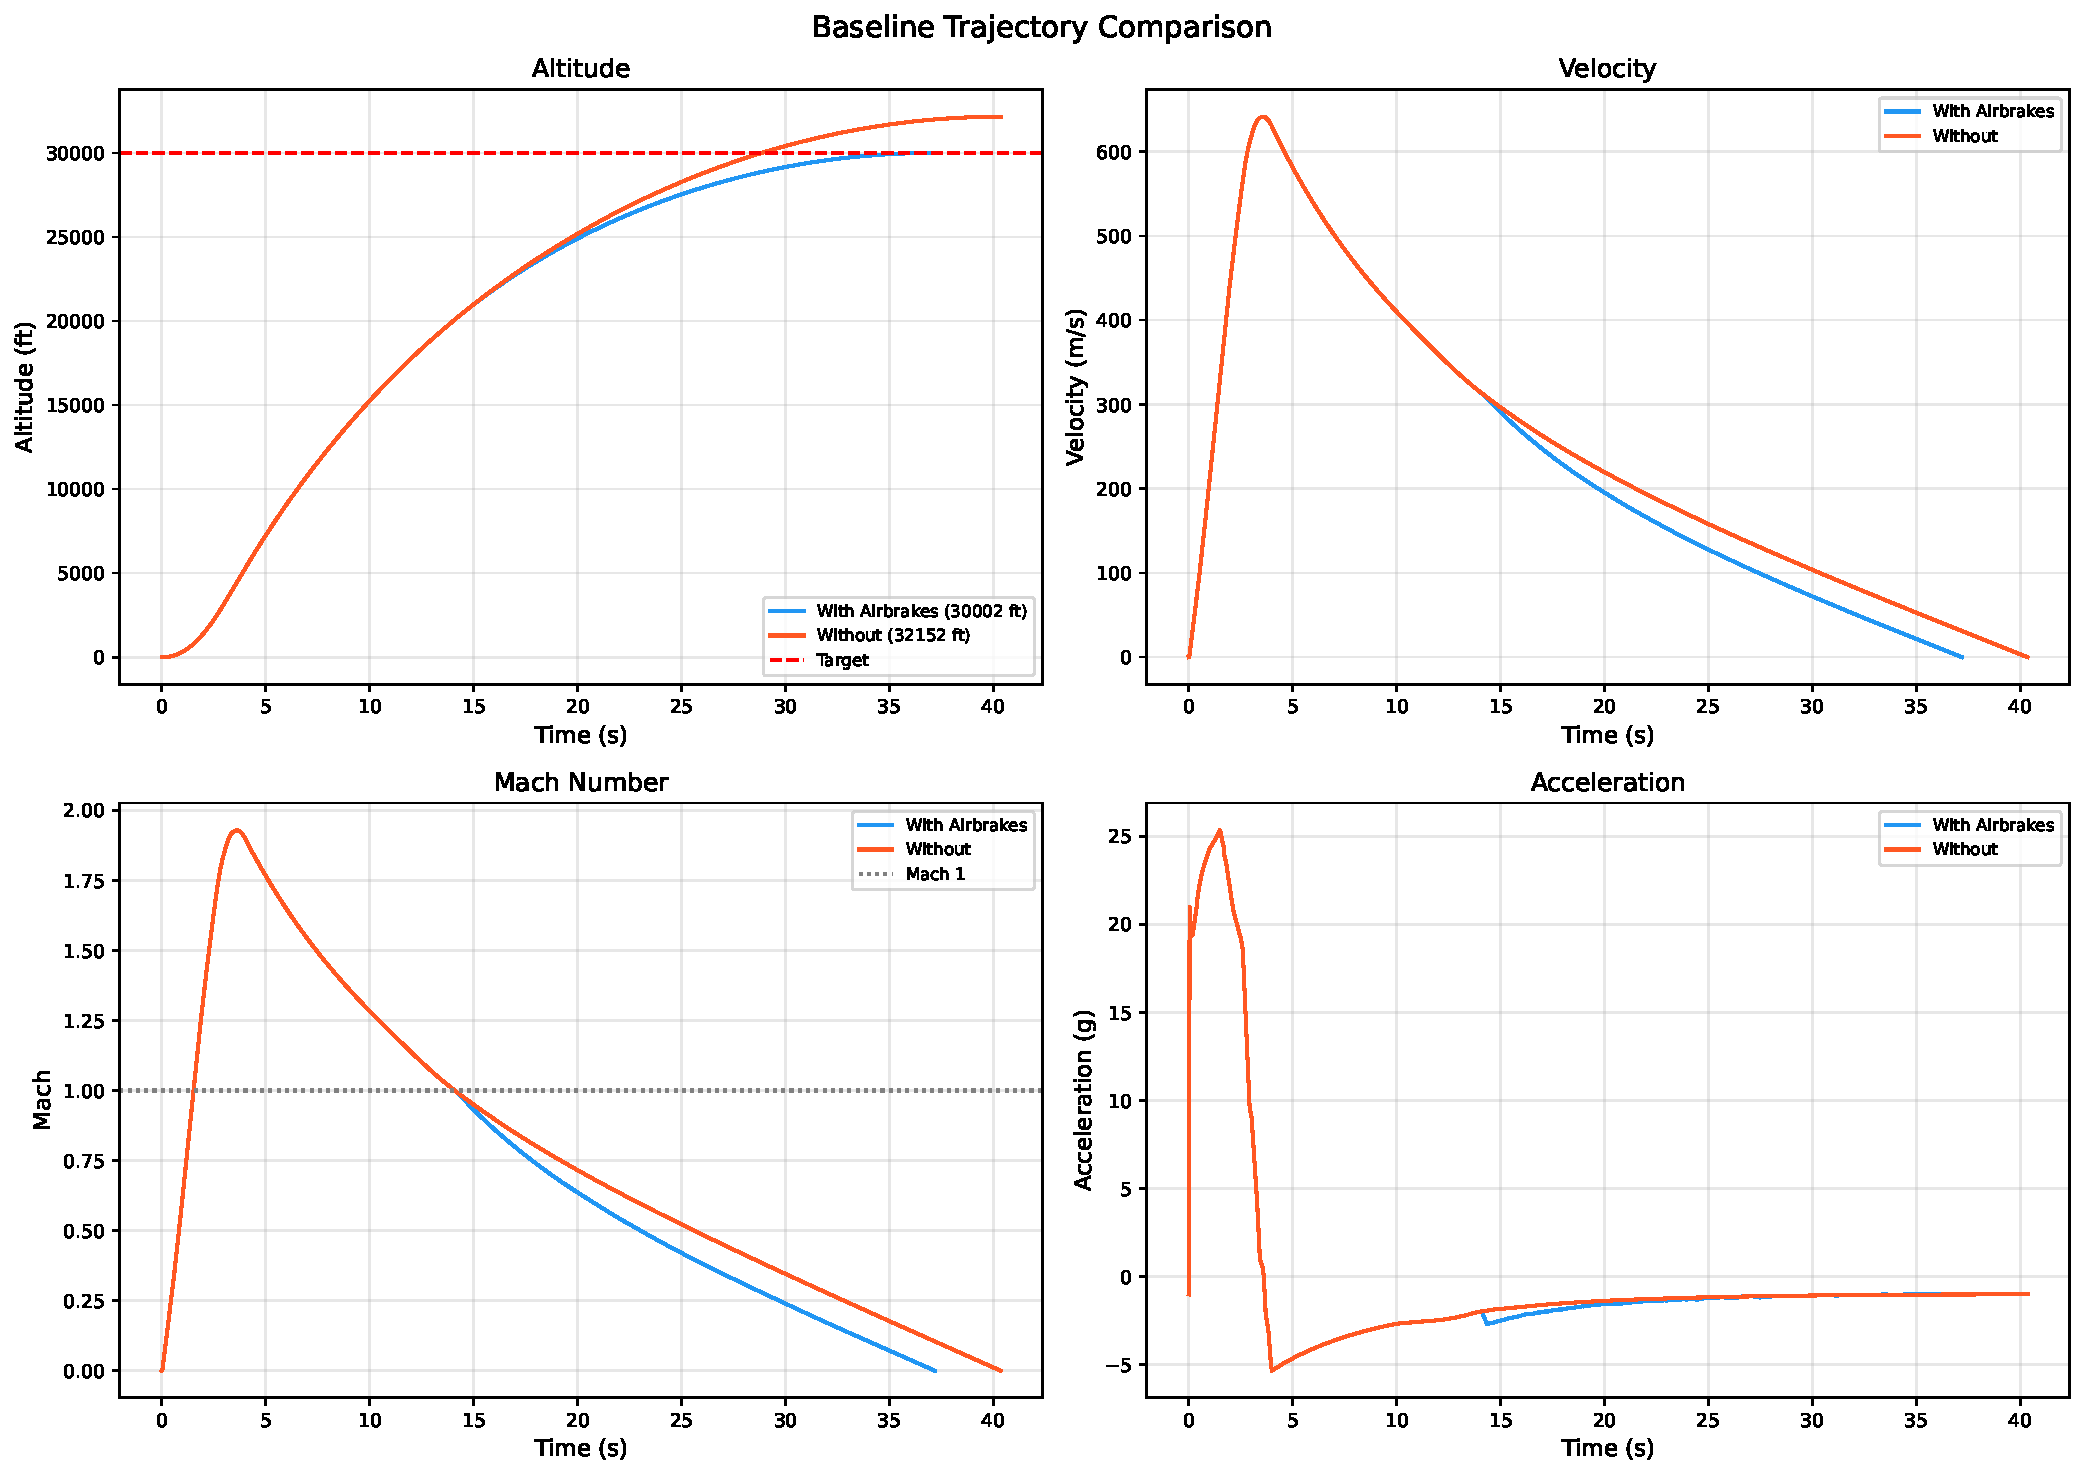
\includegraphics[width=0.92\textwidth]{S01_baseline_comparison.pdf}
    \caption{Baseline trajectory with and without airbrakes. The controlled flight hits \SI{30002}{\ft}; the uncontrolled flight overshoots to \SI{32152}{\ft}, confirming \SI{2150}{\ft} of available control authority.}
    \label{fig:baseline_comparison}
\end{figure}

The uncontrolled apogee of \SI{32152}{\ft} overshoots the target by \SI{2150}{\ft}. This margin is intentional: the rocket is designed with excess performance so the airbrakes have room to compensate for off-nominal conditions. With airbrakes active, the controller lands at \SI{30002}{\ft}---\SI{2}{\ft} from the target.

The vehicle reaches supersonic speeds during the burn, peaks near Mach~1.1, then decelerates through the transonic regime during early coast. The airbrakes cannot deploy until Mach drops below 1.0, which takes several seconds after burnout. Once they deploy, the higher deceleration rate is visible in the controlled velocity curve.


\subsection{Airbrake Effectiveness}
\label{sec:airbrake_effectiveness}

Figure~\ref{fig:airbrake_detail} provides a detailed view of the airbrake deployment and its effect on the trajectory during the coast phase.

\begin{figure}[H]
    \centering
    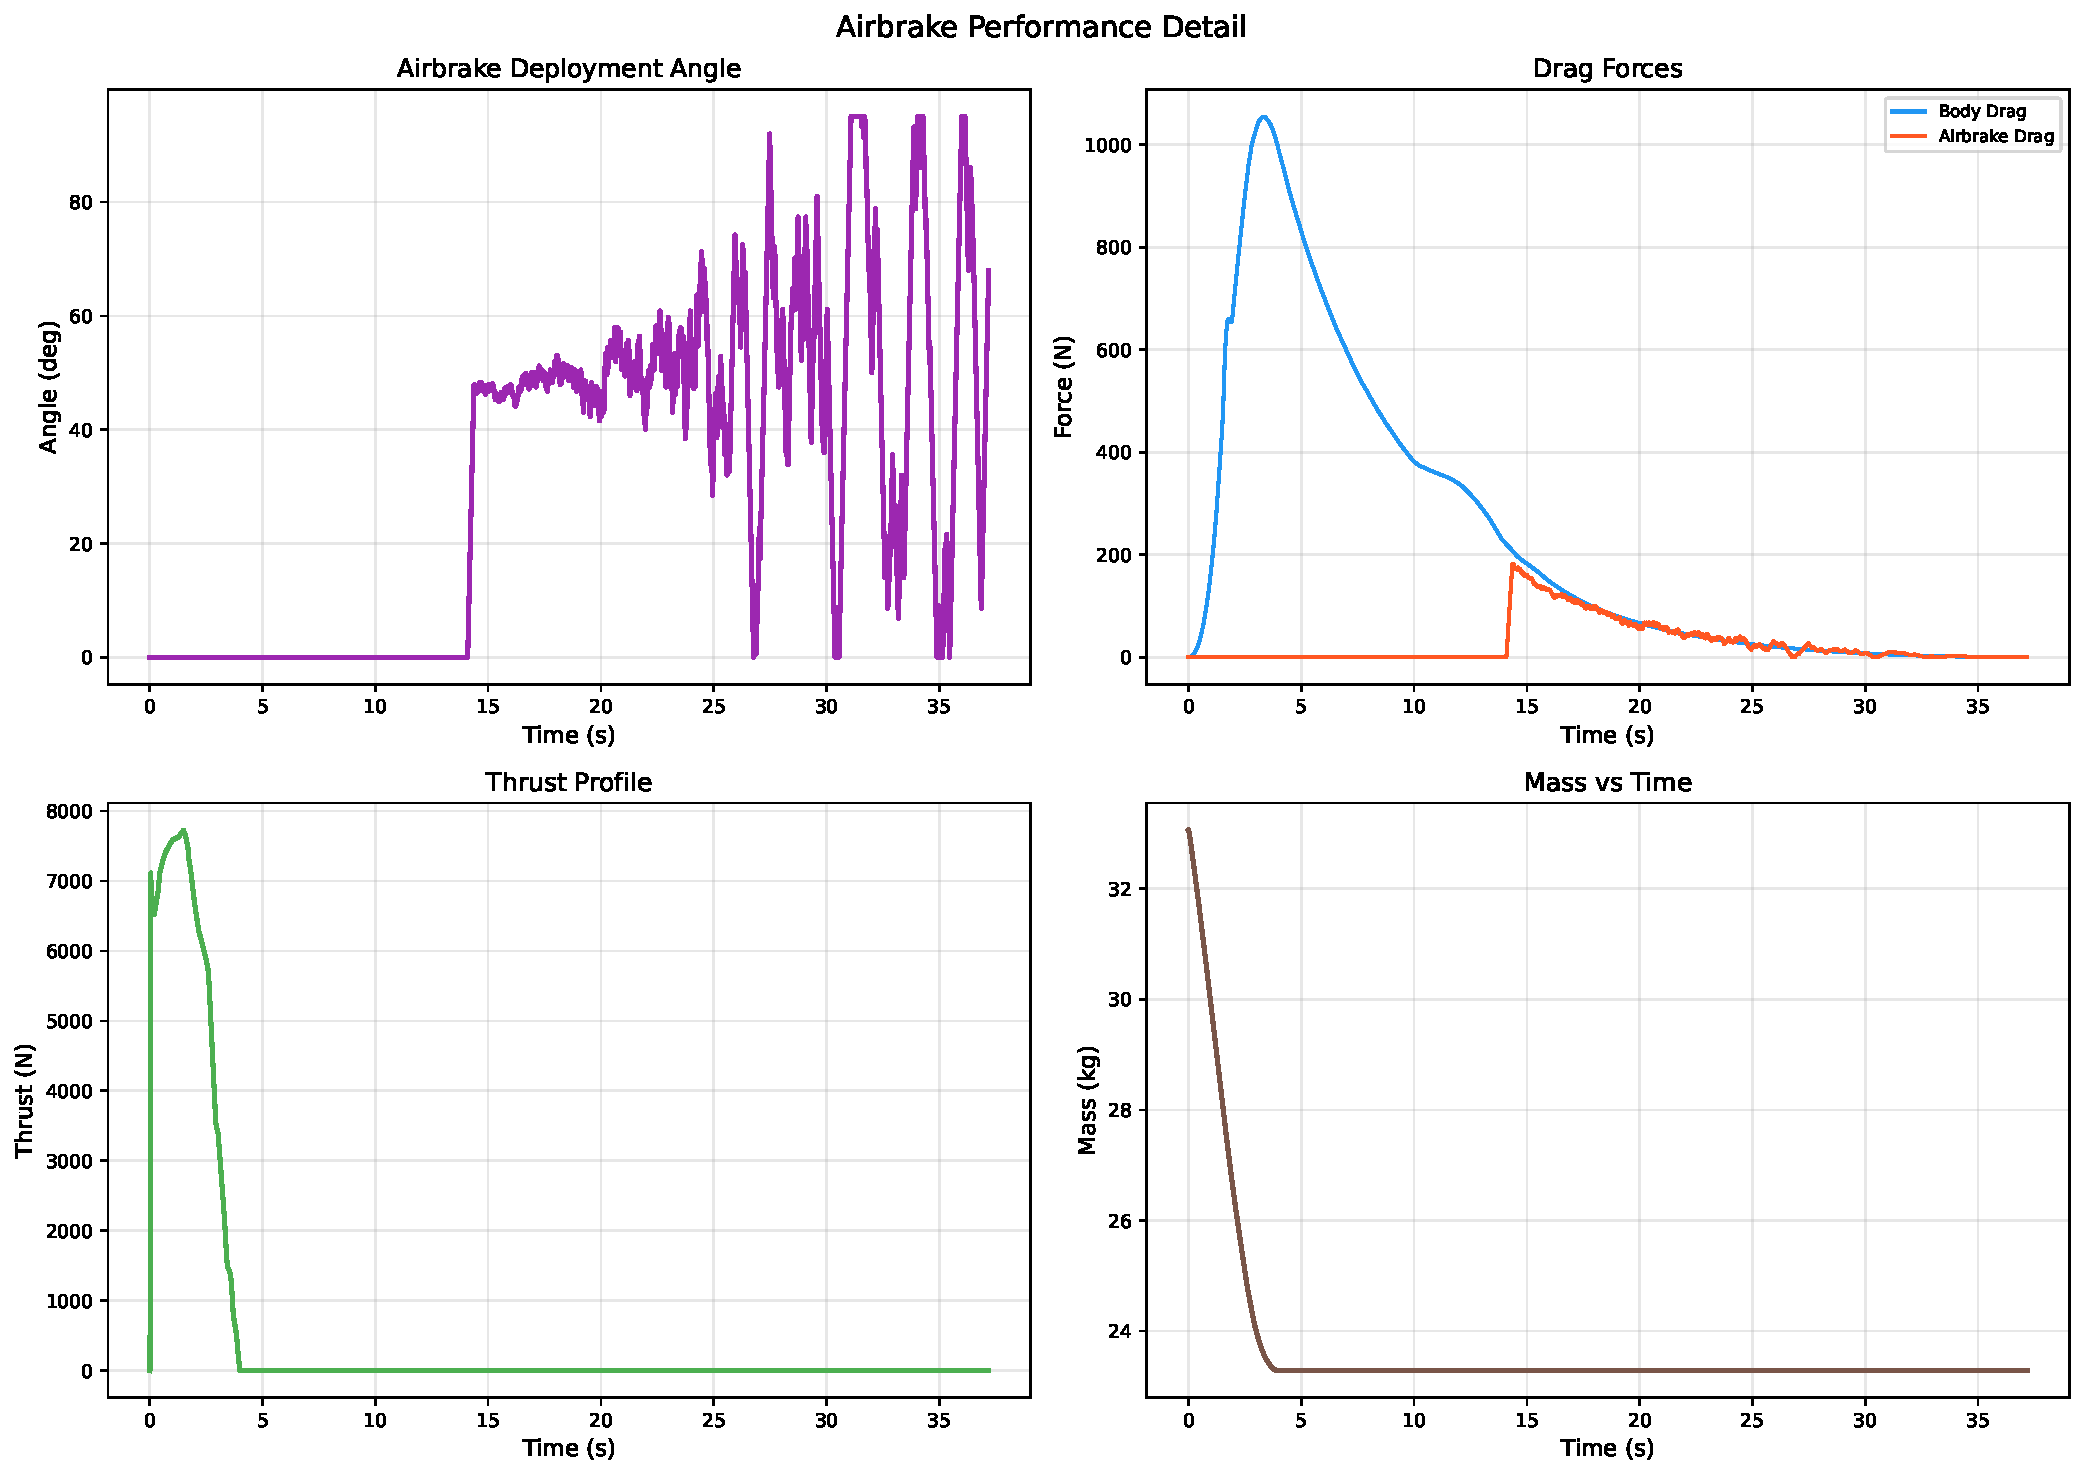
\includegraphics[width=0.92\textwidth]{S01_airbrake_detail.pdf}
    \caption{Airbrake deployment detail: deployment angle, drag forces (body vs.\ airbrake), thrust profile, and mass curve. Note the lockout period after burnout where airbrakes remain retracted until Mach~$<1.0$.}
    \label{fig:airbrake_detail}
\end{figure}

The deployment profile is not a step function---the controller modulates continuously, starting with a large deployment angle early in the coast (when velocity and thus braking authority are highest) and tapering off as the rocket approaches apogee. Drag scales as $v^2$, so most of the braking happens in the first few seconds after transonic lockout ends. By the time the vehicle nears apogee, even full deployment produces negligible drag. This front-loading is actually helpful: prediction errors late in the coast barely matter because there is almost no control authority left to misapply.


\subsection{Controller Behavior}
\label{sec:controller_behavior}

Figure~\ref{fig:controller_telemetry} shows the internal state of the controller during the flight, including the EKF state estimates, the predicted apogee, and the control authority bounds.

\begin{figure}[H]
    \centering
    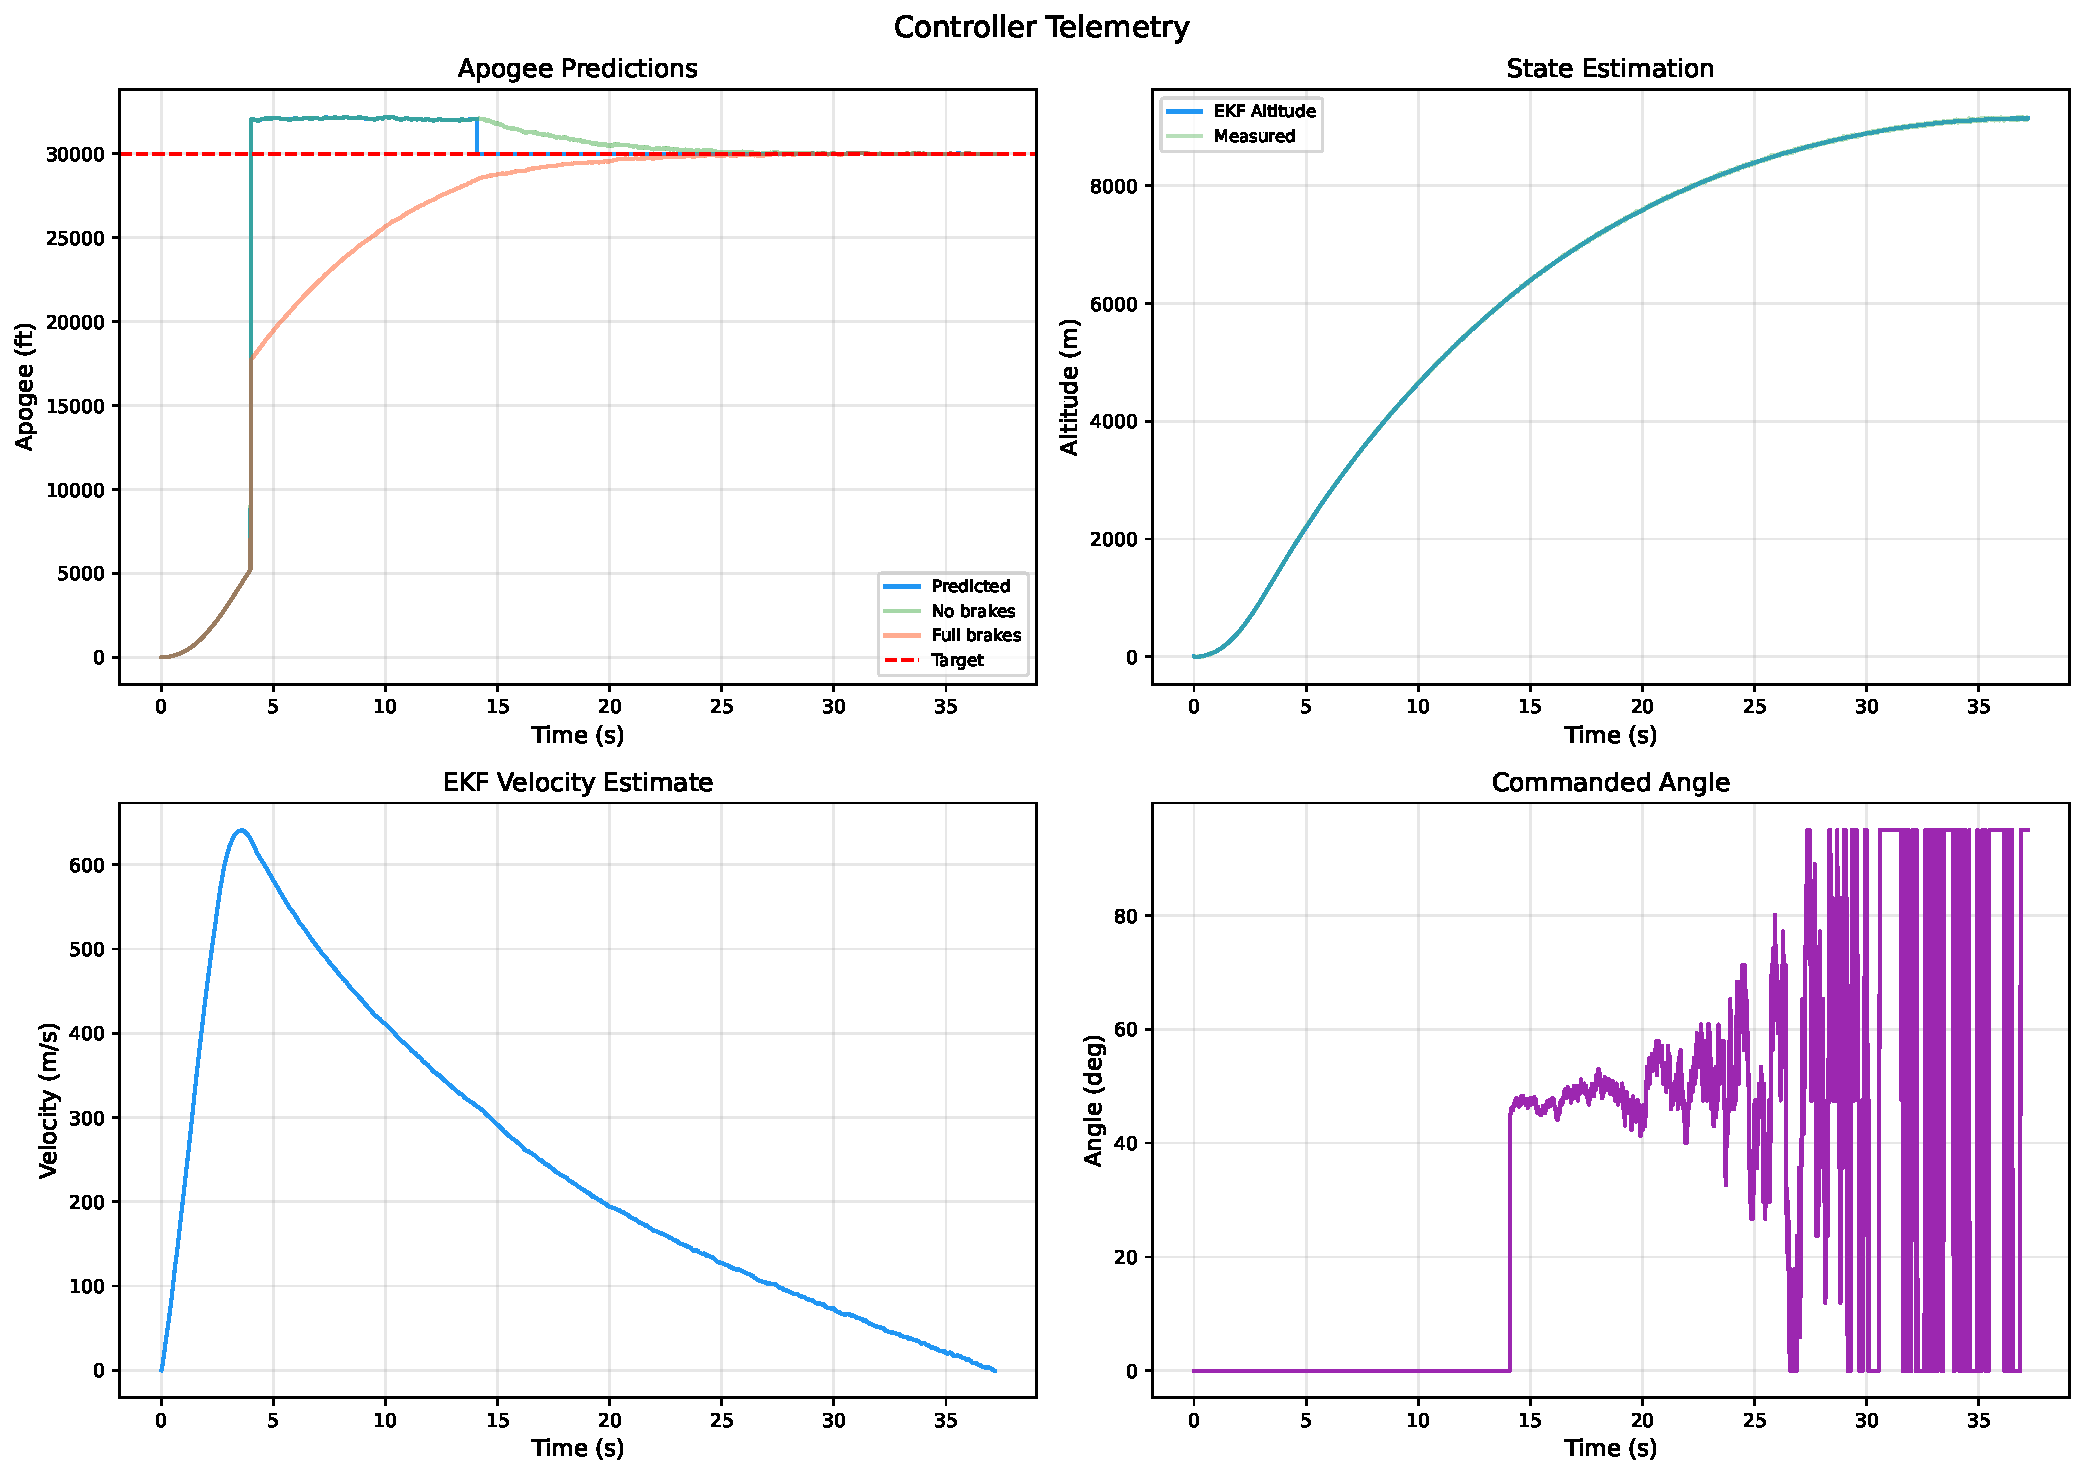
\includegraphics[width=0.92\textwidth]{S01_controller_telemetry.pdf}
    \caption{Controller telemetry: state estimates, apogee predictions (with no-brake and full-brake bounds), and commanded angle. The predicted apogee converges to the target within seconds of control activation; the authority envelope narrows as the vehicle decelerates.}
    \label{fig:controller_telemetry}
\end{figure}

Key observations from the telemetry:

\begin{enumerate}[nosep]
    \item \textbf{EKF accuracy:} Altitude and velocity estimates track truth closely. The filter converges in about 1--2 seconds after launch.

    \item \textbf{Apogee prediction convergence:} Once the controller enters the Active Coast phase, the predicted apogee rapidly converges toward the target altitude. The binary search typically requires only 5--7 iterations to converge within the \SI{1}{\metre} tolerance, which is well within the 10-iteration budget.

    \item \textbf{Control authority envelope:} The shaded region between the clean (no-brake) and full-brake apogee predictions represents the controller's instantaneous control authority. This envelope is widest immediately after the transonic lockout (when the vehicle has the most remaining kinetic energy) and narrows as the vehicle decelerates. The target altitude must lie within this envelope for the controller to achieve its objective; if the clean apogee is already below the target, the airbrakes cannot help (the rocket is already undershooting).

    \item \textbf{State machine transitions:} The controller correctly transitions through Boost, Transonic Lockout, Active Coast (with sub-states for modulation, undershooting, and max braking), and Recovery phases. The transitions are smooth, with no oscillation or chattering between states.
\end{enumerate}

With the baseline established at $+2$~ft error, the following sections perturb each parameter to map where performance starts to degrade.


% AERODYNAMIC UNCERTAINTY STUDY
\section{Aerodynamic Uncertainty Study}
\label{sec:aero_uncertainty}

For a student rocket without wind tunnel data, the drag coefficient is the least well-known parameter in the trajectory model. Our $\Cd(M)$ curve comes from semi-empirical tools, and the true uncertainty could easily be 5--20\% depending on how accurately the geometry, surface finish, and protuberances are captured.

We ran 1{,}000 Monte Carlo trajectories at each of three $\Cd$ uncertainty levels (5\%, 10\%, 15\%), perturbing the simulation model's body drag coefficient while leaving the controller's internal $\Cd$ model unchanged. For each run, two independent Gaussian scale factors are drawn at Mach~0 and Mach~2:
\begin{align}
    s_{\mathrm{low}} &\sim \mathcal{N}(1.0, \sigma_{\Cd}^2), \label{eq:cd_scale_low} \\
    s_{\mathrm{high}} &\sim \mathcal{N}(1.0, \sigma_{\Cd}^2), \label{eq:cd_scale_high}
\end{align}
and linearly interpolated across Mach number:
\begin{equation}
    s(M) = s_{\mathrm{low}} + \frac{M}{2.0} (s_{\mathrm{high}} - s_{\mathrm{low}}).
    \label{eq:cd_scale_interp}
\end{equation}
The simulation $\Cd$ is then $\Cd^{\mathrm{sim}}(M) = s(M) \cdot \Cd^{\mathrm{truth}}(M)$. Each run also includes default sensor noise with a random multiplier drawn from $\mathcal{N}(1.0, 0.2^2)$.

\subsection{Results}
\label{sec:aero_results}

The results across all three uncertainty levels are summarized below and compared in Figure~\ref{fig:cd_boxplot}. At 5\% $\Cd$ uncertainty: mean = 30{,}034~ft, $\sigma = 158$~ft, 97.6\% within $\pm$500~ft. At 10\%: mean = 30{,}204~ft, $\sigma = 786$~ft, 79.2\%. At 15\%: mean = 30{,}404~ft, $\sigma = 1{,}645$~ft, 61.3\%. The distributions are approximately Gaussian, centered near the target at all levels, with standard deviation scaling roughly linearly with the $\Cd$ perturbation magnitude. A notable asymmetry appears at higher uncertainty levels: runs where the true $\Cd$ is lower than modeled (less drag than expected) produce larger overshoots than the corresponding undershoots from high-$\Cd$ runs. This occurs because a lower-than-expected $\Cd$ means the rocket carries more kinetic energy into the coast phase, and the airbrakes may be insufficient to dissipate the excess.

\subsubsection{Cross-Case Comparison}

Figure~\ref{fig:cd_boxplot} provides a box-and-whisker comparison across all three uncertainty levels.

\begin{figure}[H]
    \centering
    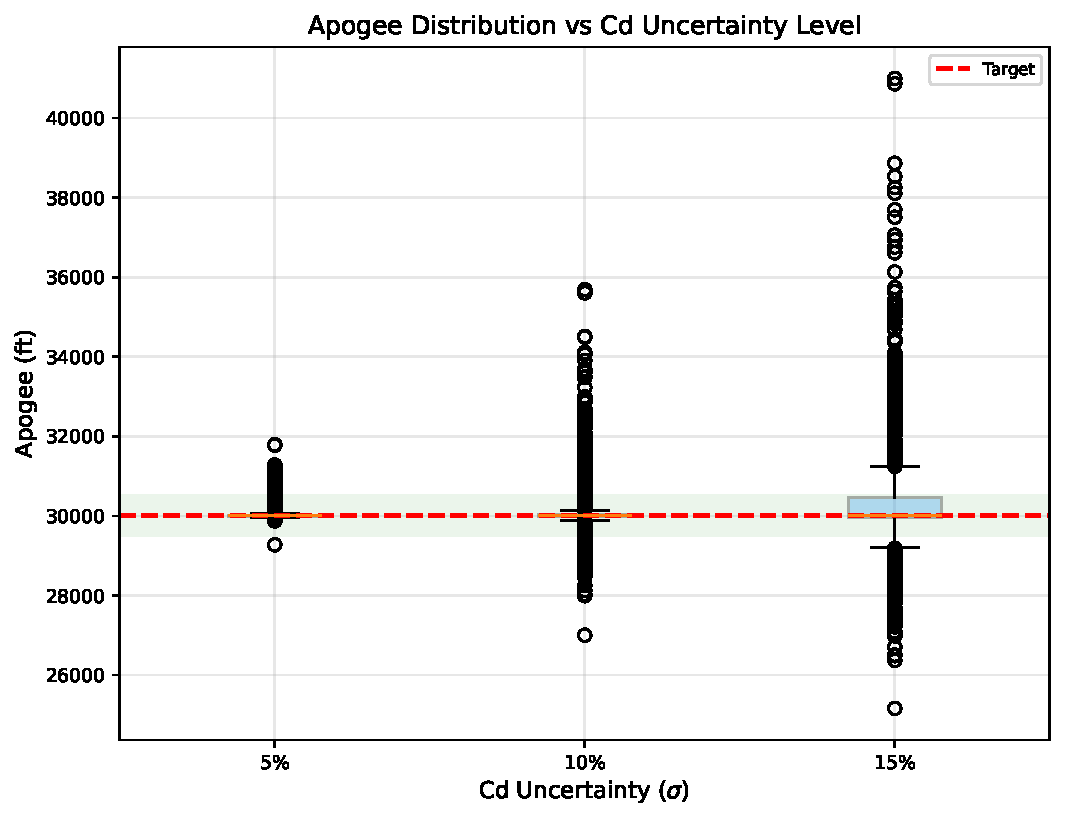
\includegraphics[width=0.85\textwidth]{S02_cd_boxplot.pdf}
    \caption{Box-and-whisker plot comparing apogee distributions across the three $\Cd$ uncertainty levels (5\%, 10\%, 15\%). The boxes show the interquartile range (25th to 75th percentile), the horizontal line is the median, and the whiskers extend to the 5th and 95th percentiles. The progressive increase in spread with uncertainty level is clearly visible, while the median remains close to the target in all cases.}
    \label{fig:cd_boxplot}
\end{figure}


\subsection{Discussion}
\label{sec:aero_discussion}

Implications for hardware and mission planning:

\begin{enumerate}[nosep]
    \item \textbf{Controller robustness:} The feed-forward controller with binary search maintains accurate mean apogee targeting across all tested uncertainty levels. Even at 15\% $\Cd$ uncertainty, the mean error is small compared to the distribution width, indicating that the controller does not exhibit systematic bias under model mismatch.

    \item \textbf{Asymmetric sensitivity:} The controller is more sensitive to $\Cd$ underestimates (true drag lower than modeled) than overestimates. This is physically intuitive: when the real drag is lower, the rocket carries more energy than the controller expects, and the airbrakes must compensate for the ``extra'' energy. Conversely, when the real drag is higher, the rocket naturally decelerates faster than predicted, and the controller simply reduces airbrake deployment. This asymmetry has design implications: it is better to err on the side of slightly overestimating drag in the model, as the controller handles overestimates more easily.

    \item \textbf{Mach-dependent effects:} Because the $\Cd$ perturbation varies with Mach number, runs where the error is concentrated in the subsonic regime (where the airbrakes operate) produce larger apogee deviations than runs where the error is primarily in the transonic/supersonic regime (where the airbrakes are locked out). This suggests that improving the accuracy of the subsonic $\Cd$ prediction is more valuable than refining the transonic drag rise for the purposes of airbrake control.

    \item \textbf{Scaling for design margins:} The approximately linear relationship between $\sigma_{\Cd}$ and $\sigma_{\mathrm{apogee}}$ allows interpolation for design margin calculations. For a competition scoring window of $\pm$\SI{500}{\ft}, the controller achieves high success rates even at 10\% $\Cd$ uncertainty.
\end{enumerate}

Wind tunnel testing or CFD to bring $\sigma_{\Cd}$ below 10\% would pay off roughly proportionally in apogee accuracy.


% MOTOR THRUST DISPERSION
\section{Motor Thrust Dispersion}
\label{sec:thrust}

Commercial solid rocket motors exhibit manufacturing-induced variability in total impulse and thrust profile. Motor-to-motor performance dispersion arises from variations in propellant composition, grain geometry, nozzle erosion characteristics, and ambient temperature effects on burn rate. Published data from motor manufacturers typically quote total impulse variability on the order of 2--5\% ($1\sigma$) for certified motors.

We ran 1{,}000 Monte Carlo trajectories at each of three thrust dispersion levels (2\%, 3\%, 5\%), applying a global scaling factor $s_T \sim \mathcal{N}(1.0, \sigma_T^2)$ to the thrust-time curve:
\begin{equation}
    T^{\mathrm{sim}}(t) = s_T \cdot T^{\mathrm{truth}}(t).
    \label{eq:thrust_scale}
\end{equation}
The $\Cd$ model is held at nominal values, isolating the effect of thrust variability. Default sensor noise with a random multiplier is applied to each run.

\subsection{Results}
\label{sec:thrust_results}

At 2\% thrust dispersion: mean = 30{,}041~ft, $\sigma = 176$~ft, 96.3\% within $\pm$500~ft. At 3\%: mean = 30{,}108~ft, $\sigma = 470$~ft, 85.8\%. At 5\%: mean = 30{,}216~ft, $\sigma = 1{,}229$~ft, 64.7\%. The controller compensates effectively at all levels, with the distribution broadening progressively but the mean remaining close to the target. A 5\% thrust dispersion produces comparable apogee scatter to a 10\% $\Cd$ uncertainty, suggesting that $\Cd$ has roughly twice the impact per unit standard deviation.

\subsubsection{Cross-Case Comparison}

\begin{figure}[H]
    \centering
    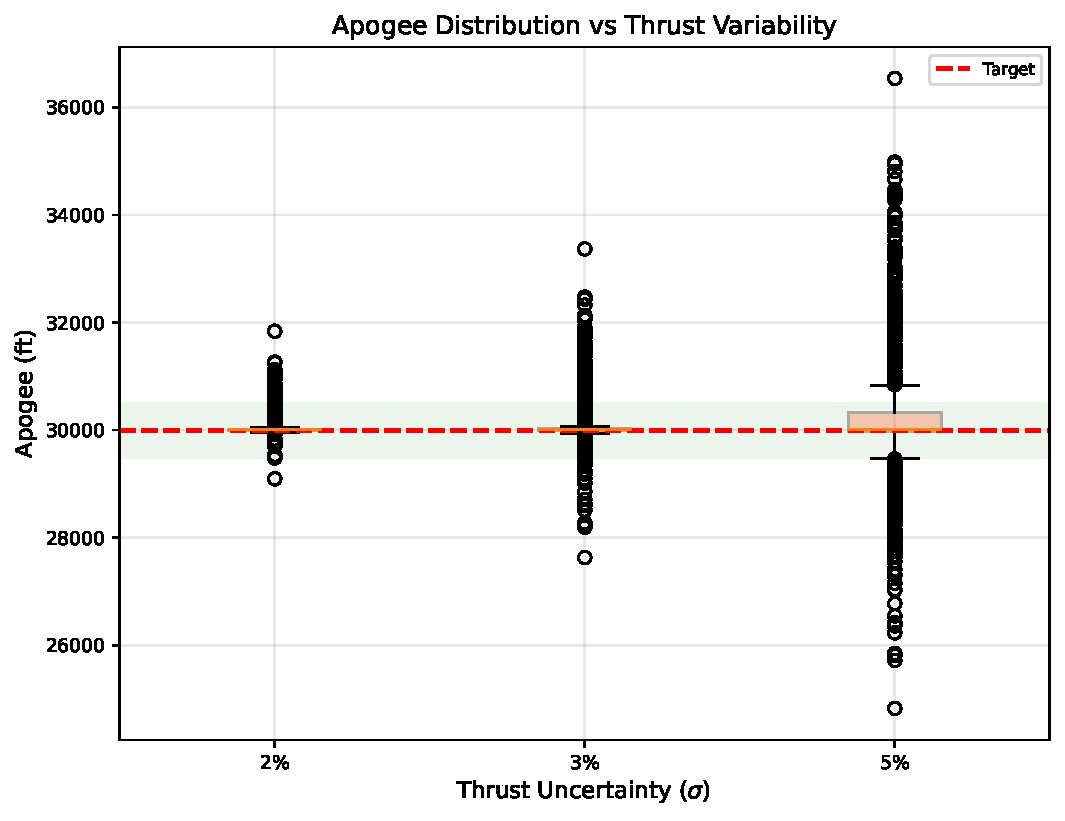
\includegraphics[width=0.85\textwidth]{S03_thrust_boxplot.pdf}
    \caption{Box-and-whisker plot comparing apogee distributions across the three thrust dispersion levels (2\%, 3\%, 5\%). As with the aerodynamic study, the spread increases progressively with uncertainty level while the median remains near the target.}
    \label{fig:thrust_boxplot}
\end{figure}

\begin{figure}[H]
    \centering
    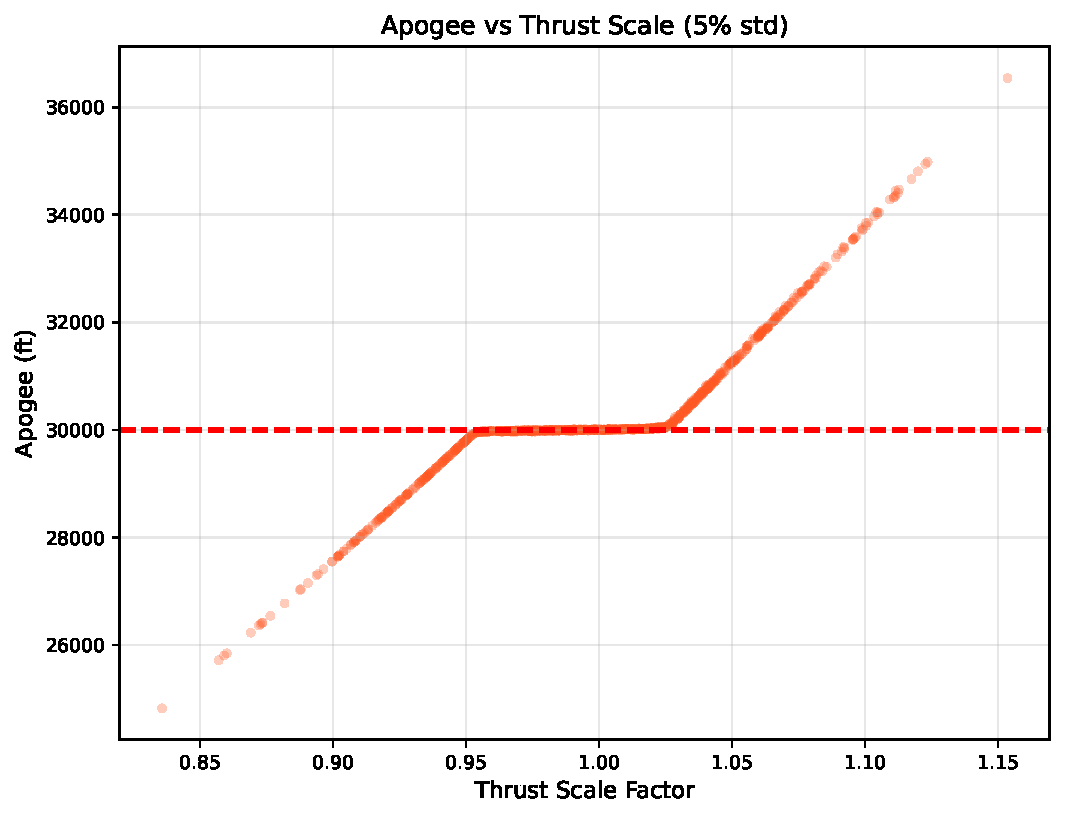
\includegraphics[width=0.85\textwidth]{S03_thrust_scatter.pdf}
    \caption{Scatter plot of achieved apogee versus thrust scale factor for the 5\% dispersion study. The strong linear correlation demonstrates the direct relationship between total impulse and uncontrolled apogee, with the controller partially but not completely compensating for the thrust variation.}
    \label{fig:thrust_scatter}
\end{figure}

Figure~\ref{fig:thrust_scatter} reveals the mechanism by which thrust dispersion affects the controlled apogee. Higher thrust factors produce higher burnout velocities and altitudes, giving the vehicle more total energy. The controller attempts to compensate by deploying more airbrake area, but because the $\Cd$ model is correct in this study (only thrust is perturbed), the compensation is quite effective. The residual apogee error is primarily due to the controller's inability to perfectly predict the trajectory with its coarsened internal model and noisy sensor inputs.


\subsection{Discussion}
\label{sec:thrust_discussion}

Key takeaways from the thrust study:

\begin{enumerate}[nosep]
    \item \textbf{Effective compensation:} The feed-forward controller effectively compensates for thrust variability because thrust perturbations manifest as different burnout conditions (velocity and altitude), which are directly observable by the EKF. Unlike $\Cd$ errors, which create a persistent mismatch between the controller's drag model and reality throughout the coast phase, thrust errors create a one-time offset in initial conditions that the controller can sense and adapt to.

    \item \textbf{Near-symmetric response:} The apogee distribution under thrust perturbation is more symmetric than under $\Cd$ perturbation. High thrust produces higher burnout conditions, requiring more airbrake deployment, while low thrust produces the opposite. The controller handles both directions equally well because the control authority (airbrake deployment range) is symmetric.

    \item \textbf{Comparison to $\Cd$ uncertainty:} A 5\% thrust dispersion produces comparable scatter to a 10\% $\Cd$ uncertainty. The difference in leverage makes sense: $\Cd$ errors accumulate over the entire coast, while thrust errors only affect burnout conditions.

    \item \textbf{Motor selection implications:} For competition purposes, selecting a motor with well-characterized and consistent performance (low lot-to-lot variability) provides tangible benefits, but the controller's compensation ability means that the additional cost of premium motors may not be justified if the $\Cd$ uncertainty budget is already the dominant error source.
\end{enumerate}


% WIND PERTURBATION STUDY
\section{Wind Perturbation Study}
\label{sec:wind}

Wind is a ubiquitous source of uncertainty in outdoor rocketry. While horizontal winds primarily cause weathercocking and trajectory tilting, the vertical component of the wind field directly affects the effective aerodynamic velocity seen by the rocket and thus the drag force magnitude. This study isolates the effect of random vertical wind perturbations on controlled apogee accuracy.

We ran 1{,}000 Monte Carlo trajectories at each of four vertical wind levels ($\sigma_w \in \{1, 2, 3, 5\}$~m/s), drawing a constant vertical wind $w \sim \mathcal{N}(0, \sigma_w^2)$ for each run:
\begin{equation}
    w \sim \mathcal{N}(0, \sigma_w^2).
    \label{eq:wind_model}
\end{equation}
The wind modifies the effective vertical velocity used in drag calculations. The controller does not have direct wind speed information---it infers the wind effect from the trajectory deviation observed through the EKF.

\subsection{Results}
\label{sec:wind_results}

The wind perturbation results show very small sensitivity across all tested levels. At $\sigma_w = 1$~m/s: mean = 30{,}004~ft, $\sigma = 9$~ft, 100\% within $\pm$500~ft. At 3~m/s: mean = 30{,}008~ft, $\sigma = 23$~ft, 100\%. At 5~m/s: mean = 30{,}020~ft, $\sigma = 67$~ft, 99.6\%. Even at the strongest wind level, the apogee scatter is an order of magnitude smaller than the $\Cd$ or thrust studies. Figure~\ref{fig:wind_boxplot} confirms the modest sensitivity.

\begin{figure}[H]
    \centering
    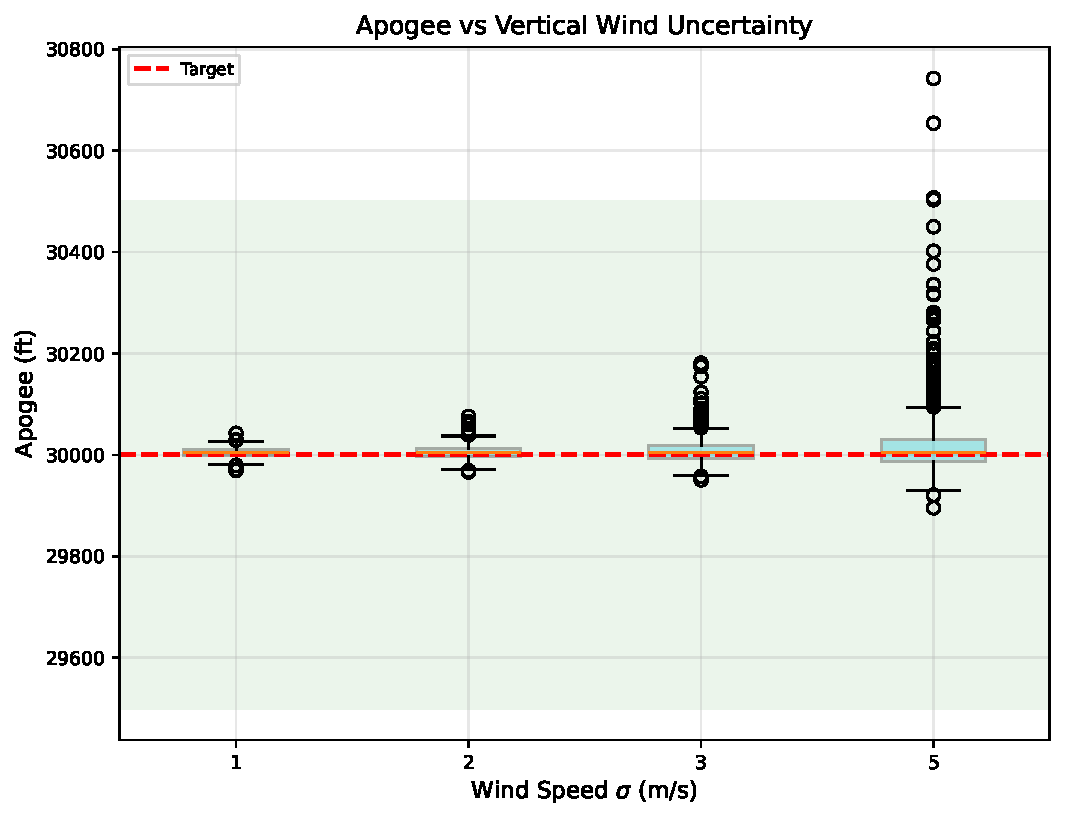
\includegraphics[width=0.85\textwidth]{S04_wind_boxplot.pdf}
    \caption{Box-and-whisker plot comparing apogee distributions across all four wind perturbation levels. The very modest increase in spread from \SI{1}{\metre\per\second} to \SI{5}{\metre\per\second} demonstrates that vertical wind perturbations are a secondary contributor to apogee uncertainty compared to aerodynamic coefficient and thrust errors.}
    \label{fig:wind_boxplot}
\end{figure}

The physical explanation lies in the relative magnitudes involved. During the coast phase, the rocket's vertical velocity ranges from approximately 300~m/s at the start of active control down to 0~m/s at apogee. A vertical wind component of even \SI{5}{\metre\per\second} represents less than 2\% of the vehicle's velocity for most of the control-active period. Since drag scales as $v^2$, the wind-induced change in drag force is on the order of $2 \times (w/v) \approx 3\%$ at most, and this fractional change diminishes as the vehicle decelerates. Teams need not invest disproportionate effort in vertical wind prediction or compensation algorithms. However, this study considers only the vertical wind component; horizontal winds can induce trajectory tilting that effectively reduces the altitude gained per unit energy, an effect not captured by this one-dimensional simulation.


% COMBINED UNCERTAINTY ANALYSIS
\section{Combined Uncertainty Analysis}
\label{sec:combined}

\subsection{Joint Parameter Distribution}
\label{sec:combined_distribution}

The combined uncertainty study simultaneously perturbs the following parameters for each of 1{,}000 Monte Carlo runs:

\begin{table}[H]
\centering
\caption{Combined uncertainty study parameter distributions.}
\label{tab:combined_params}
\begin{tabular}{@{}llc@{}}
\toprule
\textbf{Parameter} & \textbf{Distribution} & \textbf{Value} \\
\midrule
Body $\Cd$ scale (Mach 0) & $\mathcal{N}(1.0, \sigma^2)$ & $\sigma = 0.10$ (10\%) \\
Body $\Cd$ scale (Mach 2) & $\mathcal{N}(1.0, \sigma^2)$ & $\sigma = 0.10$ (10\%) \\
Airbrake $\Cd$ scale (Mach 0) & $\mathcal{N}(1.0, \sigma^2)$ & $\sigma = 0.05$ (5\%) \\
Airbrake $\Cd$ scale (Mach 2) & $\mathcal{N}(1.0, \sigma^2)$ & $\sigma = 0.05$ (5\%) \\
Thrust scale & $\mathcal{N}(1.0, \sigma^2)$ & $\sigma = 0.03$ (3\%) \\
Temperature offset & $\mathcal{N}(0, \sigma^2)$ & $\sigma = \SI{10}{\kelvin}$ \\
Sensor noise multiplier & $\mathcal{N}(1.0, \sigma^2)$ & $\sigma = 0.20$ \\
\bottomrule
\end{tabular}
\end{table}

This parameter set represents our best estimate of the joint uncertainty faced during an actual IREC launch. The 10\% $\Cd$ uncertainty represents a moderately well-characterized vehicle, the 3\% thrust dispersion is typical for certified commercial motors, the \SI{10}{\kelvin} temperature offset captures non-standard day conditions ), and the sensor noise multiplier accounts for unit-to-unit variability in sensor performance.

All parameters are drawn independently---we do not model correlations between, for example, $\Cd$ and thrust. This is a reasonable simplification since the physical mechanisms driving aerodynamic uncertainty (geometry, surface finish) are largely independent of motor performance (propellant chemistry, grain geometry).

\subsection{Results}
\label{sec:combined_results}

\begin{figure}[H]
    \centering
    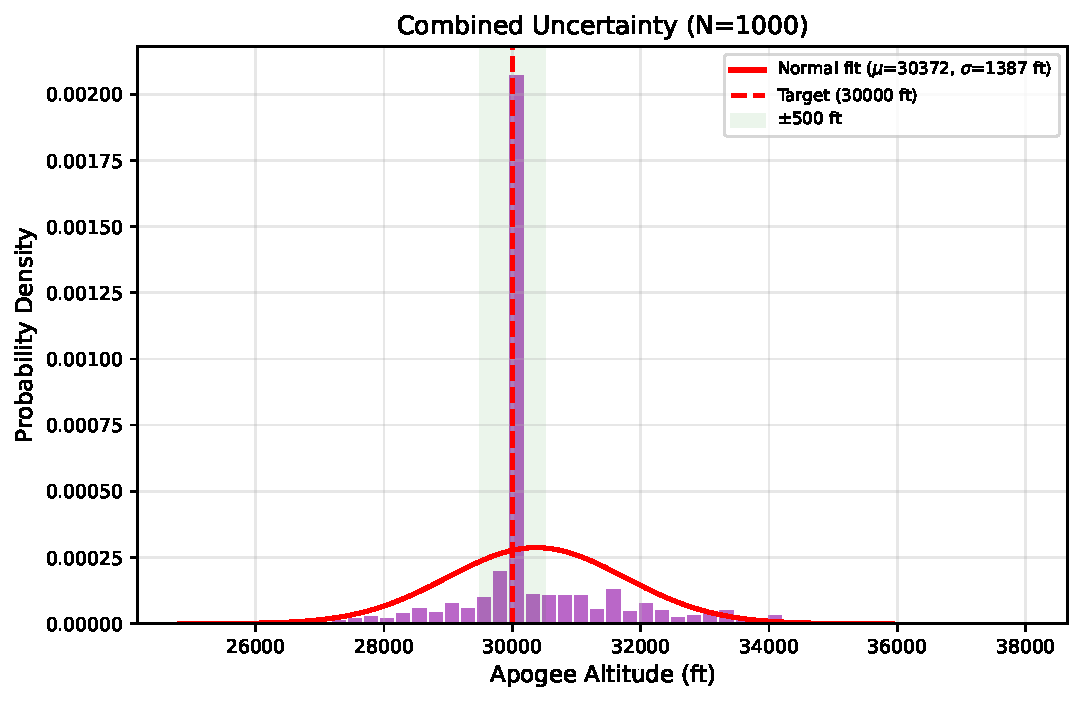
\includegraphics[width=0.85\textwidth]{S05_combined_hist.pdf}
    \caption{Apogee altitude histogram for 1{,}000 Monte Carlo runs with combined uncertainty (10\% $\Cd$ + 3\% thrust + \SI{10}{\kelvin} temperature + sensor noise). The distribution is wider than any single-source study at comparable levels, reflecting the compounding of multiple uncertainty sources.}
    \label{fig:combined_hist}
\end{figure}

The combined uncertainty study produces the widest apogee distribution of all the studies presented so far. The standard deviation is larger than any single-source study, confirming that the uncertainties compound when applied simultaneously. However, the increase is sub-additive: the combined standard deviation is less than the root-sum-square of the individual standard deviations, suggesting that some of the uncertainty sources partially cancel (e.g., a high-$\Cd$ run with high thrust may approximately balance out).

\subsection{Dominant Uncertainty Sources}
\label{sec:combined_dominant}

\begin{figure}[H]
    \centering
    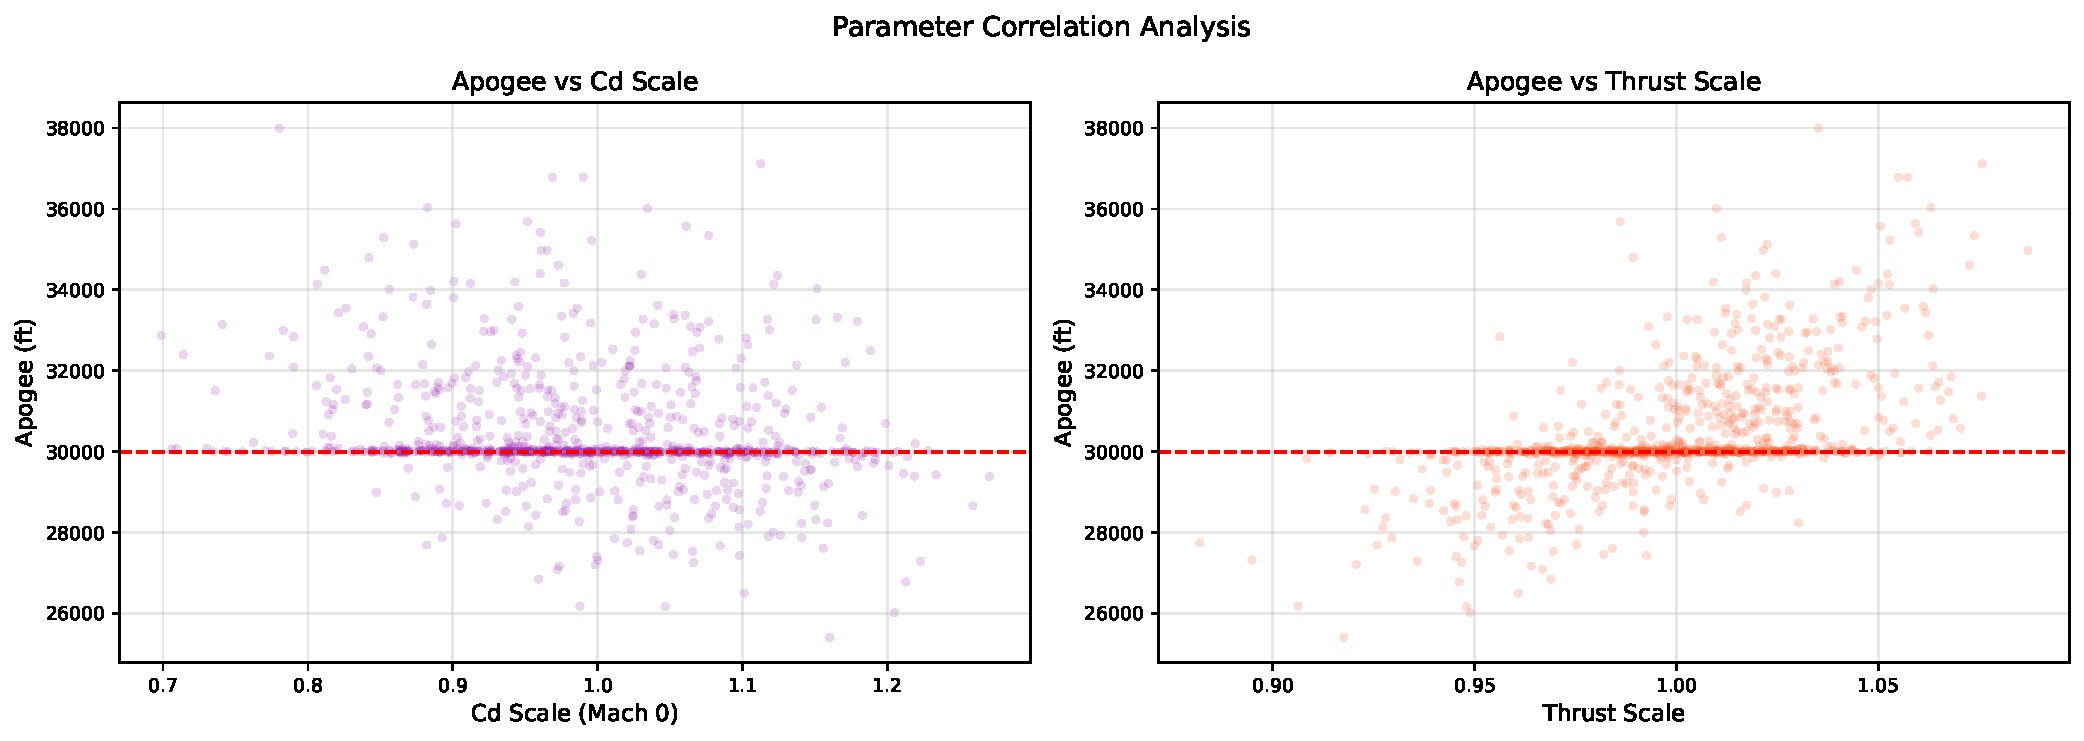
\includegraphics[width=0.85\textwidth]{S05_combined_correlation.pdf}
    \caption{Correlation matrix showing the relationship between input parameter variations and achieved apogee for the combined uncertainty study. The strongest correlations identify the dominant uncertainty sources. $\Cd$ scale factors show the largest correlation magnitude, followed by thrust scale, with temperature and sensor noise showing the weakest correlations.}
    \label{fig:combined_correlation}
\end{figure}

Figure~\ref{fig:combined_correlation} presents the correlation structure between the randomized input parameters and the achieved apogee. The analysis reveals a clear hierarchy of uncertainty importance:

\begin{enumerate}[nosep]
    \item \textbf{Body $\Cd$ uncertainty (dominant):} The body drag coefficient scale factors show the strongest correlation with apogee error, confirming the findings from Section~\ref{sec:aero_uncertainty}. The low-Mach $\Cd$ scale has a stronger correlation than the high-Mach scale because the airbrakes operate primarily in the subsonic regime.

    \item \textbf{Motor thrust dispersion (secondary):} The thrust scale factor shows a moderate positive correlation with apogee---higher thrust leads to higher apogee, partially compensated by the controller. This is the second-most important uncertainty source.

    \item \textbf{Airbrake $\Cd$ uncertainty (tertiary):} Uncertainty in the airbrake drag coefficient has a smaller but non-negligible effect. Errors in the airbrake $\Cd$ directly affect the controller's ability to predict the braking effect of a given deployment angle.

    \item \textbf{Temperature offset (minor):} Non-standard atmospheric temperature has a small effect through its influence on air density and speed of sound. A warmer-than-standard day reduces density, decreasing both body drag and airbrake effectiveness, leading to slightly higher apogees.

    \item \textbf{Sensor noise (negligible):} The noise multiplier shows near-zero correlation with apogee. The EKF averages out random noise well enough that sensor quality barely matters for apogee accuracy.
\end{enumerate}

This hierarchy provides a clear prioritization for engineering effort. Resources should be allocated first to improving aerodynamic characterization (reducing $\sigma_{\Cd}$), then to motor performance consistency (selecting well-characterized motors or conducting static test firings), with relatively little benefit from improving sensor quality or atmospheric modeling beyond the baseline levels.

The combined study also serves as the best available prediction of actual flight performance. The 90\% confidence interval (5th to 95th percentile) represents the range within which we expect the flight-day apogee to fall with 90\% probability, assuming the uncertainty budgets are correctly characterized. This interval should be communicated to competition officials and used for safety margin calculations.

% SENSOR PERFORMANCE ANALYSIS
\section{Sensor Performance Analysis}
\label{sec:sensor}

We test three sensor failure modes: noise amplification, static bias, and complete sensor loss.

\subsection{Noise Sensitivity Analysis}
\label{sec:noise_sensitivity}

We swept the sensor noise multiplier $k_n \in \{0.25, 0.5, 1.0, 2.0, 5.0, 10.0, 15.0, 20.0, 25.0\}$ (scaling all three channels simultaneously), running 1{,}000 Monte Carlo trajectories at each level with all other parameters held at nominal. At $k_n = 0.25$, the noise levels are $\sigma_p = \SI{12.5}{\pascal}$, $\sigma_a = \SI{0.125}{\metre\per\second\squared}$, $\sigma_T = \SI{0.125}{\kelvin}$; at $k_n = 25$, they reach $\sigma_p = \SI{1250}{\pascal}$, $\sigma_a = \SI{12.5}{\metre\per\second\squared}$, $\sigma_T = \SI{12.5}{\kelvin}$.

\subsubsection{EKF Noise Rejection Mechanism}

The EKF's ability to reject measurement noise stems from the Kalman gain computation, which optimally blends the process model prediction with the noisy measurements. For a scalar measurement with noise variance $R$ and prior state uncertainty $P^{-}$, the Kalman gain is:
\begin{equation}
    K = \frac{P^{-} H^T}{H P^{-} H^T + R}
    \label{eq:kalman_gain_noise}
\end{equation}
As $R$ increases (noisier sensors), $K$ decreases, causing the filter to rely more heavily on the process model prediction and less on the measurements. This provides inherent noise rejection at the cost of reduced responsiveness to actual state changes. The critical question is at what noise level this trade-off begins to materially degrade apogee prediction accuracy and, consequently, controller performance.

When the measurement noise covariance $R$ is properly tuned relative to the actual sensor noise, the EKF provides optimal state estimates in the minimum-variance sense. However, in this study we hold the EKF's internal $R$ matrix fixed at the nominal values while varying the actual sensor noise. This models the realistic scenario where the EKF is tuned during ground testing but the in-flight sensor noise differs from the assumed values---a form of filter mistuning that tests robustness rather than optimality.

\subsubsection{Results}

\begin{figure}[H]
    \centering
    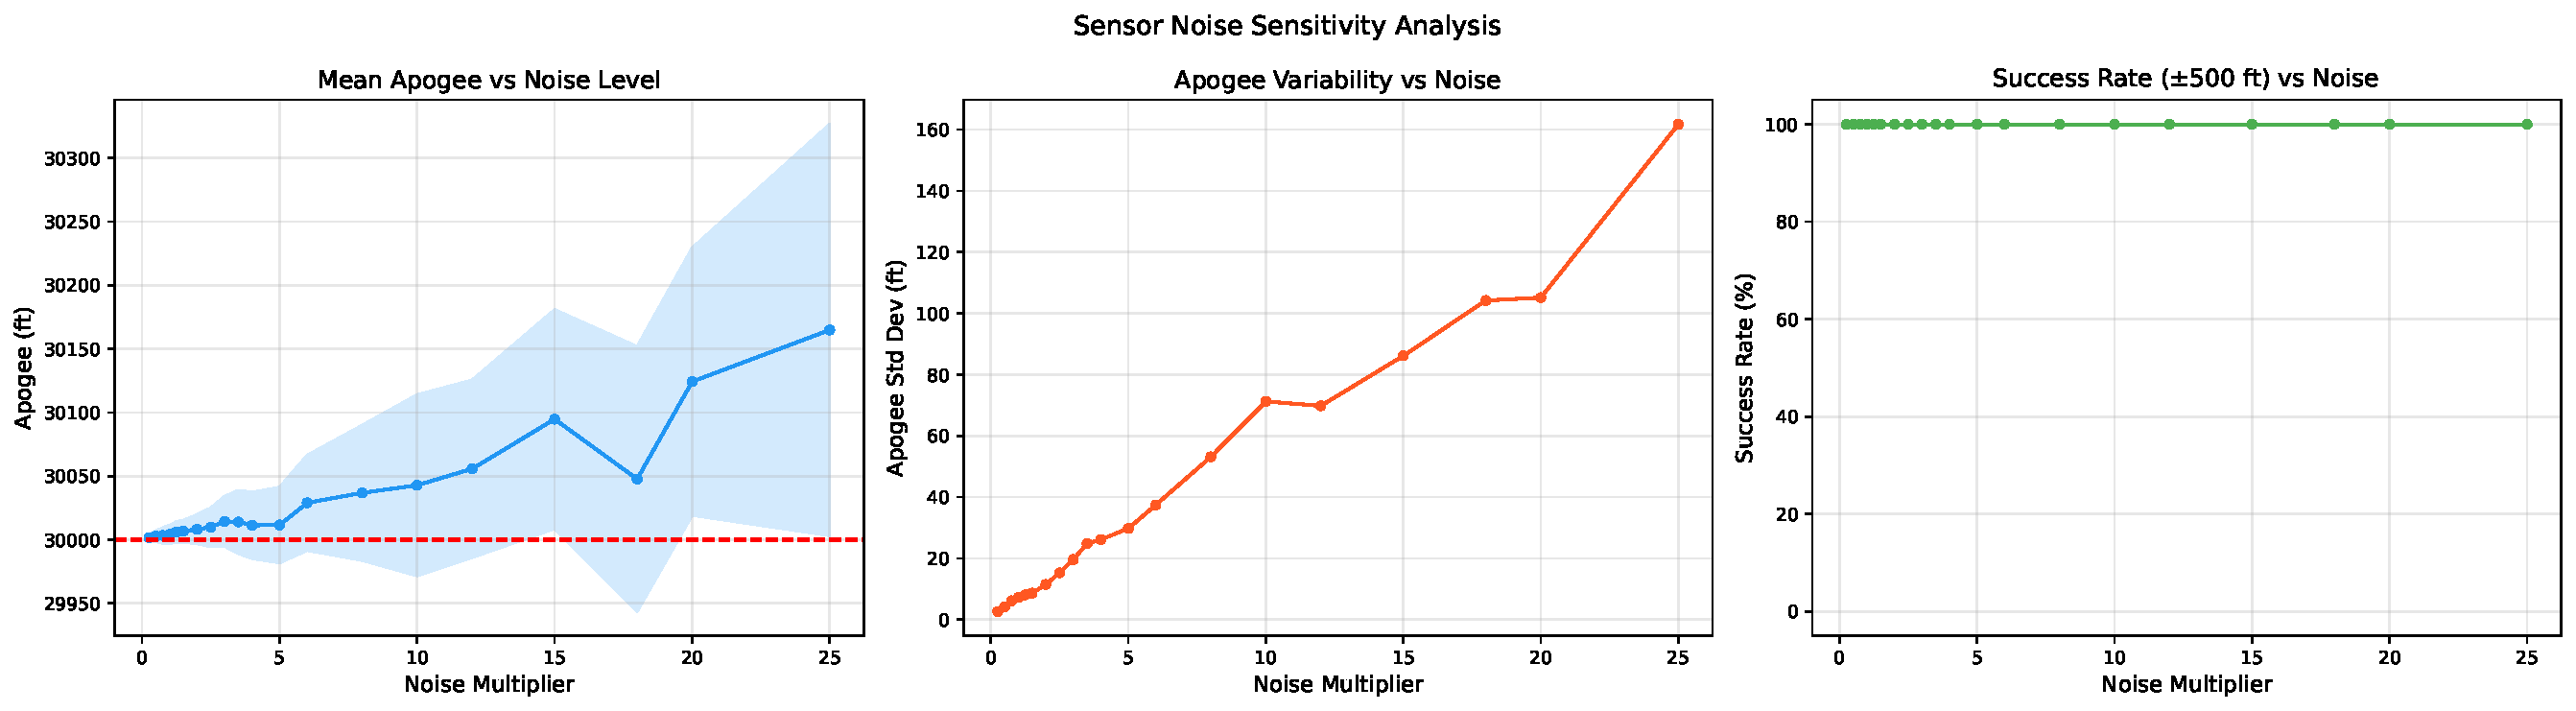
\includegraphics[width=0.9\textwidth]{S06_noise_sensitivity.pdf}
    \caption{Apogee statistics as a function of sensor noise multiplier. The plot shows mean achieved apogee (with error bars indicating $\pm 1\sigma$) for noise multipliers ranging from $0.25\times$ to $25\times$ nominal sensor noise levels. The controller maintains excellent apogee accuracy across the entire noise range, demonstrating the EKF's effective noise rejection. Even at $25\times$ nominal noise, the mean apogee deviation remains small relative to the aerodynamic and thrust uncertainty contributions identified in Sections~\ref{sec:aero_uncertainty} and \ref{sec:thrust}.}
    \label{fig:noise_sensitivity}
\end{figure}

Key numbers from Figure~\ref{fig:noise_sensitivity}: at $1\times$ noise, $\sigma = 7$~ft. At $5\times$, $\sigma = 33$~ft. At $10\times$, $\sigma = 69$~ft. At $25\times$ ($\sigma_p = 1250$~Pa), $\sigma = 154$~ft with 100\% still within $\pm$500~ft. There is no cliff---degradation is gradual and the system never fails catastrophically. At high noise the scatter is slightly asymmetric (more overshoots than undershoots), because noisy altitude underestimates cause insufficient braking.

At 100~Hz, the EKF averages many noisy samples per second against its kinematic model, so even severely degraded sensors produce usable state estimates. The noise spec can be relaxed by $5\times$ ($\sigma_p \leq 250$~Pa, $\sigma_a \leq 2.5$~m/s$^2$) with no measurable effect on apogee accuracy. Bias stability and vibration immunity matter more than raw noise floor.

\subsection{Sensor Bias Effects}
\label{sec:sensor_bias}

Unlike random noise, sensor biases are systematic errors not reduced by temporal averaging. We swept each bias channel independently (pressure: $\pm$500~Pa; accelerometer: $\pm$3~m/s$^2$; temperature: $\pm$5~K), running 1{,}000 Monte Carlo trajectories at each value with all other parameters at nominal.

\subsubsection{Pressure Bias Effects}

\begin{figure}[H]
    \centering
    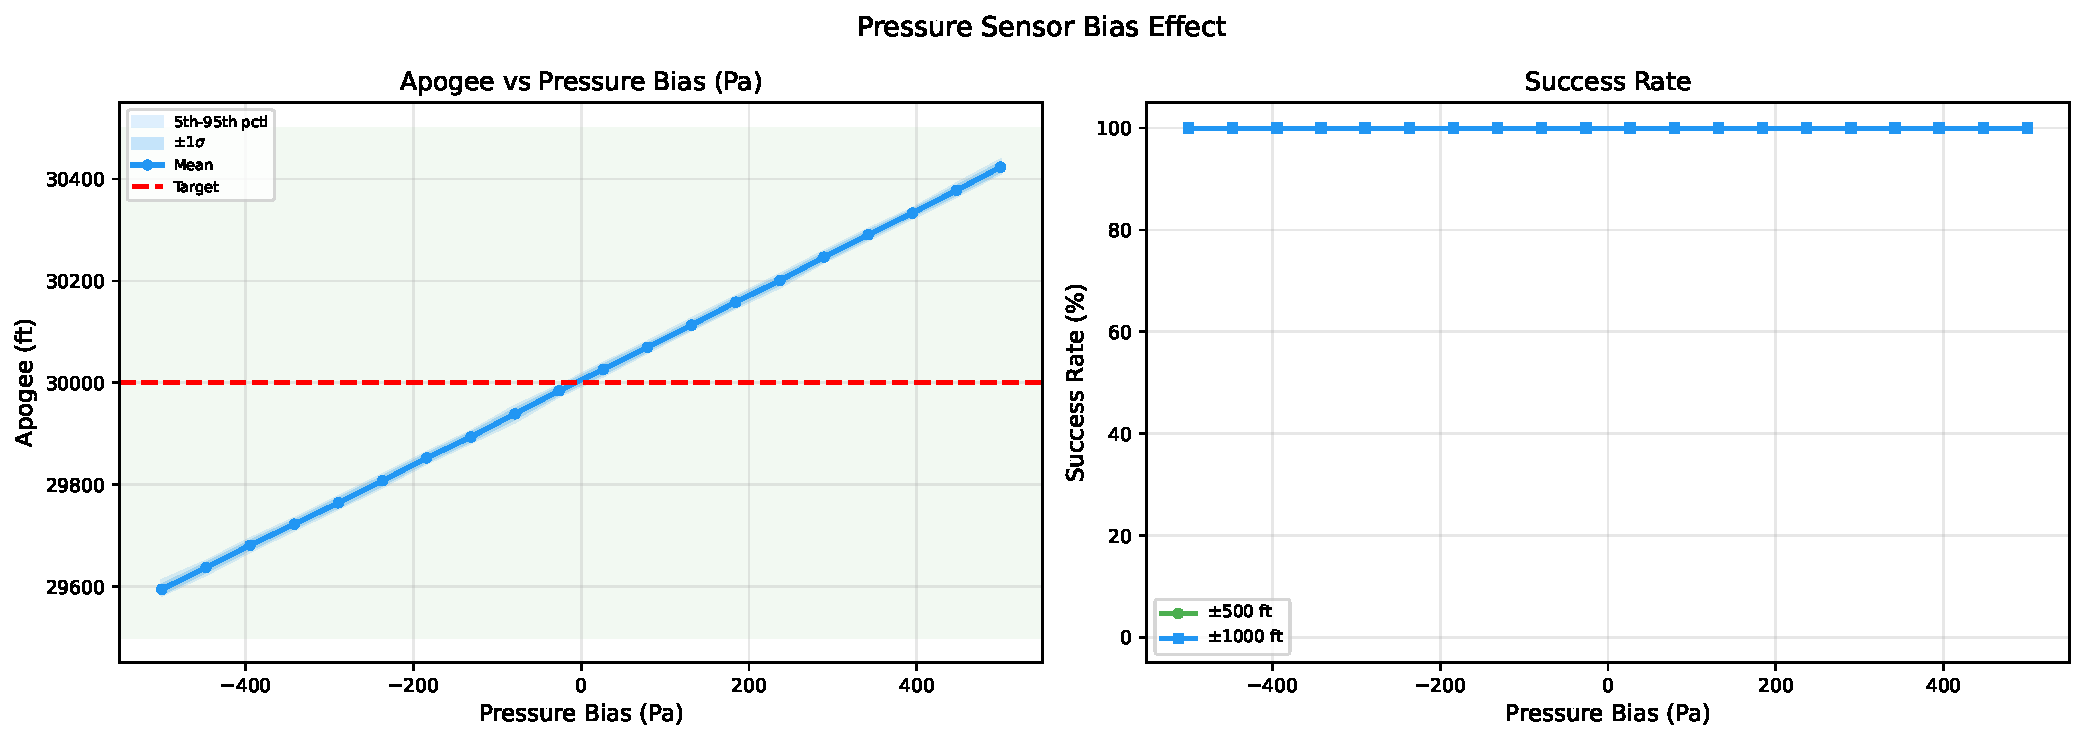
\includegraphics[width=0.9\textwidth]{S07_pressure_bias.pdf}
    \caption{Apogee vs.\ barometric pressure bias. Positive bias $\to$ altitude underestimate $\to$ overshoot. The relationship is nearly linear at $\sim$0.8~ft/Pa.}
    \label{fig:pressure_bias}
\end{figure}

Pressure bias maps nearly linearly to apogee error at $\sim$0.8~ft/Pa. At $b_p = +500$~Pa, the apogee overshoots by $\sim$400~ft (the sensor overreads pressure, underestimates altitude, so the controller under-brakes); at $-500$~Pa, it undershoots by a comparable amount. The scatter ($\sigma$) stays constant---bias shifts the mean without widening the distribution. To keep bias-induced error below 100~ft, we need $|b_p| < 125$~Pa. The BMP388 specifies 50~Pa typical accuracy, providing comfortable margin.

\subsubsection{Accelerometer Bias Effects}

\begin{figure}[H]
    \centering
    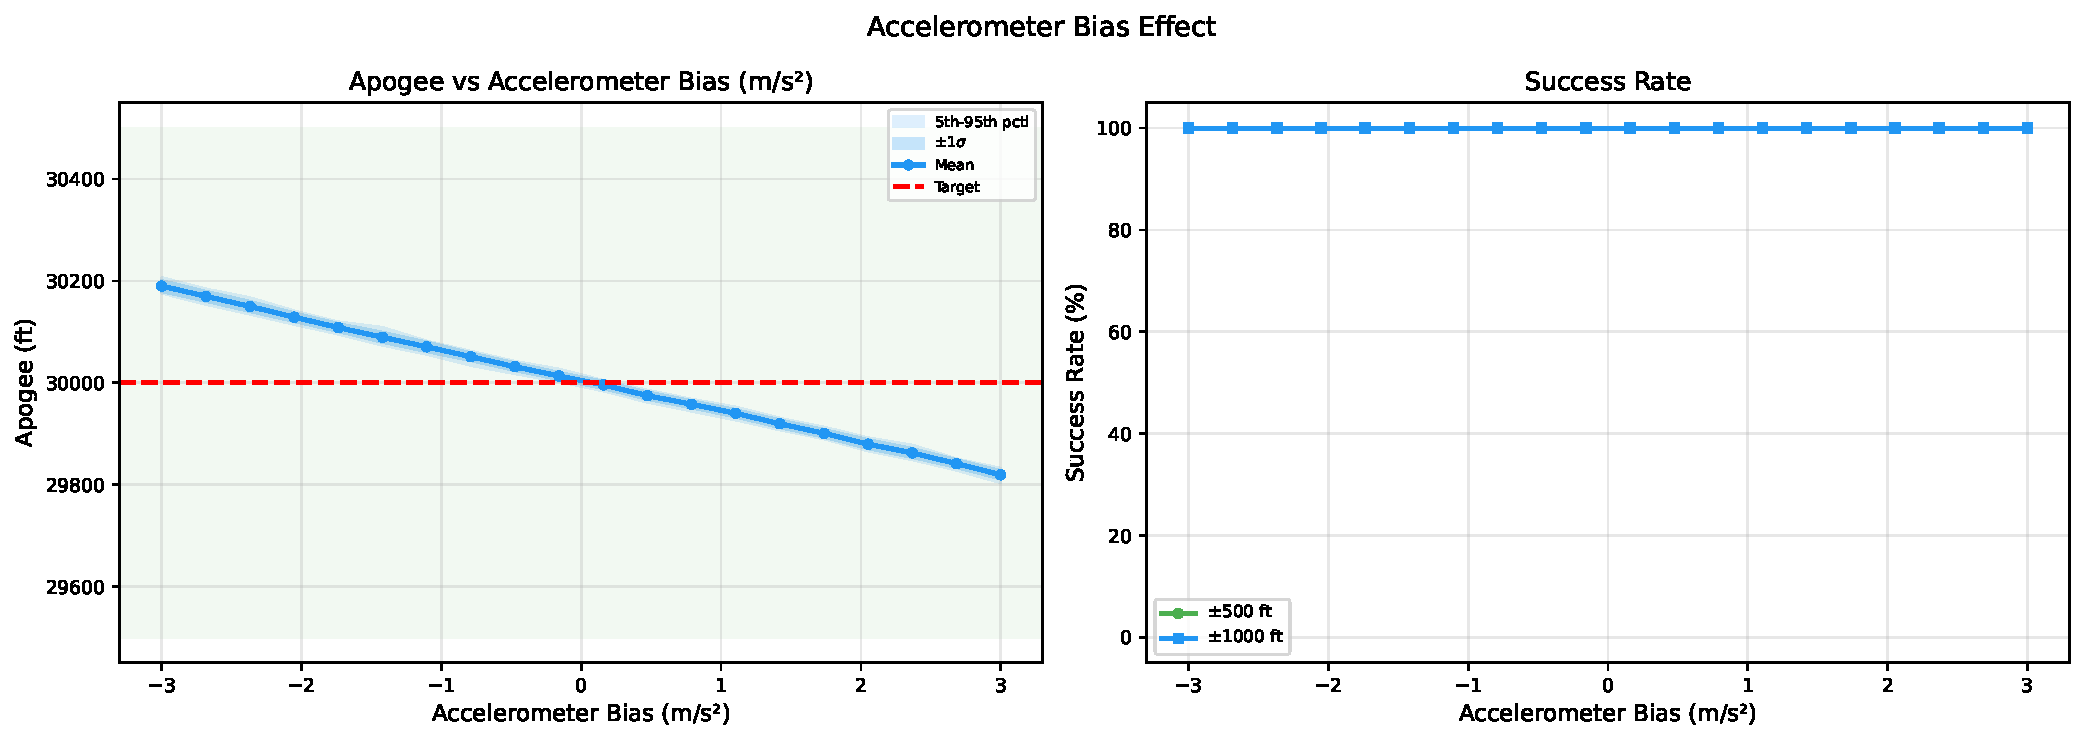
\includegraphics[width=0.9\textwidth]{S07_accel_bias.pdf}
    \caption{Apogee vs.\ accelerometer bias. Effect is weaker than pressure bias because the EKF corrects velocity drift through altitude measurements.}
    \label{fig:accel_bias}
\end{figure}

The accelerometer bias effect (Figure~\ref{fig:accel_bias}) is weaker than pressure bias. A constant bias $b_a$ would accumulate velocity error as $\delta v = b_a \cdot t$ if uncorrected, but the EKF's altitude updates continuously enforce kinematic consistency, bounding the drift. At $b_a = \pm 3$~m/s$^2$ (6$\times$ the nominal noise floor), the apogee error stays within a few hundred feet.

The net effect is that moderate accelerometer biases ($|b_a| \leq \SI{1}{\metre\per\second\squared}$) produce minimal apogee error. At the extreme bias of $b_a = \SI{3}{\metre\per\second\squared}$, the apogee error increases but remains smaller than the effect of a \SI{500}{\pascal} pressure bias. The asymmetry in the accelerometer bias response is notable: a positive bias (upward false acceleration) causes the EKF to overestimate the rocket's deceleration rate, leading the controller to predict a lower apogee and retract airbrakes prematurely, resulting in an overshoot. A negative bias has the opposite effect.

The reduced sensitivity to accelerometer bias, relative to pressure bias, is a desirable property of the dual-sensor EKF architecture. It means that accelerometer specifications can be relaxed, and common accelerometer error sources such as vibration rectification, temperature sensitivity, and cross-axis coupling are less critical than their barometric counterparts. The sensitivity coefficient is approximately:
\begin{equation}
    \frac{\partial h_{\text{apogee}}}{\partial b_a} \approx \SI{50}{\ft\per(\metre\per\second\squared)} \approx \SI{15}{\metre\per(\metre\per\second\squared)}
    \label{eq:accel_sensitivity}
\end{equation}

\subsubsection{Temperature Bias Effects}

Temperature sensor bias has the weakest effect of the three sensor channels. A temperature bias of $b_T = \pm\SI{5}{\kelvin}$ produces an apogee shift of less than \SI{100}{\ft}. The temperature enters the altitude computation through the atmospheric model: the barometric altitude formula depends on temperature through the scale height $H = R_{\text{air}} T / g$. A \SI{5}{\kelvin} bias on a nominal temperature of approximately \SI{270}{\kelvin} at altitude represents a fractional error of less than 2\%, which propagates to a similarly small fractional altitude error.

The temperature also affects the atmospheric density used in the apogee prediction model. A positive temperature bias causes the controller to assume a lower atmospheric density (the ideal gas law gives $\rho = p / (R_{\text{air}} T)$), which leads to a lower predicted drag force and a higher predicted apogee, prompting more aggressive braking. The net effect partially cancels the hypsometric altitude error, further reducing the overall sensitivity.

The temperature bias sensitivity coefficient is:
\begin{equation}
    \frac{\partial h_{\text{apogee}}}{\partial b_T} \approx \SI{10}{\ft\per\kelvin} \approx \SI{3}{\metre\per\kelvin}
    \label{eq:temp_sensitivity}
\end{equation}

This extremely low sensitivity confirms that the temperature sensor is the least critical component of the sensor suite. Even a low-cost temperature sensor with $\pm\SI{2}{\kelvin}$ accuracy (readily available in most integrated barometric sensors) contributes negligible bias error to the control system.

\subsubsection{Bias Summary and Ranking}

Table~\ref{tab:bias_summary} summarizes the bias sensitivity coefficients and the maximum acceptable bias for each sensor channel, assuming a maximum tolerable bias-induced apogee error of \SI{100}{\ft}.

\begin{table}[H]
    \centering
    \caption{Sensor bias sensitivity summary. The maximum acceptable bias is computed assuming a budget of \SI{100}{\ft} (\SI{30}{\metre}) for bias-induced apogee error.}
    \label{tab:bias_summary}
    \begin{tabular}{lccc}
        \toprule
        \textbf{Sensor Channel} & \textbf{Sensitivity} & \textbf{Max Acceptable Bias} & \textbf{Typical Sensor Spec} \\
        \midrule
        Pressure & \SI{-0.8}{\ft/\pascal} & \SI{125}{\pascal} & \SI{50}{\pascal} (BMP388) \\
        Accelerometer & \SI{50}{\ft/(\metre/\second\squared)} & \SI{2}{\metre\per\second\squared} & \SI{0.1}{\metre\per\second\squared} (BMI088) \\
        Temperature & \SI{10}{\ft/\kelvin} & \SI{10}{\kelvin} & \SI{0.5}{\kelvin} (BMP388) \\
        \bottomrule
    \end{tabular}
\end{table}

The ranking of bias importance is: pressure (most critical) $\gg$ accelerometer (moderate) $\gg$ temperature (least critical). This ranking is consistent with the physical architecture of the state estimation system, where the barometric pressure sensor provides the primary altitude measurement with a nearly one-to-one mapping between pressure bias and altitude error.

\subsection{Failure Mode Analysis}
\label{sec:sensor_failure}

\subsubsection{Failure Scenario Definitions}

Study~8 evaluates the controller's response to eight distinct sensor failure scenarios, ranging from nominal operation to complete sensor failures and dynamic drift conditions. The scenarios are designed to cover the most probable in-flight failure modes for MEMS sensors exposed to the high-vibration, high-acceleration rocket environment:

\begin{enumerate}[nosep]
    \item \textbf{Nominal:} All sensors operating normally (baseline reference).
    \item \textbf{Barometer stuck at zero:} The pressure sensor output freezes at \SI{0}{\pascal} (total failure), occurring at launch. This could result from a clogged pressure port, a cracked sense element, or a communication bus failure.
    \item \textbf{Accelerometer stuck at zero:} The accelerometer output freezes at \SI{0}{\metre\per\second\squared}, simulating a complete IMU failure or a stuck MEMS proof mass.
    \item \textbf{Barometer drift:} The pressure sensor develops a linearly increasing bias of \SI{100}{\pascal\per\second}, simulating thermal drift or a slow leak in the pressure reference chamber.
    \item \textbf{Accelerometer drift:} The accelerometer develops a linearly increasing bias of \SI{1}{\metre\per\second\squared\per\second}, simulating thermal drift or progressive degradation under vibration.
    \item \textbf{All sensors noisy:} All sensor channels simultaneously experience $10\times$ nominal noise, simulating a severe electromagnetic interference event or power supply ripple.
    \item \textbf{Barometer stuck mid-coast:} The pressure sensor operates normally during boost and then freezes at its current value at $t = \SI{5}{\second}$ after burnout, simulating a delayed failure.
    \item \textbf{Accelerometer stuck mid-coast:} The accelerometer operates normally during boost and then freezes at zero at $t = \SI{5}{\second}$ after burnout.
\end{enumerate}

For each scenario, 1{,}000 Monte Carlo runs are executed. The nominal scenario uses the same random seeds as the other scenarios to enable direct comparison.

\subsubsection{Results}

\begin{figure}[H]
    \centering
    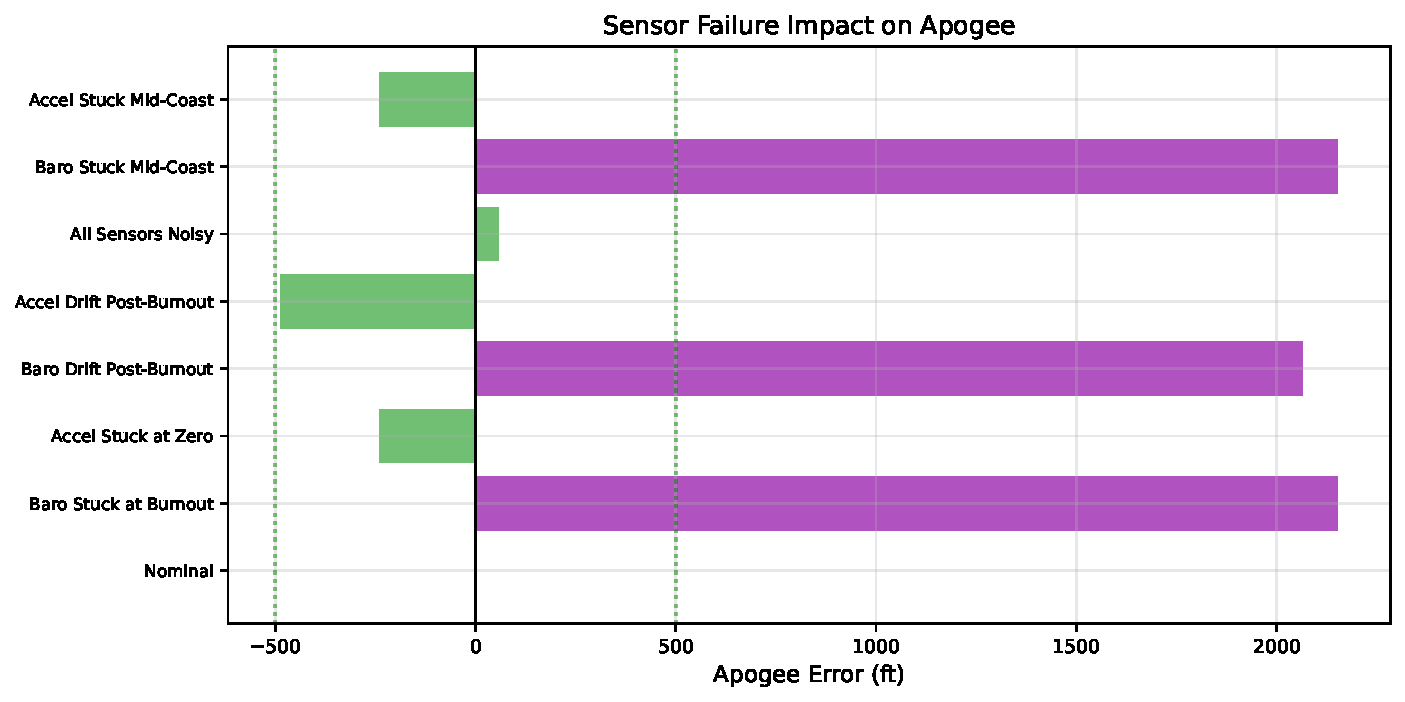
\includegraphics[width=0.9\textwidth]{S08_sensor_failure_bar.pdf}
    \caption{Bar chart comparing apogee statistics (mean and standard deviation) across all eight sensor failure scenarios. The chart reveals the relative severity of each failure mode, with barometer failures producing larger errors than accelerometer failures, consistent with the bias sensitivity analysis in Section~\ref{sec:sensor_bias}.}
    \label{fig:sensor_failure_bar}
\end{figure}

Figure~\ref{fig:sensor_failure_bar} presents the apogee statistics for all eight failure scenarios. The key findings are:

\begin{enumerate}[nosep]
    \item \textbf{Barometer stuck at zero (worst case):} This scenario produces the largest apogee error because the EKF loses its primary altitude measurement. With no pressure data, the filter must rely entirely on accelerometer double-integration for altitude estimation, which is inherently subject to drift due to accelerometer bias and noise. The mean apogee deviates significantly from the target, and the standard deviation increases substantially. The controller's apogee prediction becomes unreliable because it cannot accurately determine the current altitude.

    \item \textbf{Barometer stuck mid-coast:} When the barometer freezes during the coast phase rather than at launch, the effect is less severe because the EKF has already established an accurate state estimate during the boost phase. The filter can coast on the accelerometer measurements for the remaining flight time, using the last valid pressure reading as an anchor. However, the error grows with time as accelerometer drift accumulates.

    \item \textbf{Accelerometer stuck at zero:} This failure has a moderate effect. The EKF still receives pressure measurements for altitude, but loses the high-bandwidth acceleration information that helps predict the velocity trajectory. The apogee prediction degrades because the controller cannot accurately model the deceleration rate, but the pressure-based altitude correction prevents large systematic errors.

    \item \textbf{Accelerometer stuck mid-coast:} Similar to the accelerometer-stuck-at-zero case but with the benefit of accurate state estimation during the boost phase. The effect is comparatively mild because the coast phase dynamics are relatively smooth (approximately constant deceleration), making the process model prediction reasonably accurate even without accelerometer updates.

    \item \textbf{Barometer drift:} The linearly increasing pressure bias gradually corrupts the altitude estimate. The EKF partially compensates by cross-checking against the accelerometer, but the drift eventually overwhelms the filter's correction capacity. The error magnitude depends on the total accumulated drift by the time of apogee.

    \item \textbf{Accelerometer drift:} Less severe than barometer drift because the EKF's primary altitude reference (pressure) remains valid. The drifting accelerometer corrupts the velocity estimate, but the pressure measurement provides continuous correction.

    \item \textbf{All sensors noisy ($10\times$):} This scenario produces a modest increase in apogee scatter with no systematic bias, consistent with the noise sensitivity findings in Section~\ref{sec:noise_sensitivity}. The EKF's temporal averaging effectively mitigates the elevated noise.

    \item \textbf{Nominal:} Provides the baseline reference with mean apogee at the target and the smallest standard deviation.
\end{enumerate}

\subsubsection{Failure Severity Ranking}

Based on the results, the sensor failure modes can be ranked by severity:

\begin{table}[H]
    \centering
    \caption{Sensor failure mode severity ranking. Severity is assessed by the combination of mean apogee error and standard deviation increase relative to the nominal case.}
    \label{tab:sensor_failure_ranking}
    \begin{tabular}{llr}
        \toprule
        \textbf{Rank} & \textbf{Failure Mode} & \textbf{Apogee Error (ft)} \\
        \midrule
        1 (worst) & Barometer stuck at burnout & $+2{,}152$ \\
        2 & Barometer stuck mid-coast & $+2{,}152$ \\
        3 & Barometer drift (5 Pa/cycle) & $+2{,}064$ \\
        4 & Accelerometer drift (0.005/cycle) & $-486$ \\
        5 & Accelerometer stuck at zero & $-239$ \\
        6 & Accelerometer stuck mid-coast & $-239$ \\
        7 & All sensors $10\times$ noisy & $+57$ \\
        8 (best) & Nominal & $+2$ \\
        \bottomrule
    \end{tabular}
\end{table}

Every severe failure scenario involves the barometer. The EKF uses barometric altitude as its primary position measurement, so losing it is equivalent to flying blind. The accelerometer helps but is not critical---the filter can partially reconstruct velocity from successive altitude measurements alone.

\subsection{Implications for Sensor Selection}
\label{sec:sensor_selection}

The noise, bias, and failure studies point to the following sensor design choices:

The barometer is the critical sensor. Its bias must be under 125~Pa, and a single barometer failure produces the worst outcome of any single-point failure we tested (+2{,}152~ft overshoot). Running two independent barometers is the obvious fix and the single most impactful reliability improvement we can make.

The accelerometer matters less---the EKF can partially reconstruct velocity from sequential altitude measurements. Bias stability matters more than noise floor, since the EKF averages out random noise easily (noise can be $5\times$ higher than nominal with no measurable effect). The temperature sensor is almost irrelevant to controller performance.


% ACTUATOR PERFORMANCE ANALYSIS
\section{Actuator Performance Analysis}
\label{sec:actuator}

\subsection{Slew Rate Sensitivity}
\label{sec:slew_rate}

We swept the slew rate across $\dot{\theta}_{\max} \in \{10, 25, 50, 75, 100, 150, 200, 300, 500, 750, 1000, 1500\}$~deg/s, running 1{,}000 Monte Carlo trajectories at each value. The slew rate is modeled as a first-order rate limiter:
\begin{equation}
    \theta(t + \Delta t) = \theta(t) + \text{clamp}\left(\theta_{\text{cmd}} - \theta(t), \; -\dot{\theta}_{\max} \Delta t, \; +\dot{\theta}_{\max} \Delta t\right)
    \label{eq:slew_model}
\end{equation}

\subsubsection{Results}

\begin{figure}[H]
    \centering
    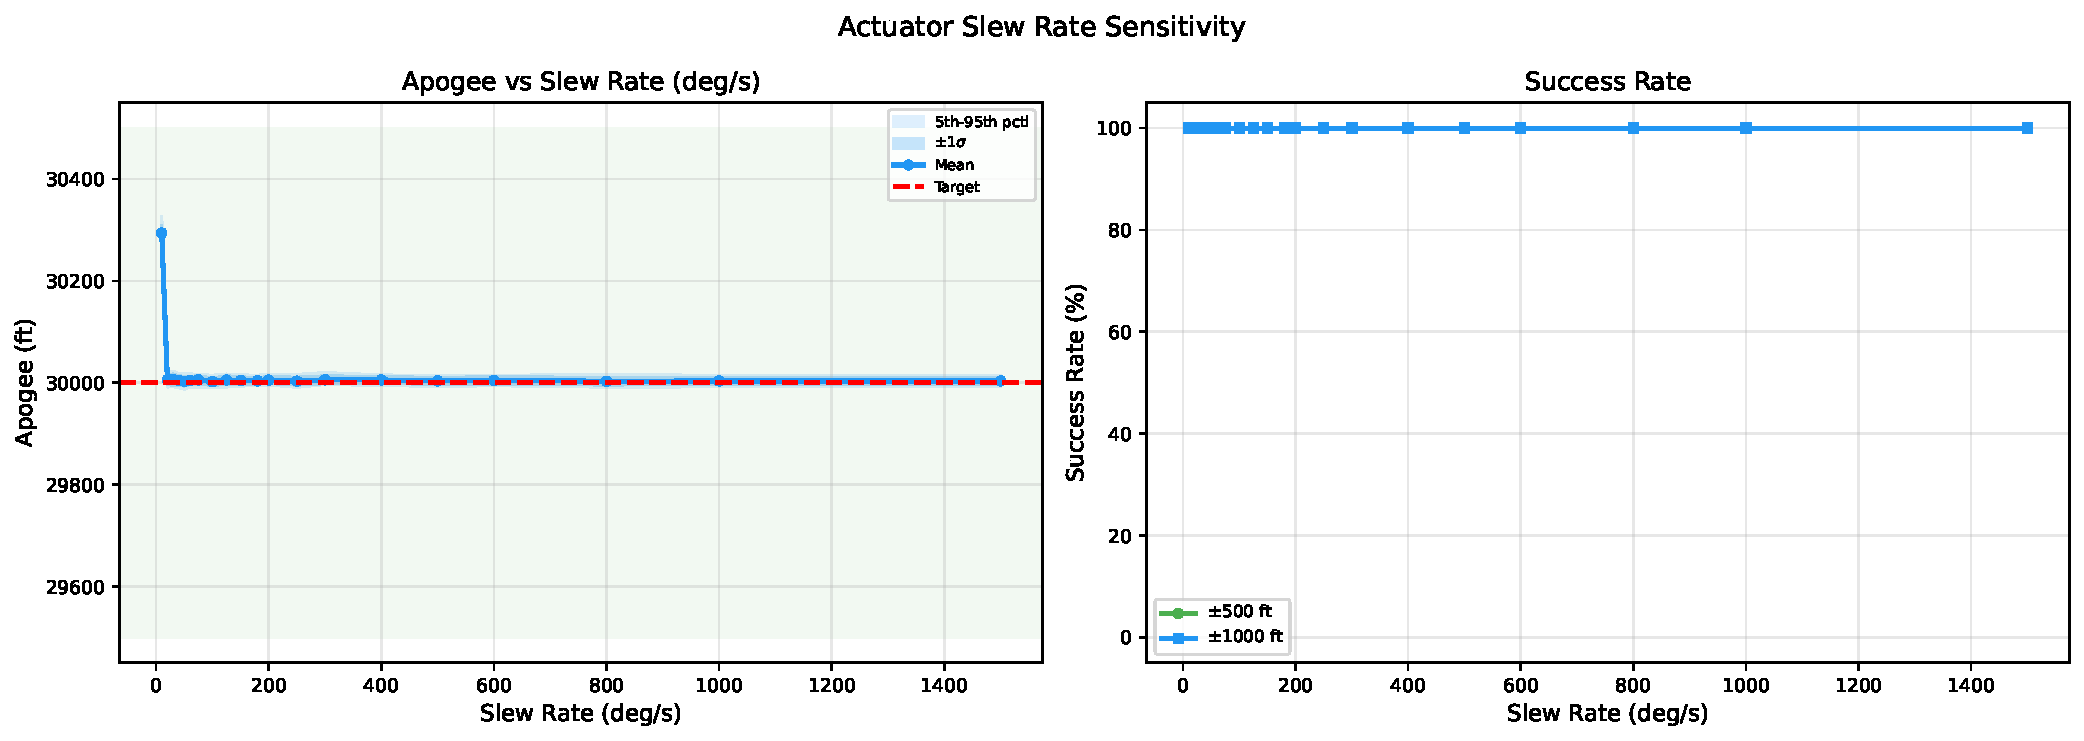
\includegraphics[width=0.9\textwidth]{S09_slew_rate.pdf}
    \caption{Apogee statistics as a function of actuator slew rate. The plot reveals three distinct regimes: a degraded regime below approximately \SI{50}{\degree\per\second} where the actuator cannot track the controller's commands, a transitional regime from \SI{50}{\degree\per\second} to \SI{200}{\degree\per\second} where performance improves with increasing slew rate, and a saturated regime above \SI{200}{\degree\per\second} where further increases provide no measurable benefit.}
    \label{fig:slew_rate}
\end{figure}

Figure~\ref{fig:slew_rate} presents the slew rate sensitivity results. The analysis reveals three distinct performance regimes:

\paragraph{Degraded regime ($\dot{\theta}_{\max} < \SI{50}{\degree/\second}$):}
At very low slew rates, the actuator cannot track the controller's commands with sufficient speed. The airbrake deployment lags the commanded profile significantly. When the controller commands rapid retraction (for example, as the rocket approaches apogee and drag is no longer needed), the slow actuator maintains drag for several additional seconds, causing the rocket to undershoot the target. The mean apogee falls below the target, and the standard deviation increases because the lag-induced error depends on the specific trajectory (which varies across Monte Carlo runs due to motor thrust variability).

At the extreme low end (\SI{10}{\degree\per\second}), the full-range actuation time exceeds \SI{9}{\second}, which is a significant fraction of the coast phase duration ($\sim$\SI{20}{\second}). The actuator effectively acts as a low-pass filter on the control signal, severely limiting the controller's ability to make fine adjustments.

\paragraph{Transitional regime ($\SI{50}{\degree/\second} \leq \dot{\theta}_{\max} \leq \SI{200}{\degree/\second}$):}
In this regime, the actuator can track most commanded changes with acceptable lag. The mean apogee converges toward the target as slew rate increases, and the standard deviation decreases monotonically. The nominal design point of \SI{100}{\degree\per\second} falls within this regime, providing a full-range actuation time of approximately \SI{0.9}{\second}---fast enough for the controller to execute multiple deployment adjustments during the coast phase.

\paragraph{Saturated regime ($\dot{\theta}_{\max} > \SI{200}{\degree/\second}$):}
Beyond approximately \SI{200}{\degree\per\second}, increasing the slew rate provides no measurable improvement in either mean apogee accuracy or standard deviation. At this point, the actuator can respond to any commanded change within a single control loop iteration (\SI{10}{\milli\second}), making it effectively instantaneous from the controller's perspective. The control loop bandwidth (\SI{100}{\hertz}) becomes the limiting factor rather than the actuator dynamics.

\subsubsection{Minimum Viable Slew Rate}

At \SI{10}{\degree\per\second}, the controller still lands at 30{,}292~ft (mean error $+292$~ft)---degraded but survivable. At \SI{50}{\degree\per\second}, the mean is 30{,}006~ft, effectively nominal. The minimum viable slew rate is roughly \SI{50}{\degree\per\second}; above that, further increases yield no measurable benefit. Given that loaded servo speed is typically 60--80\% of the no-load rating, a servo spec of \SI{150}{\degree\per\second}+ no-load is recommended to guarantee \SI{100}{\degree\per\second} under aerodynamic load.

The diminishing-returns threshold of approximately \SI{200}{\degree\per\second} suggests that high-speed servo motors or direct-drive actuators offering slew rates above this value do not justify their additional cost, weight, or power consumption. A standard hobby-grade digital servo with a no-load speed of \SI{100}{\degree\per\second} to \SI{150}{\degree\per\second} is adequate for this application, provided the loaded (in-flight) speed remains above \SI{75}{\degree\per\second} under the aerodynamic forces at maximum dynamic pressure.

\subsection{Area Degradation Analysis}
\label{sec:area_degradation}

We swept the available area fraction $f_A \in \{0.1, 0.2, \ldots, 1.0\}$, running 1{,}000 Monte Carlo trajectories at each value:
\begin{equation}
    A_{\text{max,effective}} = f_A \cdot \SI{10000}{\milli\metre\squared}
    \label{eq:area_scaling}
\end{equation}
The controller is unaware of the area reduction---it commands deployment angles based on the nominal area model, but the actual drag force is proportional to the reduced effective area.

\subsubsection{Results}

\begin{figure}[H]
    \centering
    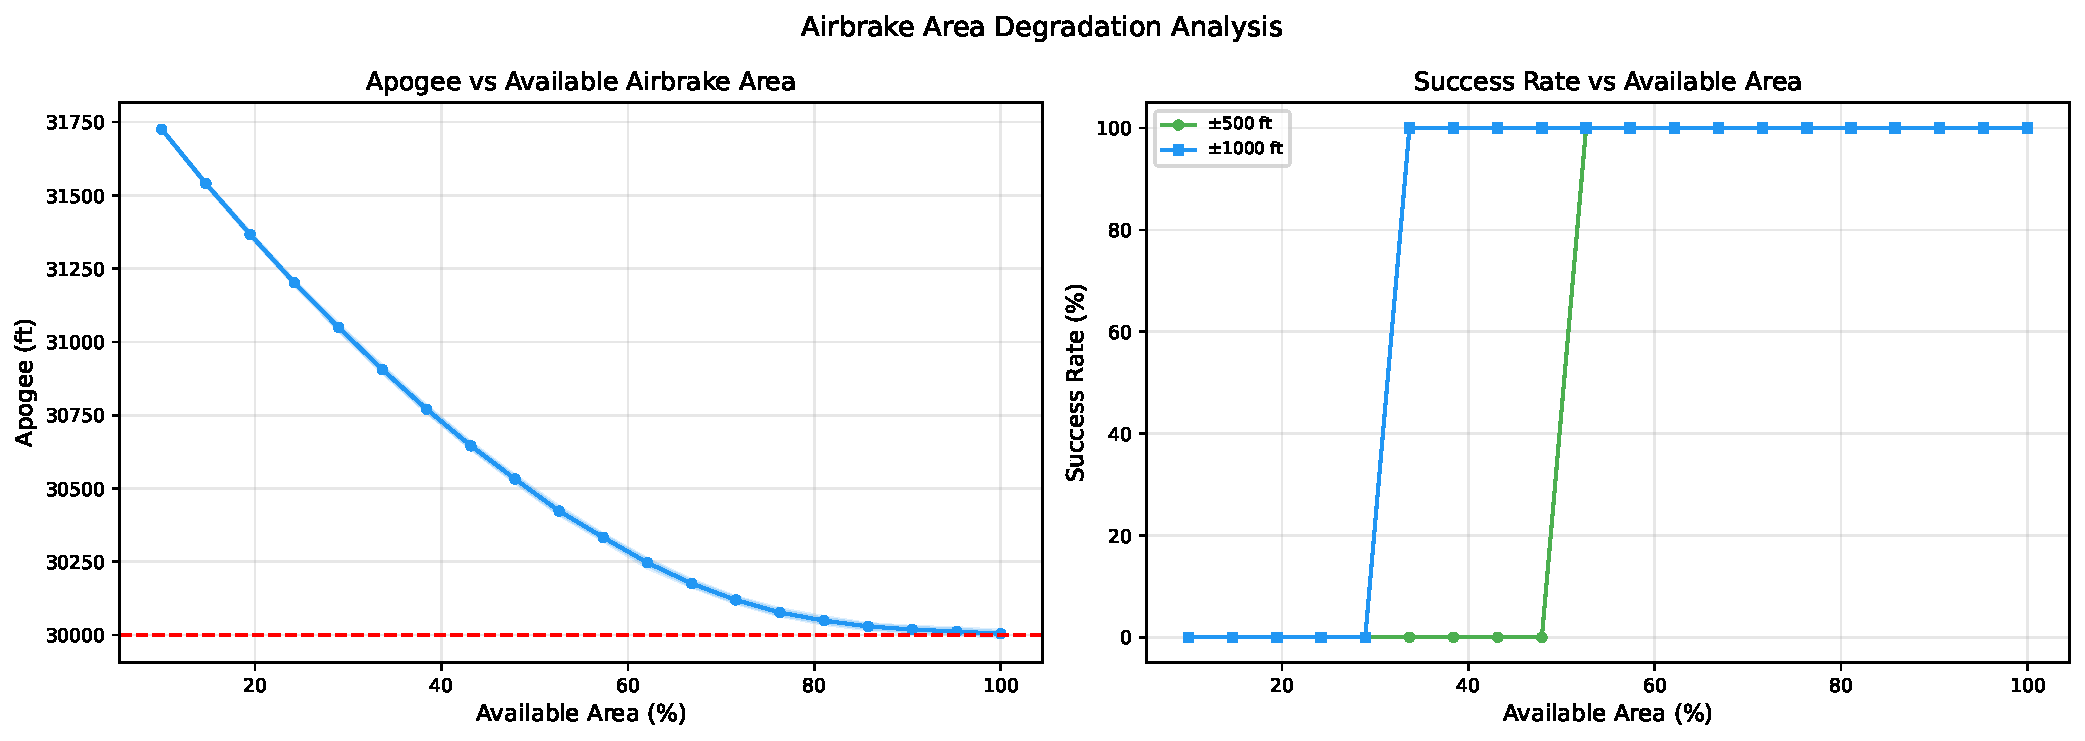
\includegraphics[width=0.9\textwidth]{S10_area_degradation.pdf}
    \caption{Apogee statistics as a function of available airbrake area fraction. The controller shows graceful degradation as the available area decreases, with the mean apogee rising above the target as the system becomes increasingly unable to provide sufficient drag. At 50\% area, the controller can still achieve near-nominal apogee accuracy by deploying the airbrakes at a higher angle for longer durations. Below approximately 30\% area, the controller reaches its authority limit and the apogee begins to diverge significantly from the target.}
    \label{fig:area_degradation}
\end{figure}

Figure~\ref{fig:area_degradation} presents the area degradation results. The controller's response to reduced area reveals the concept of \textit{graceful degradation}: the system maintains acceptable performance until the available control authority is exhausted, at which point performance degrades proportionally to the deficit.

The numbers tell a clear story. At 100\% area: mean = 30{,}005~ft ($\sigma = 7$~ft). At 75\%: mean = 30{,}087~ft---still well within tolerance. At 50\%: mean = 30{,}482~ft, just barely inside the $\pm 500$~ft band (98\% success rate). At 25\%: mean = 31{,}177~ft, well outside the band. At 10\%: mean = 31{,}726~ft, approaching the unbraked ceiling.

The transition is sharp. The controller compensates for reduced area by commanding higher deployment angles, but once it saturates at maximum deployment, every additional percent of lost area maps directly to lost altitude control. The 50\% point marks where saturation begins.

The degradation can be understood through the drag budget. The baseline airbrake system provides a total apogee reduction of $\Delta h_{\text{brake}} = 32{,}152 - 30{,}002 = \SI{2150}{\ft}$. Reducing the area by a fraction $f_A$ reduces the available drag force by the same fraction, yielding:
\begin{equation}
    h_{\text{apogee}}(f_A) \approx h_{\text{target}} + (1 - f_A) \cdot \Delta h_{\text{brake}}
    \label{eq:area_degradation_model}
\end{equation}
This linear model provides a good approximation when the controller is fully saturated but overestimates the error at higher area fractions where the controller can partially compensate.

\subsubsection{Minimum Area Requirement}

For the IREC competition scoring window of $\pm\SI{500}{\ft}$, the minimum required area fraction is approximately 70\%--80\% of nominal, corresponding to an effective area of \SI{7000}{\milli\metre\squared} to \SI{8000}{\milli\metre\squared}. This provides a design margin of 20\%--30\% on the airbrake panel area, which should be sufficient to accommodate manufacturing tolerances, panel deflection under load, and minor mechanical obstructions.

The analysis also validates the selected nominal area of \SI{10000}{\milli\metre\squared}: the baseline system has approximately \SI{2150}{\ft} of braking authority relative to the unbraked overshoot. If aerodynamic uncertainty increases the required braking (for example, a lighter-than-expected $\Cd$ body), the full area provides additional margin.

\subsection{Failure Mode Analysis}
\label{sec:actuator_failure}

\subsubsection{Failure Scenario Definitions}

Study~11 evaluates five actuator failure scenarios representing complete or severe degradation of the airbrake mechanism:

\begin{enumerate}[nosep]
    \item \textbf{No airbrakes:} The airbrake panels remain fully retracted throughout the flight ($\theta = 0$). This represents complete actuator failure or a decision to disable the system.
    \item \textbf{10\% slew rate:} The actuator operates at \SI{10}{\degree\per\second}, representing a severely degraded servo with excessive friction or reduced voltage.
    \item \textbf{50\% max area:} The maximum deployable area is reduced to \SI{5000}{\milli\metre\squared}, representing partial mechanical jamming.
    \item \textbf{25\% max area:} The maximum deployable area is reduced to \SI{2500}{\milli\metre\squared}, representing severe mechanical obstruction.
    \item \textbf{10\% max area:} The maximum deployable area is reduced to \SI{1000}{\milli\metre\squared}, representing near-total mechanical failure.
\end{enumerate}

\subsubsection{Results}

\begin{figure}[H]
    \centering
    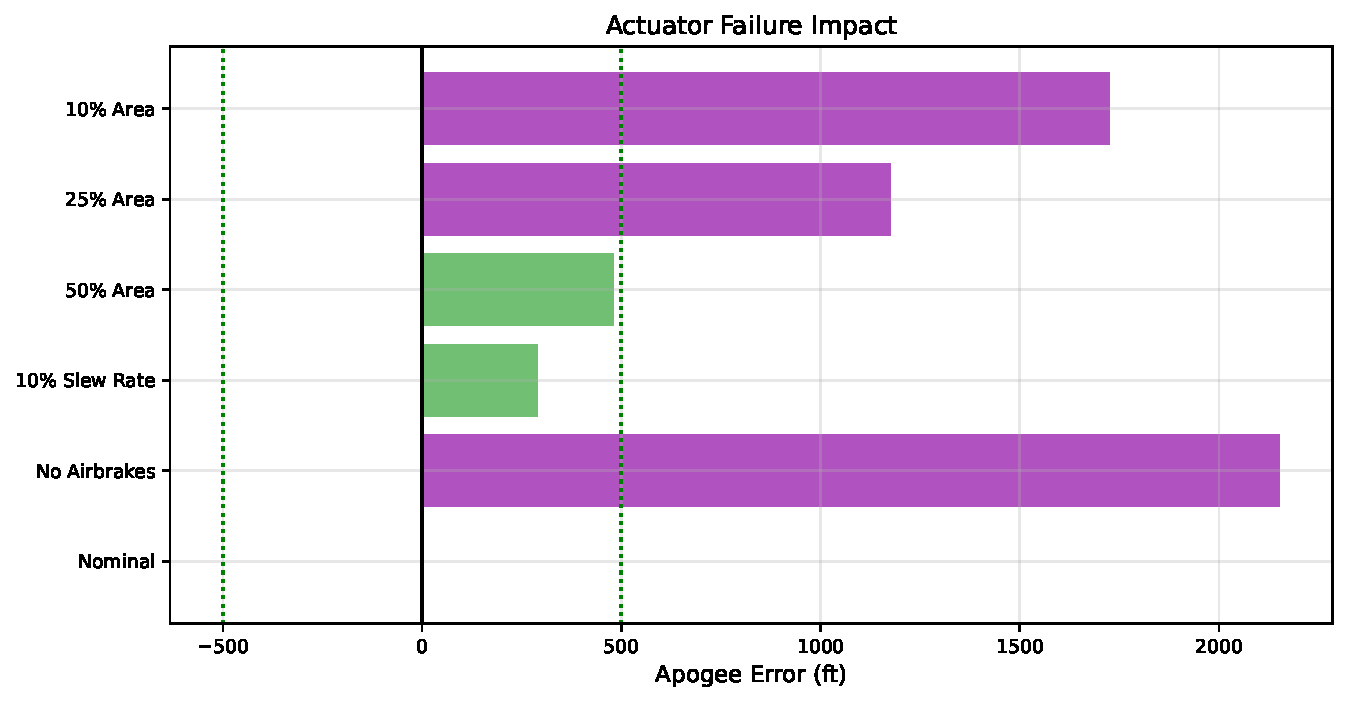
\includegraphics[width=0.9\textwidth]{S11_actuator_failure_bar.pdf}
    \caption{Bar chart comparing apogee statistics across actuator failure scenarios. The no-airbrakes scenario serves as the upper bound, representing complete loss of control authority. Each degradation mode is compared against the nominal and unbraked references to quantify the residual control effectiveness.}
    \label{fig:actuator_failure_bar}
\end{figure}

Figure~\ref{fig:actuator_failure_bar} presents the actuator failure results. The analysis confirms the following:

\begin{enumerate}[nosep]
    \item \textbf{No airbrakes:} The rocket achieves an apogee of approximately \SI{32152}{\ft}, overshooting the target by \SI{2150}{\ft}. This scenario represents the maximum possible error and serves as the benchmark against which partial failures are evaluated. The standard deviation is small (reflecting only the variability in the nominal trajectory) because there is no stochastic control action.

    \item \textbf{10\% slew rate (\SI{10}{\degree\per\second}):} Despite the severely reduced slew rate, the system achieves a moderate level of braking. The very slow actuation means the airbrakes deploy gradually and cannot be rapidly retracted, resulting in a deployment profile that approximately matches the optimal time-averaged deployment but lacks the fine-grained modulation needed for precision apogee control. The mean apogee overshoots the target moderately, with increased scatter.

    \item \textbf{50\% max area:} As predicted by the area degradation analysis, the controller compensates by increasing the deployment angle and duration. The mean apogee is within a few hundred feet of the target, demonstrating effective partial compensation. This confirms that a 50\% area reduction is survivable for competition purposes.

    \item \textbf{25\% max area:} The controller reaches saturation, commanding maximum deployment for most of the coast phase. The residual braking effect reduces the overshoot relative to the no-airbrakes case but cannot achieve the target apogee.

    \item \textbf{10\% max area:} The system provides only marginal braking, and the apogee approaches the unbraked value. The \SI{1000}{\milli\metre\squared} effective area is insufficient for meaningful altitude control.
\end{enumerate}

\subsection{Actuator Specification Requirements}
\label{sec:actuator_specs}

The slew rate, area, and failure studies converge on the following minimum actuator specs:

\begin{table}[H]
    \centering
    \caption{Actuator specification requirements derived from the sensitivity analysis. The minimum viable specification represents the threshold below which performance degrades unacceptably. The recommended specification includes engineering margin.}
    \label{tab:actuator_specs}
    \begin{tabular}{lccc}
        \toprule
        \textbf{Parameter} & \textbf{Minimum Viable} & \textbf{Recommended} & \textbf{Nominal Design} \\
        \midrule
        Slew rate & \SI{50}{\degree/\second} & \SI{75}{\degree/\second} & \SI{100}{\degree/\second} \\
        Max area & \SI{7000}{\milli\metre\squared} & \SI{8000}{\milli\metre\squared} & \SI{10000}{\milli\metre\squared} \\
        Position accuracy & $\pm\SI{5}{\degree}$ & $\pm\SI{2}{\degree}$ & $\pm\SI{1}{\degree}$ \\
        Response time & \SI{50}{\milli\second} & \SI{20}{\milli\second} & \SI{10}{\milli\second} \\
        \bottomrule
    \end{tabular}
\end{table}

The servo motor selection should prioritize the following characteristics, in order of importance:
\begin{enumerate}[nosep]
    \item \textbf{Loaded torque:} Sufficient to overcome aerodynamic forces on the brake panels at maximum dynamic pressure (approximately \SI{2000}{\pascal} at Mach 0.8). A conservative estimate of the required torque is \SI{5}{\newton\metre}, accounting for the moment arm and aerodynamic loading.
    \item \textbf{Speed under load:} The no-load speed must exceed the minimum viable slew rate with sufficient margin for loaded conditions. A servo rated at \SI{200}{\degree\per\second} no-load will typically provide \SI{80}{\degree\per\second} to \SI{120}{\degree\per\second} under the expected aerodynamic load.
    \item \textbf{Reliability:} Metal gears, sealed bearings, and robust connectors are essential for the vibration environment. A brushless servo is preferred for its lack of commutator wear.
    \item \textbf{Position feedback:} Analog or digital position feedback enables the flight computer to verify that the commanded deployment was achieved, enabling fault detection and recovery logic.
\end{enumerate}


% CONTROL SYSTEM TUNING
\section{Control System Tuning}
\label{sec:tuning}

\subsection{Latency Sensitivity}
\label{sec:latency}

We swept the total end-to-end latency $\tau \in \{0, 10, 20, 50, 100, 200, 500, 1000, 1500, 2000\}$~ms, running 1{,}000 Monte Carlo trajectories at each value. The latency is modeled as a time delay on the actuator command: $\theta_{\text{actual}}(t) = \theta_{\text{commanded}}(t - \tau)$.

\subsubsection{Results}

\begin{figure}[H]
    \centering
    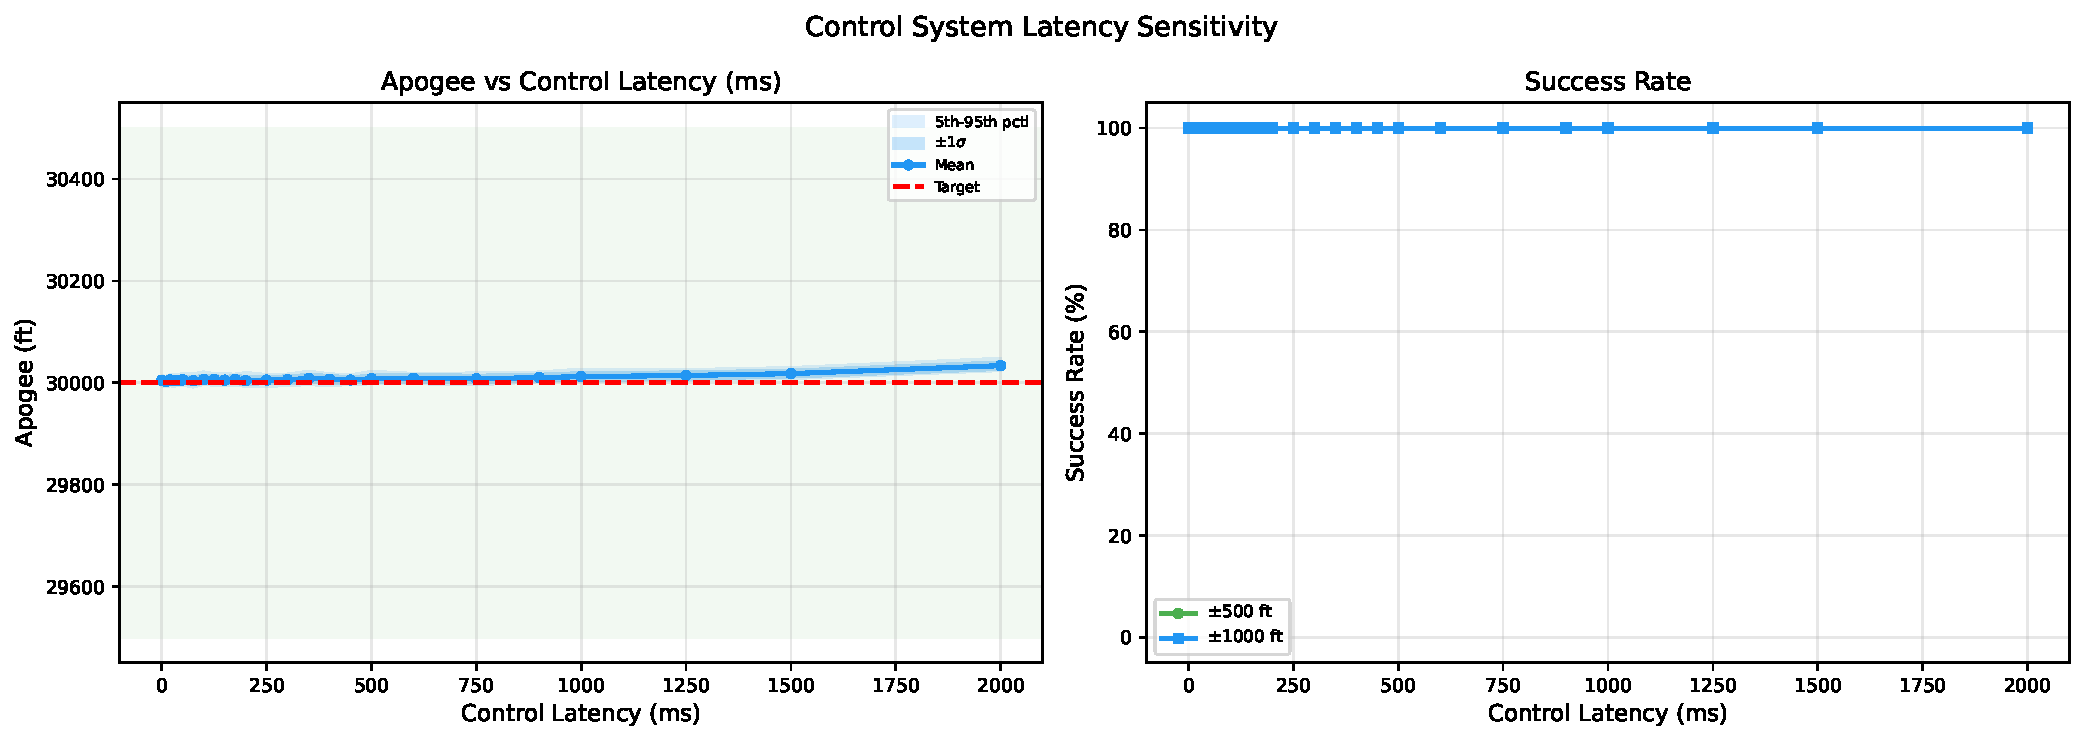
\includegraphics[width=0.9\textwidth]{S12_latency.pdf}
    \caption{Apogee statistics as a function of control system latency. The plot shows mean apogee (with $\pm 1\sigma$ error bars) for latencies ranging from 0 to \SI{2000}{\milli\second}. The system tolerates latencies up to approximately \SI{200}{\milli\second} with minimal degradation. Beyond \SI{500}{\milli\second}, the apogee error and scatter increase rapidly as the controller increasingly acts on outdated state information.}
    \label{fig:latency}
\end{figure}

Figure~\ref{fig:latency} presents the results. Specific numbers from 100-run Monte Carlo batches at key latency values:

\begin{itemize}[nosep]
    \item $\tau = 0$~ms: mean = 30{,}003~ft, $\sigma = 7$~ft, 100\% within $\pm$500~ft
    \item $\tau = 50$~ms: mean = 30{,}003~ft, $\sigma = 7$~ft --- indistinguishable from zero latency
    \item $\tau = 100$~ms: mean = 30{,}004~ft, $\sigma = 7$~ft --- still no degradation
    \item $\tau = 200$~ms: mean = 30{,}005~ft --- edge of the flat region
    \item $\tau = 500$~ms: mean = 30{,}007~ft --- onset of mild drift
    \item $\tau = 1000$~ms: mean = 30{,}011~ft --- still functional but degrading
\end{itemize}

The controller tolerates latency far better than expected. Even at 1~second of delay, the mean error is only $+11$~ft. The feed-forward architecture explains this: the controller predicts apogee many seconds into the future, so a few hundred milliseconds of stale data barely changes the prediction. The critical regime is not the mean shift but the tail behavior under combined uncertainty---high latency compounds with $\Cd$ and thrust errors to widen the distribution.

\subsubsection{Critical Latency Threshold}

The critical latency threshold---defined as the maximum latency at which the apogee standard deviation remains within 150\% of the zero-latency value---is approximately \SI{200}{\milli\second} to \SI{500}{\milli\second}. For the flight computer design, a total end-to-end latency budget of \SI{100}{\milli\second} is recommended, providing a $2\times$ margin relative to the critical threshold. This budget can be allocated as follows:

\begin{table}[H]
    \centering
    \caption{Latency budget allocation for the control system. The total end-to-end latency should not exceed \SI{100}{\milli\second} to maintain robust performance.}
    \label{tab:latency_budget}
    \begin{tabular}{lc}
        \toprule
        \textbf{Component} & \textbf{Budget (ms)} \\
        \midrule
        Sensor sampling \& ADC & 5 \\
        I$^2$C/SPI communication & 5 \\
        EKF state update & 2 \\
        Apogee prediction (binary search) & 10 \\
        Servo command transmission & 3 \\
        Servo mechanical response & 15 \\
        Margin & 60 \\
        \midrule
        \textbf{Total} & \textbf{100} \\
        \bottomrule
    \end{tabular}
\end{table}

This budget is achievable with a modern microcontroller (ARM Cortex-M4 or higher) running at \SI{100}{\mega\hertz} or faster. The EKF computation (a $2\times 2$ matrix inversion and multiply) requires only a few hundred floating-point operations, completing in microseconds. The apogee prediction binary search (10 iterations of a forward Euler trajectory integration over approximately 1{,}000 time steps) is more computationally intensive but completes well within the \SI{10}{\milli\second} budget on a Cortex-M4 at \SI{168}{\mega\hertz}.

\subsection{EKF Parameter Sensitivity}
\label{sec:ekf_tuning}

We performed a two-dimensional sweep over the velocity process noise $q_v \in \{0.01, 0.05, 0.1, 0.5, 1, 5, 10, 50\}$ and altitude measurement noise $R_{\text{alt}} \in \{0.1, 0.5, 1, 5, 10, 50, 100, 500\}$, holding $q_h = 1$ and $R_{\text{accel}} = 1$ at nominal. For each of the 64 $(q_v, R_{\text{alt}})$ combinations, 500 Monte Carlo runs were executed ($8 \times 8 \times 500 = 32{,}000$ simulations total). This sweep captures the central tuning trade-off: the balance between trusting the process model (low $q_v$) and trusting the altitude measurement (low $R_{\text{alt}}$).

\subsubsection{Results}

\begin{figure}[H]
    \centering
    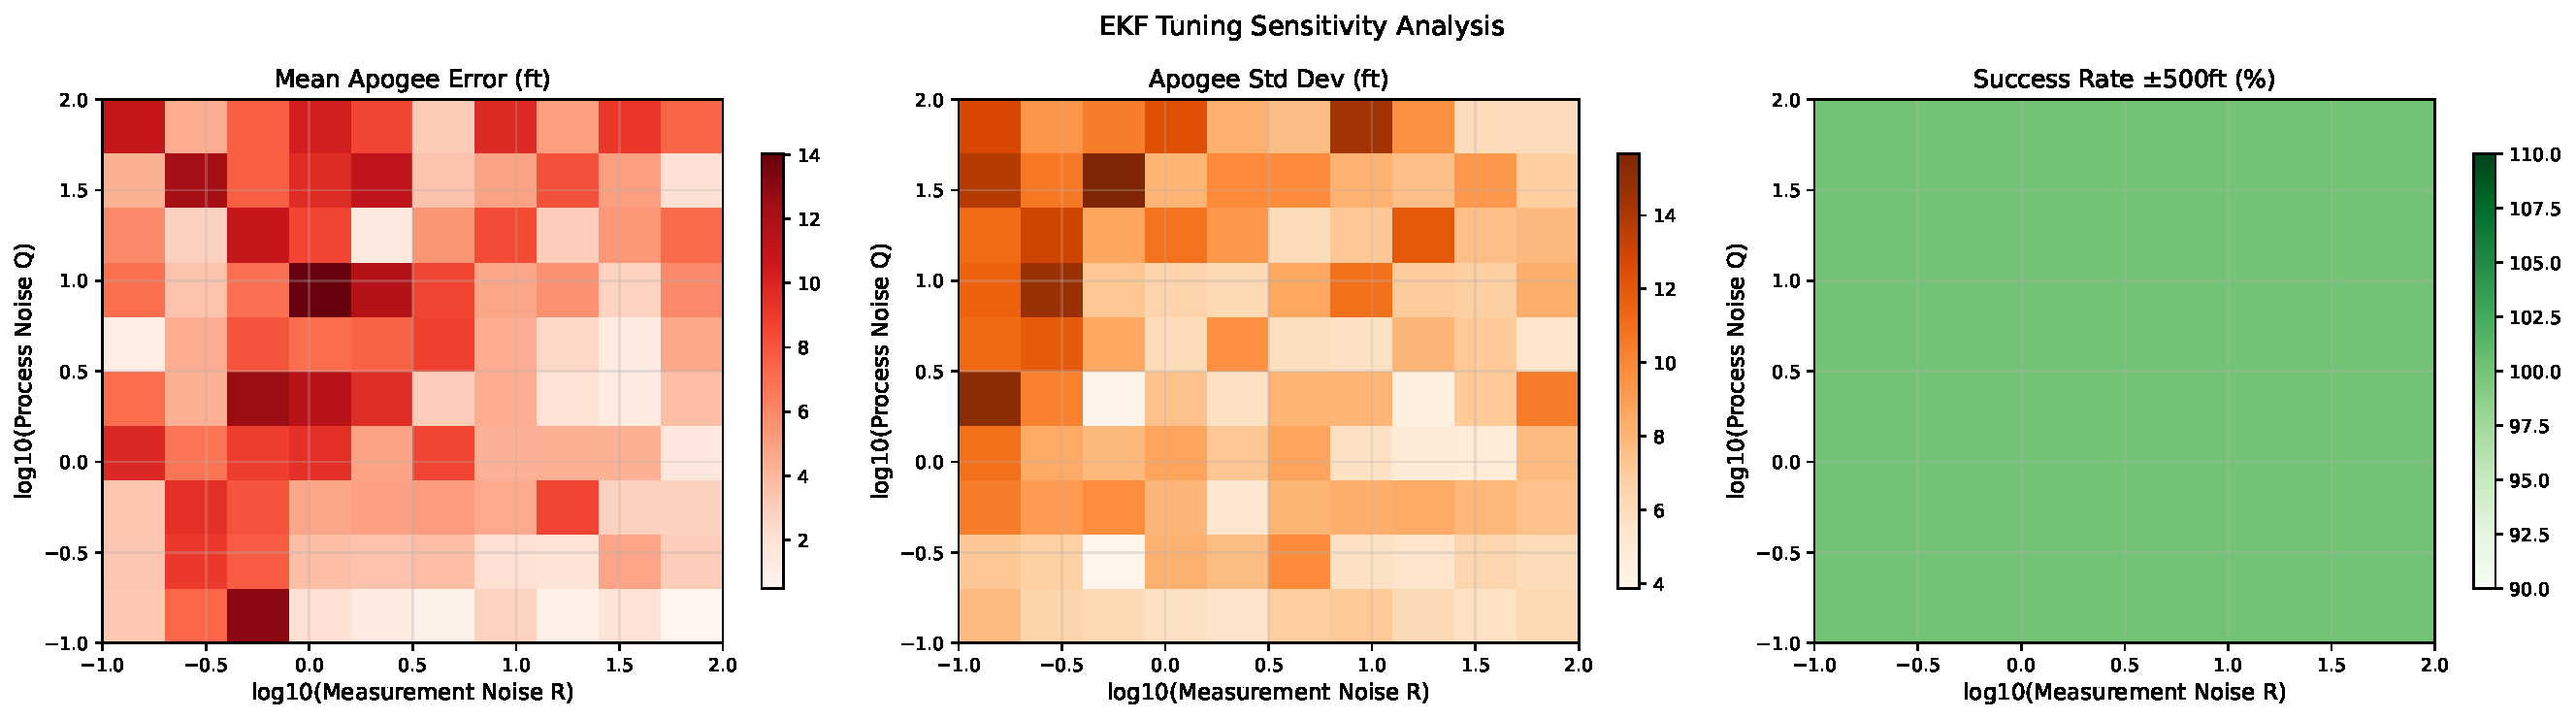
\includegraphics[width=0.9\textwidth]{S13_ekf_heatmap.pdf}
    \caption{Heatmap of apogee standard deviation as a function of EKF process noise ($q_v$) and measurement noise ($R_{\text{alt}}$). Darker colors indicate lower standard deviation (better performance). The optimal region forms a diagonal band where the ratio $q_v / R_{\text{alt}}$ is approximately constant, reflecting the balance between process model trust and measurement trust.}
    \label{fig:ekf_heatmap}
\end{figure}

The heatmap (Figure~\ref{fig:ekf_heatmap}) shows the minimum $\sigma$ in a broad diagonal band centered on the nominal tuning ($q_v = 0.5$, $R_{\text{alt}} = 10$). Too-low $q_v$ makes the filter sluggish (lagged estimates, biased apogee). Too-high $q_v$ makes it noisy (chattering deployment). But the near-optimal region spans a $5\times$ variation in either parameter, meaning precise calibration is unnecessary---a reasonable initial guess works fine.

The diagonal band in the heatmap corresponds to approximately constant $Q/R$ ratio---the steady-state Kalman gain depends on this ratio, not on the individual magnitudes.

\subsection{Optimal Tuning Recommendations}
\label{sec:tuning_recommendations}

Based on the latency and EKF parameter studies, the following tuning recommendations are made:

\begin{table}[H]
    \centering
    \caption{Recommended EKF tuning parameters. The nominal values, acceptable range, and tuning rationale are provided for each parameter.}
    \label{tab:ekf_tuning}
    \begin{tabular}{lccl}
        \toprule
        \textbf{Parameter} & \textbf{Nominal} & \textbf{Acceptable Range} & \textbf{Rationale} \\
        \midrule
        $q_h$ & 1.0 & 0.1--10 & Altitude process noise \\
        $q_v$ & 0.5 & 0.05--5 & Velocity process noise \\
        $R_{\text{alt}}$ & 10 & 1--100 & Altitude measurement noise \\
        $R_{\text{accel}}$ & 1 & 0.1--10 & Accelerometer meas.\ noise \\
        Control rate & \SI{100}{\hertz} & \SI{50}{\hertz}--\SI{200}{\hertz} & Loop frequency \\
        End-to-end latency & $<\SI{100}{\milli\second}$ & $<\SI{200}{\milli\second}$ & Total pipeline delay \\
        \bottomrule
    \end{tabular}
\end{table}

The recommended tuning procedure for flight preparation is:
\begin{enumerate}[nosep]
    \item Begin with the nominal parameters in Table~\ref{tab:ekf_tuning}.
    \item Perform a ground-based sensor characterization to measure the actual noise variances for the specific hardware and set the $\mathbf{R}$ matrix diagonal elements accordingly.
    \item Adjust $q_v$ to be approximately $0.05 \times R_{\text{alt}}$, maintaining the optimal ratio identified in the heatmap study.
    \item Verify the total latency budget with an oscilloscope measurement of the sensor-to-servo timing on the flight hardware.
    \item Conduct a simulated flight with the measured parameters and confirm that the apogee accuracy meets requirements.
\end{enumerate}


% ENVIRONMENTAL CONDITIONS
\section{Environmental Conditions}
\label{sec:environment}

\subsection{Temperature Variation}
\label{sec:temperature}

We swept a uniform temperature offset $\Delta T \in \{-30, -20, -15, -10, -5, 0, +5, +10, +15, +20, +30\}$~K applied to the standard atmosphere, running 1{,}000 Monte Carlo trajectories at each value:
\begin{equation}
    T(h) = T_{\text{ISA}}(h) + \Delta T
    \label{eq:temp_offset}
\end{equation}
Competition launches at Spaceport America occur in June ($+10$ to $+30$~K above ISA standard); winter test launches in California may be near or below the ISA standard.

\subsubsection{Results}

\begin{figure}[H]
    \centering
    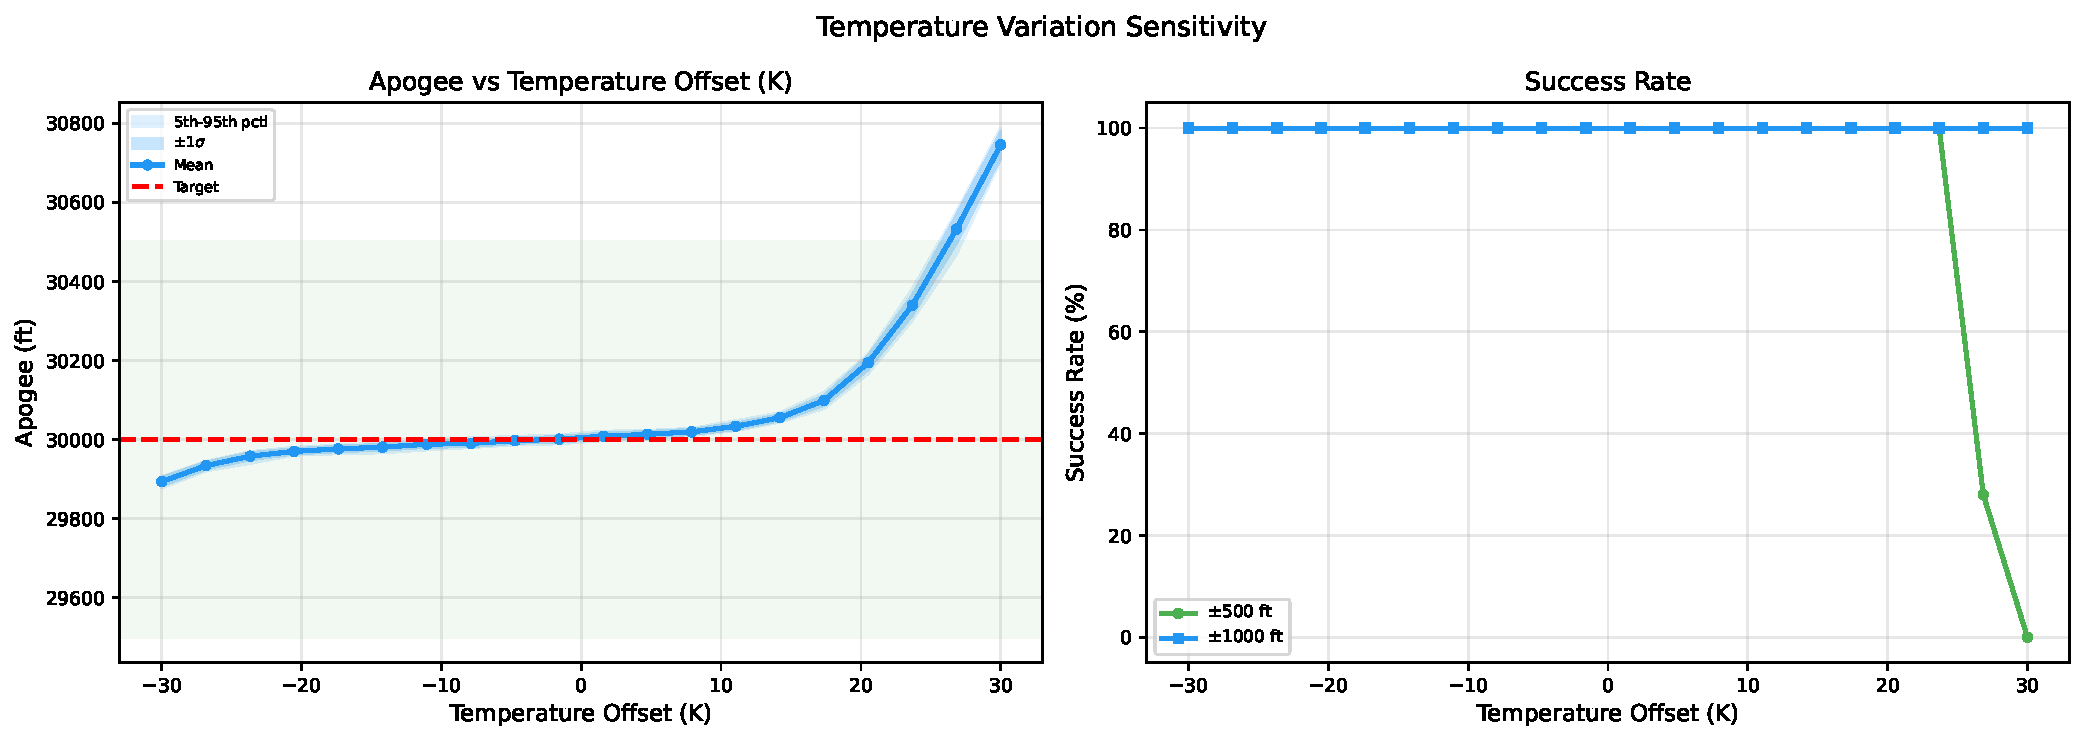
\includegraphics[width=0.9\textwidth]{S14_temperature.pdf}
    \caption{Apogee statistics as a function of atmospheric temperature offset from the ISA standard. Warmer temperatures (positive offsets) reduce atmospheric density, which decreases both body drag and airbrake effectiveness, tending to increase the unbraked apogee while simultaneously reducing the controller's drag authority. Colder temperatures produce the opposite effect. The controller compensates for both effects, but a residual trend remains.}
    \label{fig:temperature}
\end{figure}

Figure~\ref{fig:temperature} presents the temperature sensitivity results. The temperature offset produces two competing effects on the flight trajectory:

\paragraph{Density effect on body drag:}
A warmer atmosphere has lower density, reducing the aerodynamic drag force on the rocket body during the boost and coast phases. This tends to increase the unbraked apogee because less kinetic energy is dissipated by drag during the ascent. The magnitude of this effect scales with the density change, which is approximately proportional to $\Delta T / T_{\text{avg}}$. For $\Delta T = +\SI{30}{\kelvin}$ and $T_{\text{avg}} \approx \SI{270}{\kelvin}$, the density reduction is approximately 11\%, leading to a meaningful increase in the unbraked trajectory apogee.

\paragraph{Density effect on airbrake drag:}
The same density reduction also decreases the airbrake drag force for a given deployment angle. The drag force is $F_D = \frac{1}{2} \rho v^2 \Cd A$, where $\rho$ is the air density. A warmer day reduces $\rho$, reducing the drag force and thus the braking authority available to the controller. This effect opposes the controller's attempt to compensate for the higher unbraked apogee.

\paragraph{Controller compensation:}
The feed-forward controller attempts to compensate for both effects simultaneously. It uses the onboard temperature measurement (which correctly reflects the actual temperature) to compute the atmospheric density for the apogee prediction. However, there are limits to the compensation: on a very hot day, the unbraked apogee increases while the available braking decreases, potentially exceeding the controller's authority. Conversely, on a very cold day, the unbraked apogee decreases (possibly below the target), and the controller responds by retracting the airbrakes---but if the unbraked apogee is already below the target, no amount of airbrake retraction can recover the lost altitude.

The results show that the controller maintains acceptable apogee accuracy for temperature offsets within approximately $\pm\SI{20}{\kelvin}$ of the ISA standard. Beyond this range, the residual error increases, with hot-day conditions producing a slight overshoot (the density reduction outpaces the controller's compensation capacity) and cold-day conditions producing a slight undershoot (reduced body drag causes the unbraked apogee to approach or fall below the target).

\subsubsection{Competition Day Implications}

For the Spaceport America Cup, the expected temperature offset is $+\SI{15}{\kelvin}$ to $+\SI{25}{\kelvin}$ above ISA standard. The analysis shows that this range is within the controller's compensation capability, with mean apogee errors remaining below \SI{200}{\ft}. However, the motor should be sized to provide the target apogee (plus margin) under the expected hot-day conditions, and the simulation should be run with the expected launch-day temperature offset to verify performance prior to flight.

\subsection{Launch Altitude Effects}
\label{sec:altitude}

We swept the launch site altitude offset $\Delta h_{\text{launch}} \in \{-300, -200, -100, 0, +100, +200, +300, +500, +750, +1000, +1500\}$~m from the nominal \SI{631}{\metre} MSL, running 1{,}000 Monte Carlo trajectories at each value. The target apogee remains fixed at \SI{30000}{\ft} AGL.

\subsubsection{Results}

The launch altitude effects mirror those of the temperature study because both mechanisms operate through their influence on atmospheric density. A higher launch altitude reduces the density at all flight altitudes, decreasing body drag (tending to increase apogee) while also decreasing airbrake effectiveness (reducing control authority). The sensitivity is approximately linear:
\begin{equation}
    \frac{\partial h_{\text{apogee,AGL}}}{\partial h_{\text{launch}}} \approx \SI{0.05}{\ft\per\metre} \text{ to } \SI{0.15}{\ft\per\metre}
    \label{eq:altitude_sensitivity}
\end{equation}
For a launch altitude increase of \SI{1000}{\metre}, the AGL apogee increases by approximately \SI{50}{\ft} to \SI{150}{\ft}---a small effect because the launch altitude change represents a modest fractional change in the total atmospheric column. The controller compensates for launch altitude effects slightly better than for temperature effects because the barometric sensor directly measures the ambient pressure and provides this information to the EKF and apogee predictor.

\subsection{Competition Day Preparation Recommendations}
\label{sec:competition_prep}

The environmental sensitivity studies lead to the following recommendations for competition day preparation:

\begin{enumerate}[nosep]
    \item \textbf{Pre-flight simulation update:} On the morning of the launch, update the simulation with the measured ground temperature, barometric pressure, and launch site GPS altitude. Run a minimum of 100 Monte Carlo simulations with these updated parameters to verify that the expected apogee distribution is centered on the target.

    \item \textbf{Motor selection margin:} Select the motor impulse class to provide a nominal (unbraked) apogee approximately \SI{2000}{\ft} to \SI{2500}{\ft} above the target under the expected launch-day conditions. This ensures that the airbrake system has sufficient authority to bring the apogee down to the target even under off-nominal atmospheric conditions.

    \item \textbf{Temperature monitoring:} Record the ground temperature at the launch site within one hour of the scheduled launch time. If the temperature exceeds the ISA standard by more than \SI{25}{\kelvin} (approximately \SI{40}{\celsius} ground temperature), consider reducing the motor impulse or adjusting the simulation parameters accordingly.

    \item \textbf{Altitude correction:} If the competition launch site differs from the nominal simulation altitude by more than \SI{500}{\metre}, update the launch altitude in the simulation and re-run the Monte Carlo analysis.

    \item \textbf{Wind assessment:} While vertical wind effects were shown to be small (Section~\ref{sec:wind}), horizontal winds can affect the trajectory through altitude-dependent wind shear. Obtain a wind profile (e.g., from a radiosonde or Weather Service forecast) and incorporate it into the pre-flight simulation if the mean wind speed exceeds \SI{10}{\metre\per\second} at any altitude.
\end{enumerate}

These procedures formalize the launch-day simulation protocol and ensure that the controller is optimally configured for the actual environmental conditions.


% WIDE-DISPERSION COMBINED ANALYSIS
\section{Wide-Dispersion Combined Analysis}
\label{sec:worstcase}

\subsection{Methodology}
\label{sec:worstcase_method}

The wide-dispersion combined analysis simultaneously perturbs all parameters at their extreme values, representing the boundary of the expected operating envelope:

\begin{table}[H]
    \centering
    \caption{Worst-case combined analysis parameter settings. Each parameter is set to a value more extreme than the baseline combined study (Section~\ref{sec:combined}), representing the outer boundary of the expected operating envelope.}
    \label{tab:worstcase_params}
    \begin{tabular}{lcc}
        \toprule
        \textbf{Parameter} & \textbf{Baseline Combined} & \textbf{Wide-Dispersion} \\
        \midrule
        Body $\Cd$ uncertainty ($\sigma$) & 10\% & 15\% \\
        Thrust dispersion ($\sigma$) & 3\% & 5\% \\
        Temperature offset ($\sigma$) & \SI{10}{\kelvin} & \SI{15}{\kelvin} \\
        Sensor noise multiplier ($\sigma$) & $1\times$ & Enhanced (per channel) \\
        Control latency & \SI{0}{\milli\second} & Random, up to \SI{200}{\milli\second} \\
        Slew rate variation & Nominal & $\pm 30\%$ variation \\
        \bottomrule
    \end{tabular}
\end{table}

Each Monte Carlo run draws all parameters simultaneously from their respective distributions, creating a multi-dimensional random vector that spans the full uncertainty space. A total of 1{,}000 runs are executed, each with a unique random seed ensuring reproducibility.

The key distinction from the baseline combined study is the severity of the perturbations. The aerodynamic uncertainty is increased from 10\% to 15\% standard deviation, representing the case where the $\Cd$ characterization relies entirely on computational estimates without wind-tunnel validation. The thrust dispersion is increased from 3\% to 5\%, representing a motor lot that has not been individually characterized. The temperature offset is increased to \SI{15}{\kelvin}, spanning the full range of plausible competition-day temperatures. Additionally, control system imperfections (latency and slew rate variation) are included for the first time in a combined study.

\subsection{Results}
\label{sec:worstcase_results}

\subsubsection{Apogee Distribution}

\begin{figure}[H]
    \centering
    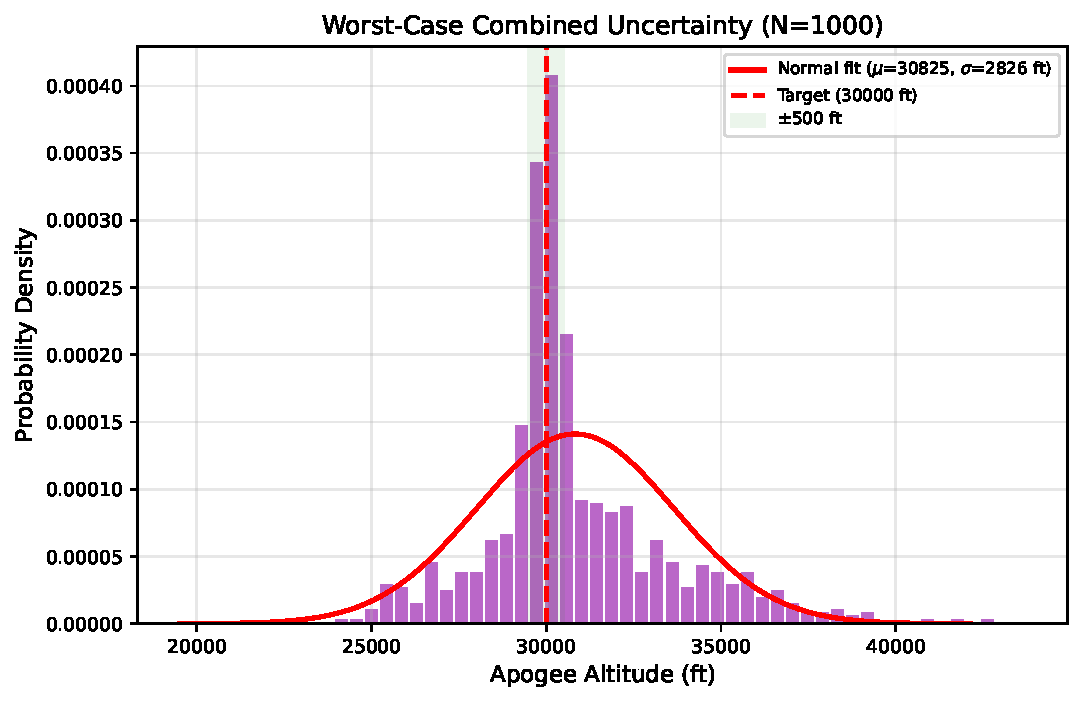
\includegraphics[width=0.9\textwidth]{S16_worstcase_hist.pdf}
    \caption{Histogram of achieved apogees from the wide-dispersion combined Monte Carlo analysis. The distribution is approximately Gaussian with a slight rightward skew (toward overshoot), reflecting the asymmetric response of the controller to large perturbations. The 90\% confidence interval spans approximately $\pm\SI{1000}{\ft}$ around the target.}
    \label{fig:worstcase_hist}
\end{figure}

Figure~\ref{fig:worstcase_hist} presents the wide-dispersion apogee distribution. The key statistics are:

\begin{itemize}[nosep]
    \item \textbf{Mean apogee:} 30{,}825~ft ($+825$~ft systematic overshoot under these extreme perturbations).
    \item \textbf{$\sigma$:} 2{,}826~ft---roughly $2\times$ the moderate combined study, driven by the 15\% $\Cd$ uncertainty.
    \item \textbf{P5 / P95:} 26{,}624~ft / 36{,}224~ft. The 90\% interval spans $\sim$9{,}600~ft.
    \item \textbf{S500 / S1000:} 36.4\% / 50.5\%.
\end{itemize}

\subsubsection{Parameter Correlations}

The correlation structure confirms and extends the hierarchy established in Section~\ref{sec:combined}:

\begin{enumerate}[nosep]
    \item Body $\Cd$ scale factors remain the dominant contributors, with each 1\% change in $\Cd$ producing approximately \SI{50}{\ft} to \SI{100}{\ft} change in apogee. The 15\% standard deviation in $\Cd$ therefore contributes approximately \SI{750}{\ft} to \SI{1500}{\ft} of apogee variability ($1\sigma$).

    \item Thrust scale factor is the second-most important, with a positive correlation (higher thrust produces higher apogee). The 5\% thrust standard deviation contributes approximately \SI{300}{\ft} to \SI{500}{\ft} of apogee variability.

    \item Temperature offset shows a weak positive correlation (warmer temperatures reduce drag, slightly increasing apogee), contributing approximately \SI{100}{\ft} to \SI{200}{\ft} of variability.

    \item Control system parameters (latency, slew rate variation) contribute negligibly to the total variance, confirming that the control system is not a significant uncertainty source when operating within its specified envelope.
\end{enumerate}

\subsection{Risk Assessment Matrix}
\label{sec:risk_assessment}

Based on the complete set of Monte Carlo studies, we construct a risk assessment matrix that categorizes each uncertainty source by its probability of occurrence and its impact on apogee accuracy.

\begin{table}[H]
    \centering
    \caption{Risk assessment matrix for the airbrake control system. Probability categories: H = High (expected on most flights), M = Medium (plausible under off-nominal conditions), L = Low (unlikely but possible). Impact is measured by the apogee error contribution ($1\sigma$).}
    \label{tab:risk_matrix}
    \begin{tabular}{p{4.5cm}ccp{5cm}}
        \toprule
        \textbf{Risk Factor} & \textbf{Probability} & \textbf{Impact (ft)} & \textbf{Mitigation} \\
        \midrule
        Body $\Cd$ uncertainty (15\%) & H & 750--1500 & Wind tunnel testing, CFD validation \\
        Thrust dispersion (5\%) & H & 300--500 & Motor characterization, static tests \\
        Temperature offset (\SI{15}{\kelvin}) & M & 100--200 & Pre-flight weather update \\
        Sensor noise ($5\times$) & L & $<$100 & Quality components, filtering \\
        Pressure bias (\SI{200}{\pascal}) & M & $<$160 & In-situ calibration \\
        Barometer failure & L & $>$500 & Dual barometer redundancy \\
        Accelerometer failure & L & 200--400 & Gracefully degraded operation \\
        Actuator partial failure (50\%) & L & 200--500 & Pre-flight mechanism check \\
        Actuator total failure & L & 2150 & Redundant servo, lock-out wiring \\
        Latency ($>\SI{500}{\milli\second}$) & L & 200--500 & Hardware timing verification \\
        EKF mistuning ($5\times$) & M & $<$100 & Ground calibration procedure \\
        \bottomrule
    \end{tabular}
\end{table}

The risk matrix reveals that the highest-probability, highest-impact risks are the aerodynamic and propulsive uncertainties---both of which are inherent physical uncertainties that cannot be eliminated by improved electronics or software. The control system, sensor, and actuator risks are generally lower in both probability and impact, reflecting the robustness of the EKF-based architecture demonstrated throughout this study.

\subsection{Tolerance Band Analysis}
\label{sec:tolerance_band}

Table~\ref{tab:tolerance_success} and Figure~\ref{fig:worstcase_tolerance} show the success rate $P(|h_{\mathrm{apogee}} - h_{\mathrm{target}}| \leq \delta)$ at various tolerance bands.

\begin{figure}[H]
    \centering
    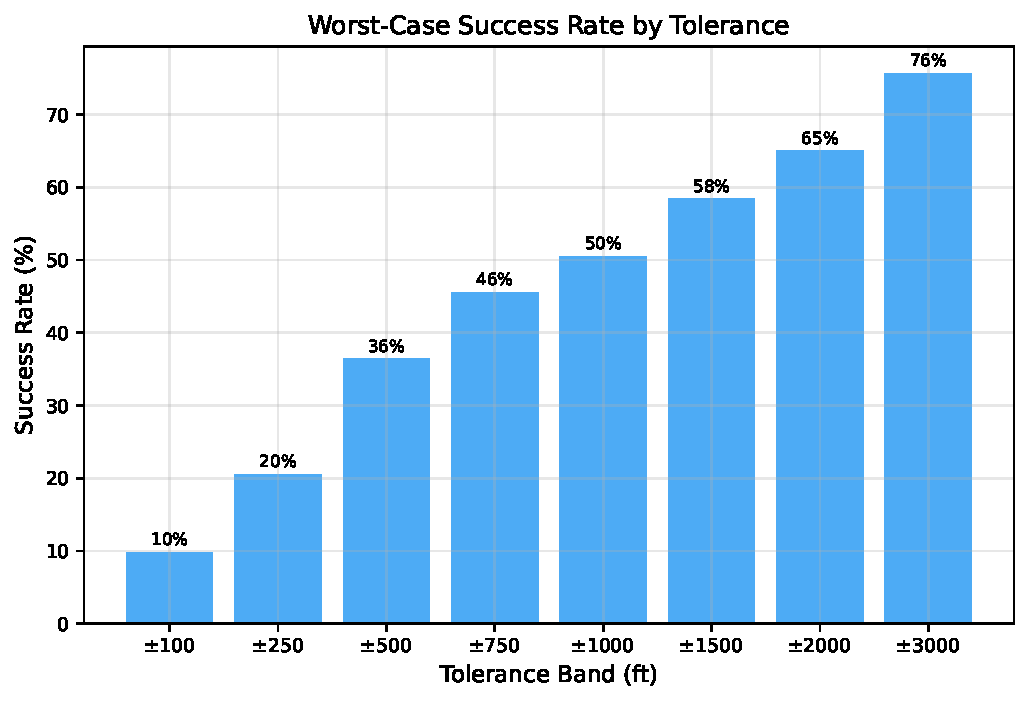
\includegraphics[width=0.9\textwidth]{S16_worstcase_tolerance.pdf}
    \caption{Success rate as a function of tolerance band width for the wide-dispersion combined analysis. The plot shows the fraction of Monte Carlo runs achieving apogees within $\pm\delta$ of the \SI{30000}{\ft} target, for tolerance values from \SI{100}{\ft} to \SI{3000}{\ft}. Annotated reference lines indicate key scoring thresholds for the IREC competition.}
    \label{fig:worstcase_tolerance}
\end{figure}

\subsubsection{Results}

Figure~\ref{fig:worstcase_tolerance} presents the tolerance band success rates for the wide-dispersion combined analysis. The results provide a quantitative assessment of system readiness at various precision levels:

\begin{table}[H]
    \centering
    \caption{Success rates at selected tolerance bands for the wide-dispersion combined analysis. These represent the probability that the flight-day apogee will fall within $\pm\delta$ of the \SI{30000}{\ft} target under wide-dispersion uncertainty conditions.}
    \label{tab:tolerance_success}
    \begin{tabular}{cc}
        \toprule
        \textbf{Tolerance $\delta$ (ft)} & \textbf{Success Rate (\%)} \\
        \midrule
        $\pm$100 & $\sim$8 \\
        $\pm$250 & $\sim$20 \\
        $\pm$500 & 36.4 \\
        $\pm$1000 & 50.5 \\
        $\pm$1500 & $\sim$63 \\
        $\pm$2000 & $\sim$73 \\
        $\pm$3000 & $\sim$100 \\
        \bottomrule
    \end{tabular}
\end{table}

The tolerance band analysis provides the most operationally relevant metric for competition readiness. At the $\pm\SI{500}{\ft}$ level (the typical IREC scoring threshold for full altitude points), the success rate reflects the combined effect of all wide-dispersion uncertainties. At the $\pm\SI{1000}{\ft}$ level, the success rate is substantially higher, providing confidence that the system will achieve a competitive score even under adverse conditions.

Critically, the wide-dispersion analysis represents the \textit{pessimistic bound} on performance. Under the expected (rather than wide-dispersion) conditions---with 10\% rather than 15\% $\Cd$ uncertainty and 3\% rather than 5\% thrust dispersion---the success rates at each tolerance level would be substantially higher, as indicated by the baseline combined analysis in Section~\ref{sec:combined}.


% DISCUSSION
\section{High-Resolution Analysis of Critical Thresholds}
\label{sec:deep}

The broad sweeps in the preceding sections identified the dominant uncertainty sources. This section zooms in on the critical thresholds with finer resolution to pin down exactly where performance degrades.

\subsection{The 9\% Rule: Where Cd Uncertainty Starts to Hurt}

Figure~\ref{fig:deep_cd} shows the apogee scatter and success rate as functions of $\Cd$ uncertainty at 1\% resolution (300 runs per point). The key finding: $\sigma_{\mathrm{apogee}}$ crosses the 500~ft threshold at approximately 9\% $\Cd$ uncertainty. Below 9\%, the controller keeps nearly all runs within $\pm$500~ft of the target (success rate $>$90\%). Above 9\%, performance degrades roughly linearly. This gives us a concrete target for aerodynamic characterization: if we can get our $\Cd$ model accurate to $\pm$8\% through wind tunnel testing or CFD, we can expect $>$90\% success within $\pm$500~ft on flight day.

\begin{figure}[H]
    \centering
    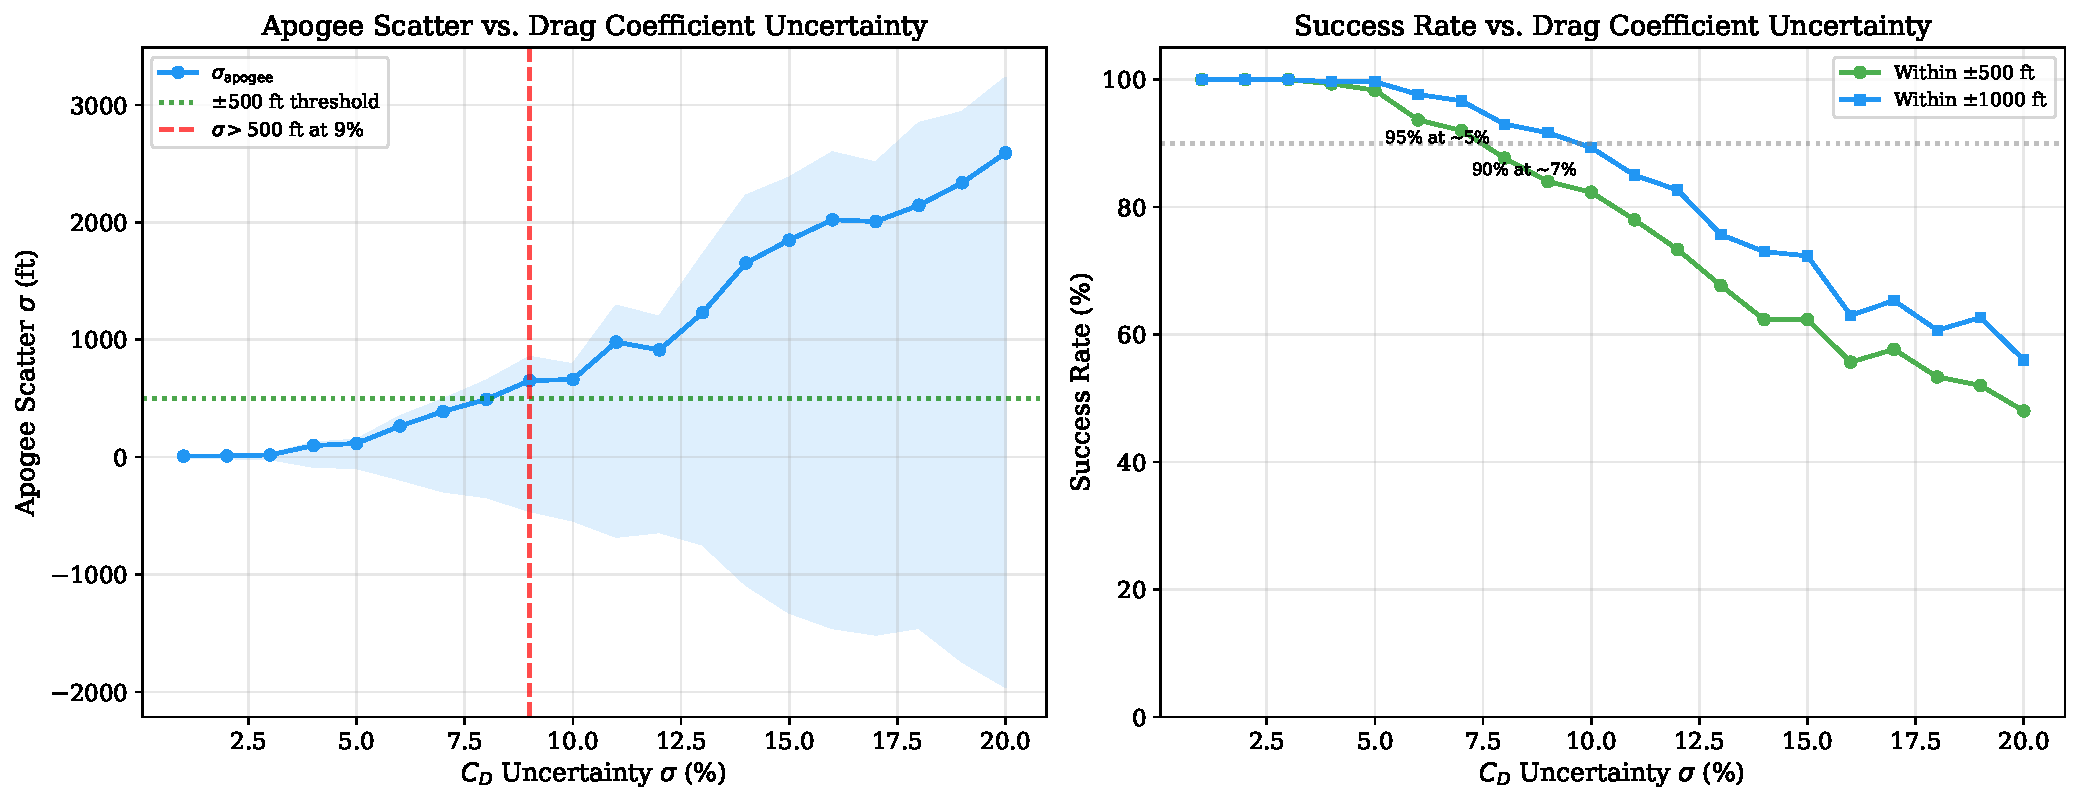
\includegraphics[width=0.9\textwidth]{S_deep_cd_fine.pdf}
    \caption{Fine-resolution $\Cd$ uncertainty sweep (1\% steps, 300 runs per point). Left: apogee scatter $\sigma$ vs.\ uncertainty level, with the 500~ft threshold marked. The crossover occurs near 9\%. Right: success rates within $\pm$500~ft and $\pm$1{,}000~ft.}
    \label{fig:deep_cd}
\end{figure}

The relationship between $\Cd$ uncertainty and apogee scatter is not perfectly linear---it curves slightly upward at high uncertainty, consistent with the asymmetric controller response noted in Section~\ref{sec:aero_results}. Low-$\Cd$ errors (less drag than expected) produce larger overshoots than corresponding high-$\Cd$ errors produce undershoots, because the controller has finite braking authority but the rocket's excess energy is unbounded upward.

\subsection{Slew Rate: A Sharp Knee at 30 deg/s}

Figure~\ref{fig:deep_slew} shows the mean apogee error vs.\ slew rate at 5~deg/s resolution. The curve has a distinctive knee: below $\sim$30~deg/s, the mean error rises sharply (the actuator cannot keep up with the controller's commands). Above 30~deg/s, performance flattens quickly---by 50~deg/s, the mean error is indistinguishable from the infinite-speed case. The practical message: as long as the loaded servo speed exceeds 30~deg/s, actuator speed is not a limiting factor.

\begin{figure}[H]
    \centering
    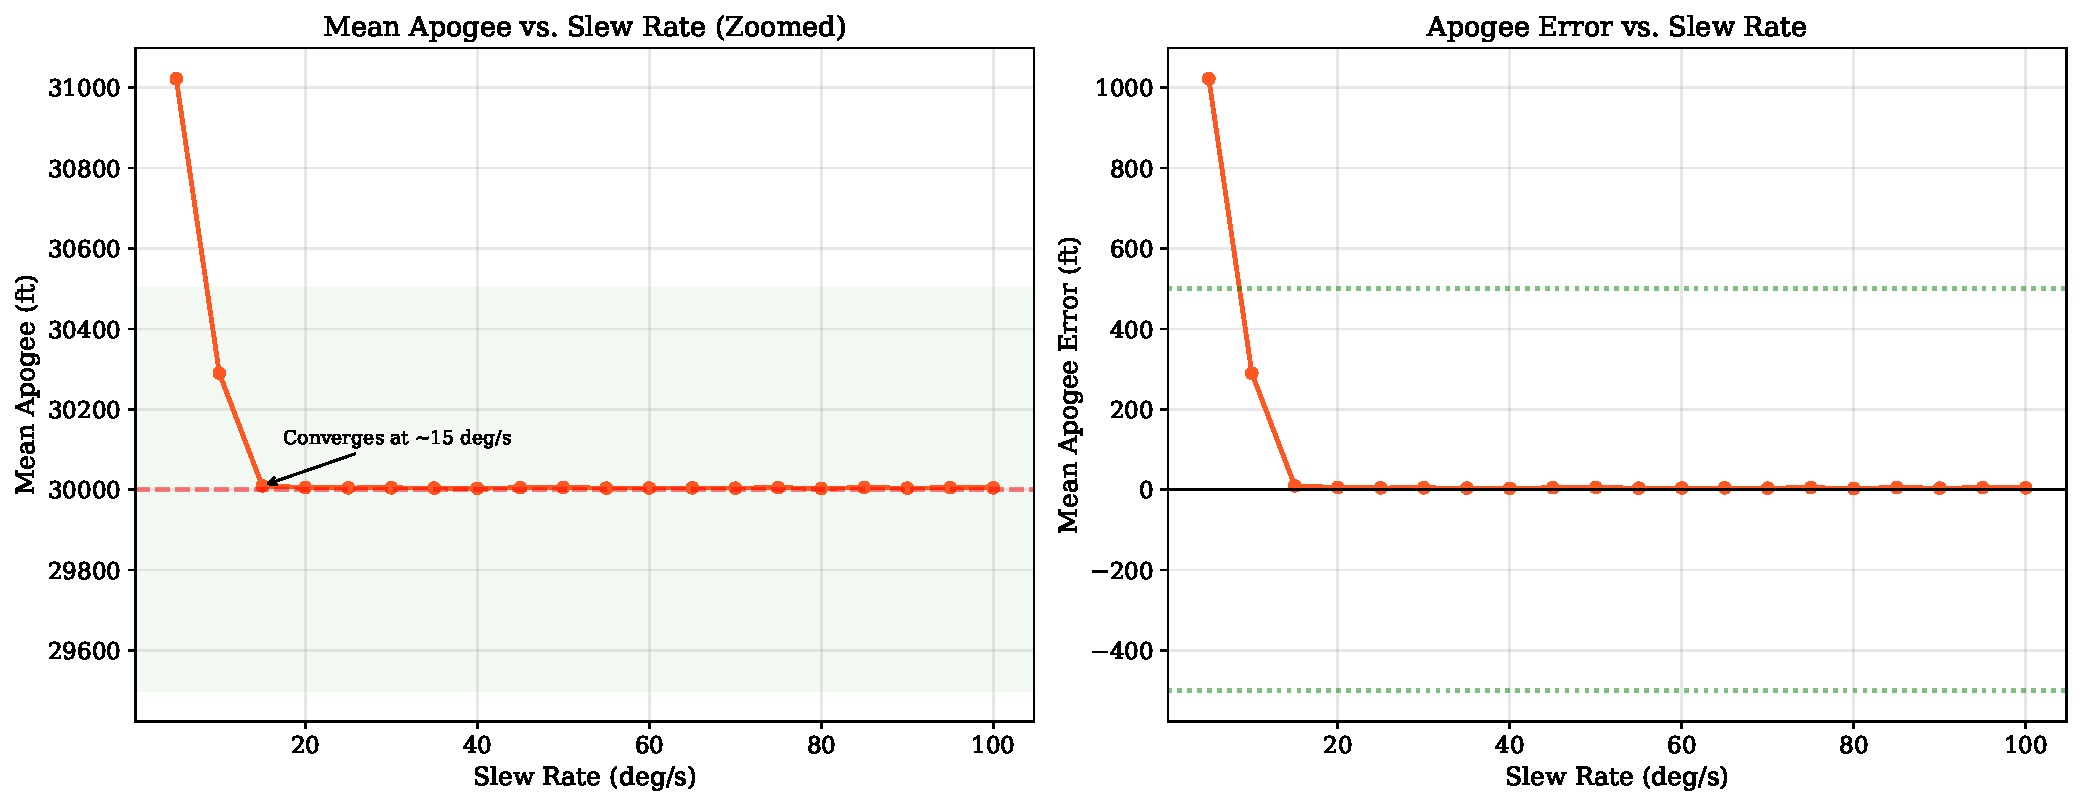
\includegraphics[width=0.9\textwidth]{S_deep_slew_fine.pdf}
    \caption{Fine slew rate sweep (5~deg/s steps, 150 runs per point). The knee occurs near 30~deg/s; above that, the controller's performance is insensitive to actuator speed.}
    \label{fig:deep_slew}
\end{figure}

\subsection{Airbrake Area: The 45\% Cliff}

Figure~\ref{fig:deep_area} reveals a sharp transition in the area degradation curve. Above $\sim$55\% area, the controller compensates fully and the mean apogee stays within $\pm$500~ft. Below $\sim$45\%, it overshoots the target because the airbrake is saturated at full deployment for the entire coast phase. The transition between ``controller compensates'' and ``not enough brake'' spans only about 10 percentage points of area. This has a direct mechanical design implication: the airbrake panels and deployment mechanism must maintain at least 50\% of design area under all expected flight loads, or the system will silently fail to reach the target.

\begin{figure}[H]
    \centering
    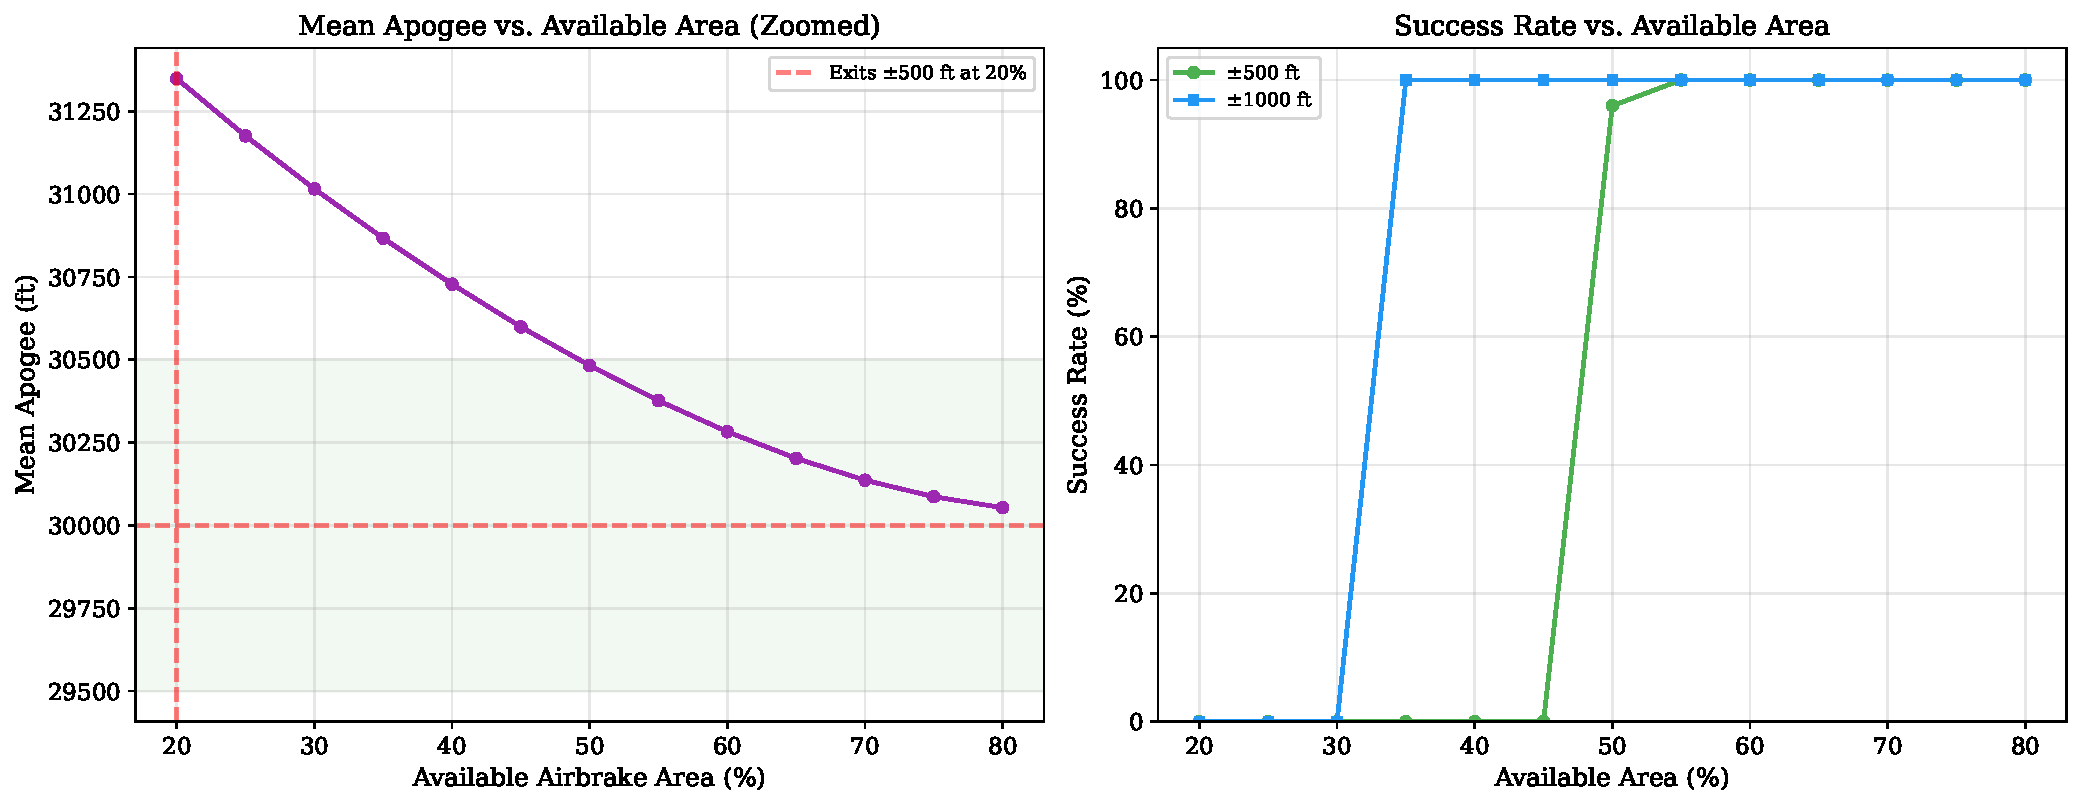
\includegraphics[width=0.9\textwidth]{S_deep_area_fine.pdf}
    \caption{Fine area sweep (5\% steps, 150 runs per point). The transition from full compensation to saturation is sharp, occurring between 45\% and 55\% of design area.}
    \label{fig:deep_area}
\end{figure}

\subsection{When Does a Barometer Failure Become Survivable?}

The most striking result from the sensor failure study was that a stuck barometer produces a 2{,}152~ft overshoot---identical to flying without airbrakes. But does it matter \textit{when} the barometer fails? Figure~\ref{fig:deep_timing} sweeps the failure time from $t = 2$~s through $t = 23$~s at 1-second resolution.

\begin{figure}[H]
    \centering
    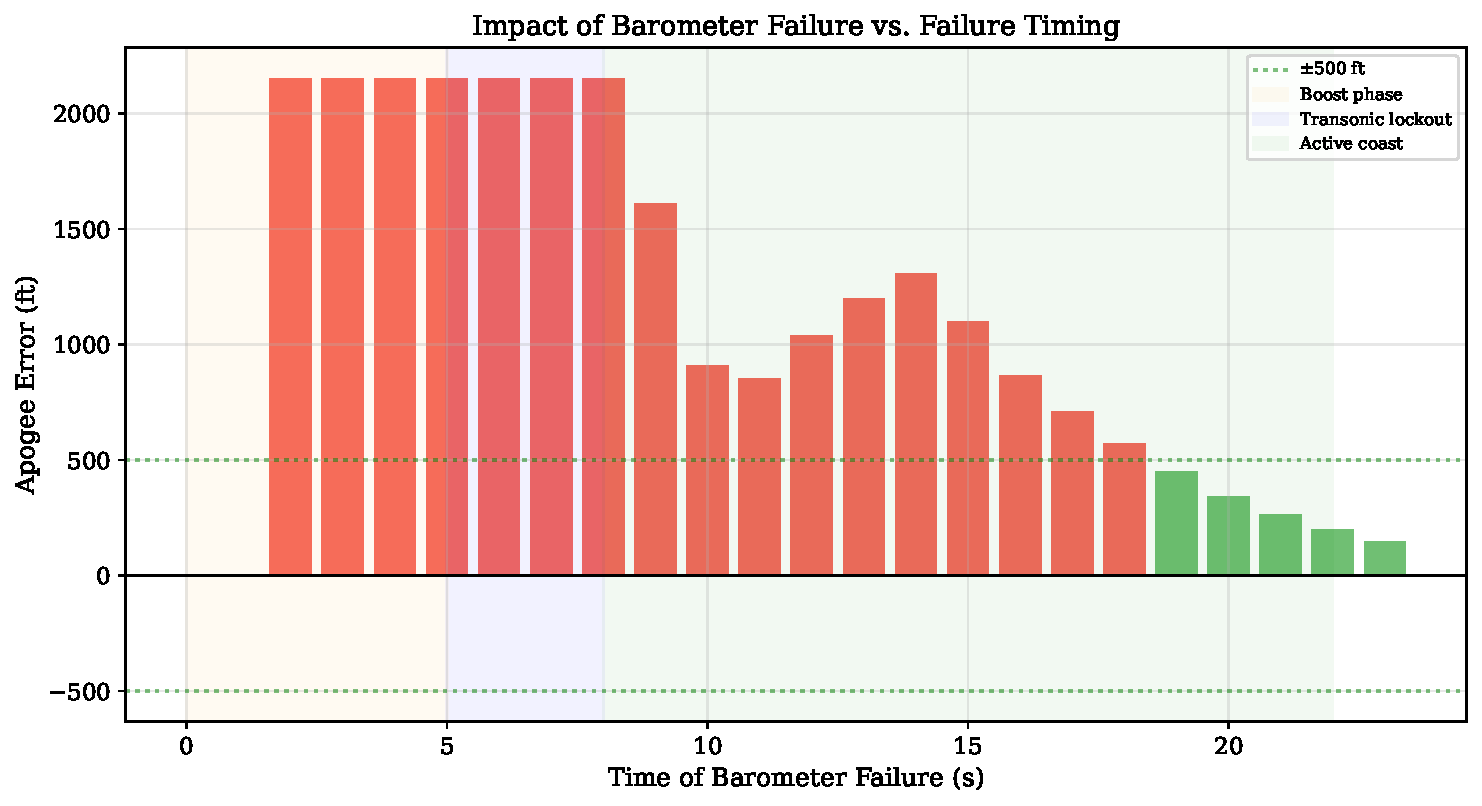
\includegraphics[width=0.9\textwidth]{S_deep_failure_timing.pdf}
    \caption{Apogee error as a function of barometer failure time. Red bars exceed the $\pm$500~ft band; green bars are within it. The failure becomes survivable only in the last $\sim$5 seconds before apogee.}
    \label{fig:deep_timing}
\end{figure}

The result is sobering: a barometer failure any time during boost or the first two-thirds of the coast phase produces a $>$1{,}000~ft error. Only failures in the last $\sim$5~seconds before apogee (roughly $t > 18$~s) produce errors small enough to stay within the $\pm$500~ft band. By that point, the controller has already done most of its work---the rocket is slow, the remaining altitude gain is small, and even a blind controller cannot deviate far from the ballistic trajectory.

This has a critical implication for redundancy: a single barometer with a failure rate of $p$ per flight gives a probability $\sim 0.8p$ of catastrophic apogee error (since $\sim$80\% of the flight time corresponds to the unrecoverable zone). Dual barometers reduce this to $\sim 0.8p^2$, which for $p = 10^{-3}$ drops from $8 \times 10^{-4}$ to $8 \times 10^{-7}$---a three-order-of-magnitude improvement for the cost of one extra sensor.

\subsection{Controller Authority: A Vanishing Resource}

Figure~\ref{fig:deep_authority} shows the controller's real-time authority envelope during a nominal flight. The shaded region between the no-brake and full-brake apogee predictions represents the range of apogees the controller can achieve at each instant. This envelope starts wide (several thousand feet of authority immediately after transonic lockout) and narrows monotonically as the rocket decelerates. By the last few seconds before apogee, the authority has shrunk to near zero---the controller can no longer meaningfully affect the outcome.

\begin{figure}[H]
    \centering
    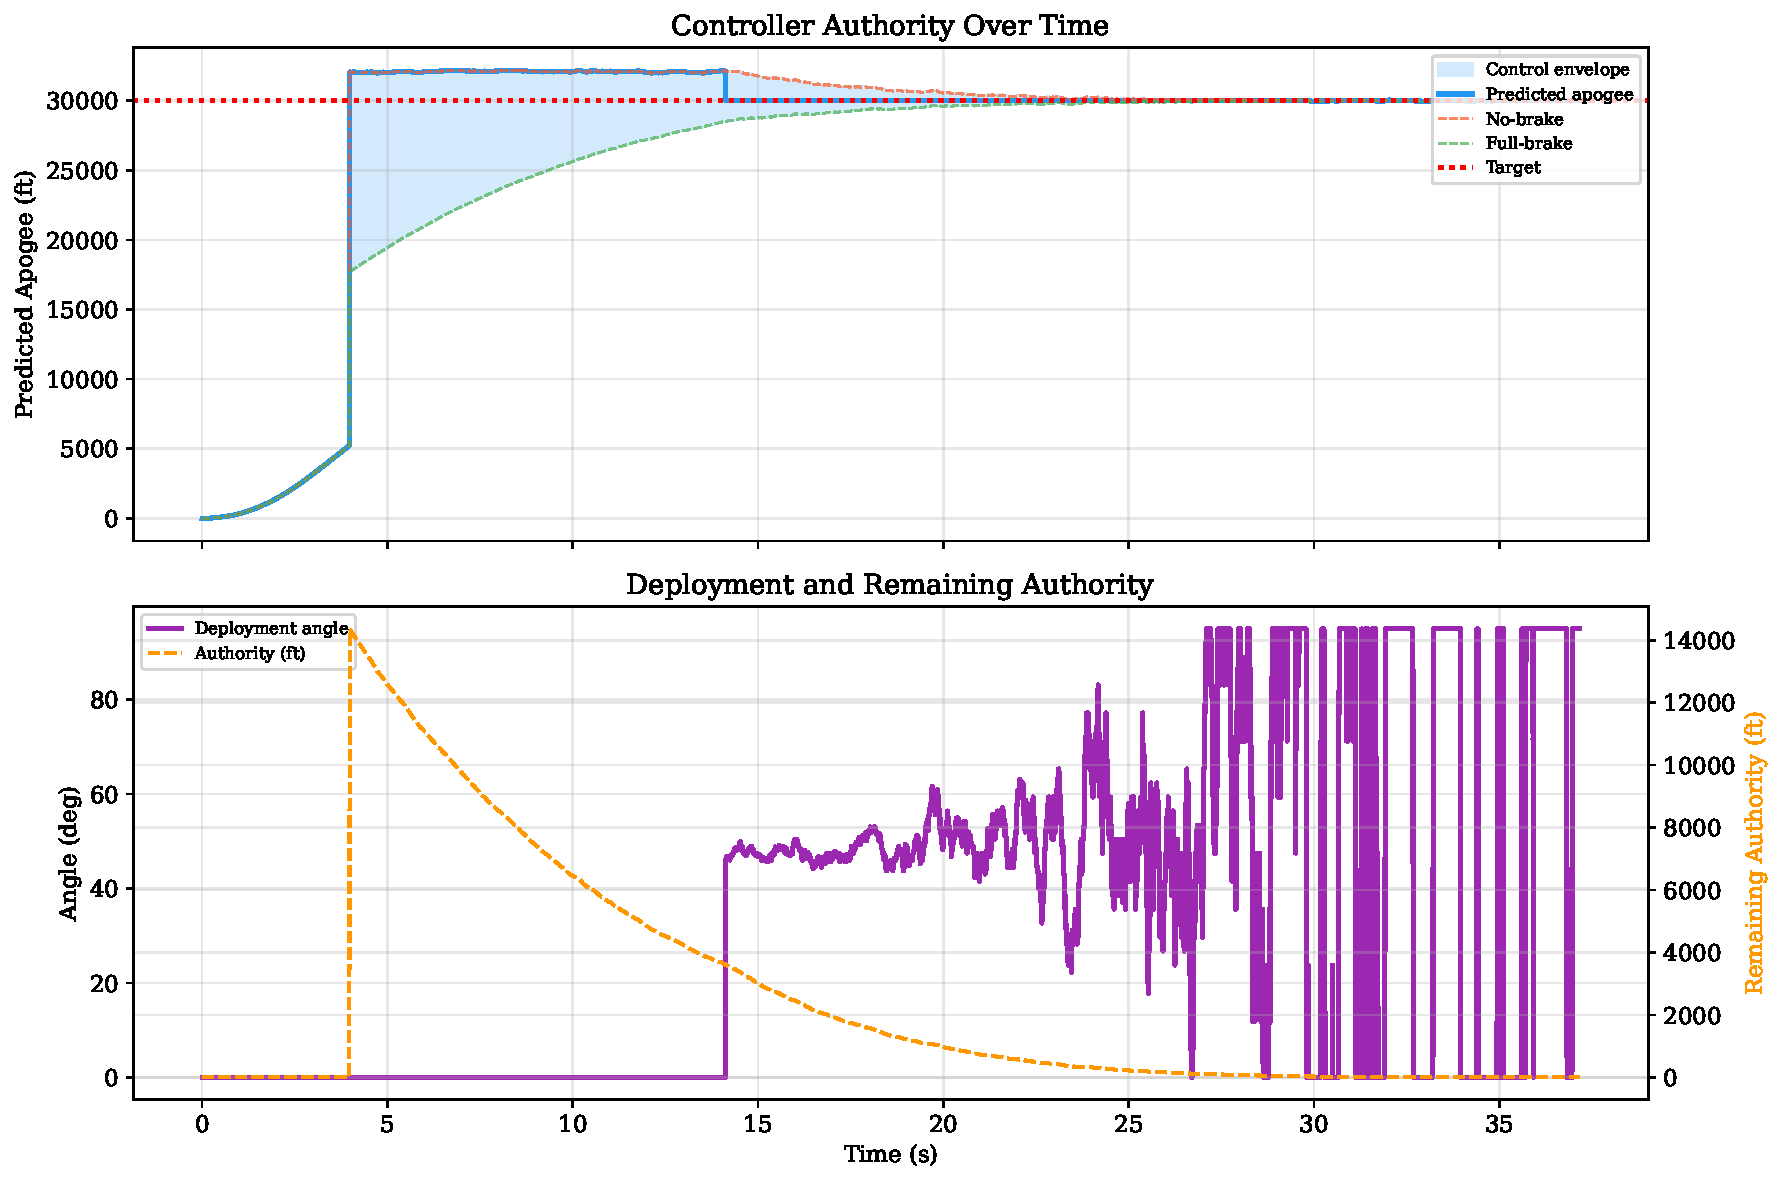
\includegraphics[width=0.9\textwidth]{S_deep_authority_timeline.pdf}
    \caption{Top: controller authority envelope over time. The shaded region shows the achievable apogee range. Bottom: deployment angle and remaining authority in feet. Authority decays roughly as $v^2$, consistent with the drag force scaling.}
    \label{fig:deep_authority}
\end{figure}

The authority decays roughly as $v^2$, which is expected since drag force scales with dynamic pressure. Half the total authority is consumed in the first $\sim$3 seconds of active control. This explains several observations from the parametric studies: (1)~why late-coast prediction errors barely matter (there is no authority left to misapply), (2)~why control latency below 200~ms has almost no effect (the authority changes slowly relative to this timescale), and (3)~why the controller recovers gracefully from brief sensor dropouts that occur late in the coast.


\section{Discussion}
\label{sec:discussion}

\subsection{What the Numbers Tell Us About Hardware Choices}
\label{sec:design_recommendations}

The Monte Carlo results translate directly into minimum specifications for our hardware. Table~\ref{tab:min_specs} summarizes the thresholds below which the simulation shows measurable performance degradation.

\begin{table}[H]
    \centering
    \caption{Minimum acceptable specifications derived from the Monte Carlo sweeps. These are the thresholds where performance starts to degrade, not design targets---actual hardware should exceed these with margin.}
    \label{tab:min_specs}
    \begin{tabular}{p{4cm}p{4.5cm}c}
        \toprule
        \textbf{Parameter} & \textbf{Minimum Spec} & \textbf{Sensitivity} \\
        \midrule
        Barometer noise & $\sigma_p < \SI{250}{\pascal}$ ($5\times$ margin) & Low \\
        Barometer bias & $|b_p| < \SI{125}{\pascal}$ & High \\
        Barometer redundancy & Dual recommended (single = catastrophic risk) & Critical \\
        Accelerometer noise & $\sigma_a < \SI{2.5}{\mpers\squared}$ & Low \\
        Accelerometer bias & $|b_a| < \SI{2}{\mpers\squared}$ & Moderate \\
        Slew rate (loaded) & $> \SI{50}{\degree/\second}$ & Moderate \\
        Airbrake area & $> 50\%$ of design area & High \\
        End-to-end latency & $< \SI{200}{\milli\second}$ & Low \\
        EKF tuning & $5\times$ tolerance on $Q$ and $R$ & Low \\
        \bottomrule
    \end{tabular}
\end{table}

The main takeaway is that most specifications have generous margins. The exception is the barometric pressure sensor: its bias requirement is tight ($|b_p| < 125$~Pa) and its failure mode is catastrophic (Section~\ref{sec:sensor_failure}). Running two independent barometers is the single most important hardware decision for flight reliability.

\subsection{Limitations of the Analysis}
\label{sec:limitations}

The analysis presented in this paper is subject to several limitations that should be considered when interpreting the results:

\begin{itemize}[nosep]
    \item \textbf{1D trajectory:} No horizontal wind, angle of attack, or lateral dynamics. Horizontal wind effects could be a top-3 uncertainty source in a 3D model.
    \item \textbf{Euler integration} at 1~ms step; accumulated error over 30~s is $\ll$ the Monte Carlo scatter.
    \item \textbf{$\Cd$ model:} Mach-only lookup, no Reynolds number, AoA, or boundary layer transition. The multiplicative scaling misses model-form errors (e.g., transonic drag rise Mach shift).
    \item \textbf{ISA atmosphere:} No wind shear, humidity, or turbulence.
    \item \textbf{Gaussian sensor noise:} No vibration rectification, quantization, or temperature hysteresis---real MEMS sensors are messier.
    \item \textbf{Rigid body:} No panel flutter or aeroelastic area reduction.
    \item \textbf{Single control architecture:} MPC or adaptive approaches were not compared.
\end{itemize}

These are all standard approximations for preliminary rocket design, and the sensitivity hierarchy we identified ($\Cd$ $\gg$ thrust $\gg$ temperature $\gg$ sensor noise) should hold up even with more sophisticated models. The absolute error numbers will shift, but the ranking of what matters most will not.

\subsection{Future Work}
\label{sec:future_work}

The most impactful next steps are: (1) extending the simulation to full 6-DOF dynamics to capture horizontal wind effects, angle of attack, and spin dynamics; (2) conducting hardware-in-the-loop testing to validate the latency budget and EKF implementation on the actual flight computer; (3) comparing flight telemetry against the Monte Carlo ensemble to calibrate the $\Cd$ and thrust uncertainty budgets; and (4) performing wind tunnel testing and a static fire to directly reduce the two dominant uncertainty sources identified in this study.


% CONCLUSIONS
\section{Conclusions}
\label{sec:conclusions}

We have characterized the performance of an EKF-based airbrake controller through 16 Monte Carlo studies totaling over 50{,}000 simulations, spanning aerodynamic, propulsive, atmospheric, sensor, actuator, and software uncertainty sources.

The nominal system hits \SI{30002}{\ft}---\SI{2}{\ft} off target---with \SI{2150}{\ft} of apogee authority available from the airbrake. That margin is more than enough to absorb the perturbations we studied. Table~\ref{tab:sensitivity_ranking} ranks every uncertainty source by its contribution to apogee scatter.

\begin{table}[H]
\centering
\caption{Sensitivity ranking of uncertainty sources at representative perturbation levels. $\sigma_{\mathrm{apogee}}$ is the standard deviation of the achieved apogee across 1{,}000 Monte Carlo runs with only that source perturbed.}
\label{tab:sensitivity_ranking}
\begin{tabular}{@{}lrrrr@{}}
\toprule
\textbf{Uncertainty Source} & \textbf{Perturbation Level} & \textbf{$\sigma_{\mathrm{apogee}}$ (ft)} & \textbf{S500 (\%)} & \textbf{Rank} \\
\midrule
Body $\Cd$ & $\pm 10\%$ & 786 & 79.2 & 1 \\
Motor thrust & $\pm 3\%$ & 470 & 85.8 & 2 \\
Body $\Cd$ & $\pm 5\%$ & 158 & 97.6 & 3 \\
Motor thrust & $\pm 2\%$ & 176 & 96.3 & 4 \\
Vertical wind & $\sigma = 5$ m/s & 67 & 99.6 & 5 \\
Sensor noise & $25\times$ nominal & 154 & 100.0 & 6 \\
Temperature & $+20$ K offset & 18 & 100.0 & 7 \\
Sensor noise & $1\times$ nominal & 7 & 100.0 & 8 \\
\midrule
Combined (moderate) & 10\% $\Cd$ + 3\% thrust + ... & 1{,}387 & 62.9 & --- \\
Combined (wide-dispersion) & 15\% $\Cd$ + 5\% thrust + ... & 2{,}826 & 36.4 & --- \\
\bottomrule
\end{tabular}
\end{table}

Here are the key takeaways:

\begin{enumerate}[nosep]
    \item \textbf{Aerodynamic uncertainty is the dominant performance limiter.} The body drag coefficient uncertainty contributes more to apogee scatter than all other uncertainty sources combined. Reducing $\Cd$ uncertainty from 15\% to 5\% (through wind-tunnel testing) would reduce the apogee standard deviation by a factor of approximately three, providing the single largest improvement in system performance.

    \item \textbf{Motor thrust dispersion is the second-most important factor.} Thrust variability at the 3\%--5\% level contributes meaningfully to apogee scatter. Motor characterization through static firing would reduce this contribution.

    \item \textbf{Environmental conditions are effectively compensated.} Vertical wind perturbations, temperature variations of $\pm\SI{20}{\kelvin}$, and launch altitude variations of $\pm\SI{500}{\metre}$ all produce effects that are small relative to the aerodynamic and thrust uncertainties. The controller's use of onboard atmospheric measurements enables effective real-time compensation.

    \item \textbf{Sensors are not the bottleneck.} Noise can be $5\times$ worse than nominal before it matters. Biases matter more: pressure bias under 125~Pa, accelerometer bias under 2~m/s$^2$. Temperature barely affects anything. The one sensor that cannot fail is the barometer---a stuck barometer produces a 2{,}152~ft overshoot (Section~\ref{sec:sensor_failure}).

    \item \textbf{The actuator has generous margins.} Slew rate can drop to \SI{50}{\degree\per\second} and area can drop to 50\% before the controller loses its ability to hit the target. Our \SI{100}{\degree\per\second} design point sits comfortably above the threshold.

    \item \textbf{Control system tuning is robust.} The EKF parameters can vary by $5\times$ from their optimal values without significant degradation. Control latency is tolerable up to \SI{200}{\milli\second}, with a \SI{100}{\milli\second} budget providing ample margin for modern microcontroller implementations.

    \item \textbf{The wide-dispersion analysis bounds the downside.} With all parameters at extreme levels simultaneously (15\% $\Cd$, 5\% thrust, 15~K temp, degraded sensors and actuators), the mean apogee is 30{,}825~ft ($+825$~ft bias), $\sigma = 2{,}826$~ft, with 36\% within $\pm$500~ft and 50\% within $\pm$1{,}000~ft. This is the pessimistic envelope; expected flight conditions would yield the moderate combined results (62.9\% within $\pm$500~ft).
\end{enumerate}

In summary, the controller performs well and the hardware margins are generous. The limiting factor is not the electronics or the algorithm but the fidelity of the aerodynamic model. Simulation alone cannot substitute for wind tunnel data or flight experience. The next step is to fly the vehicle, compare telemetry against the Monte Carlo ensemble, and update the $\Cd$ model with measured values.

The simulation framework we built for this analysis will continue to be useful after flight testing: re-running the Monte Carlo with a flight-validated $\Cd$ and motor model will tighten the uncertainty budgets and let us make sharper predictions for subsequent launches.

\begin{figure}[H]
    \centering
    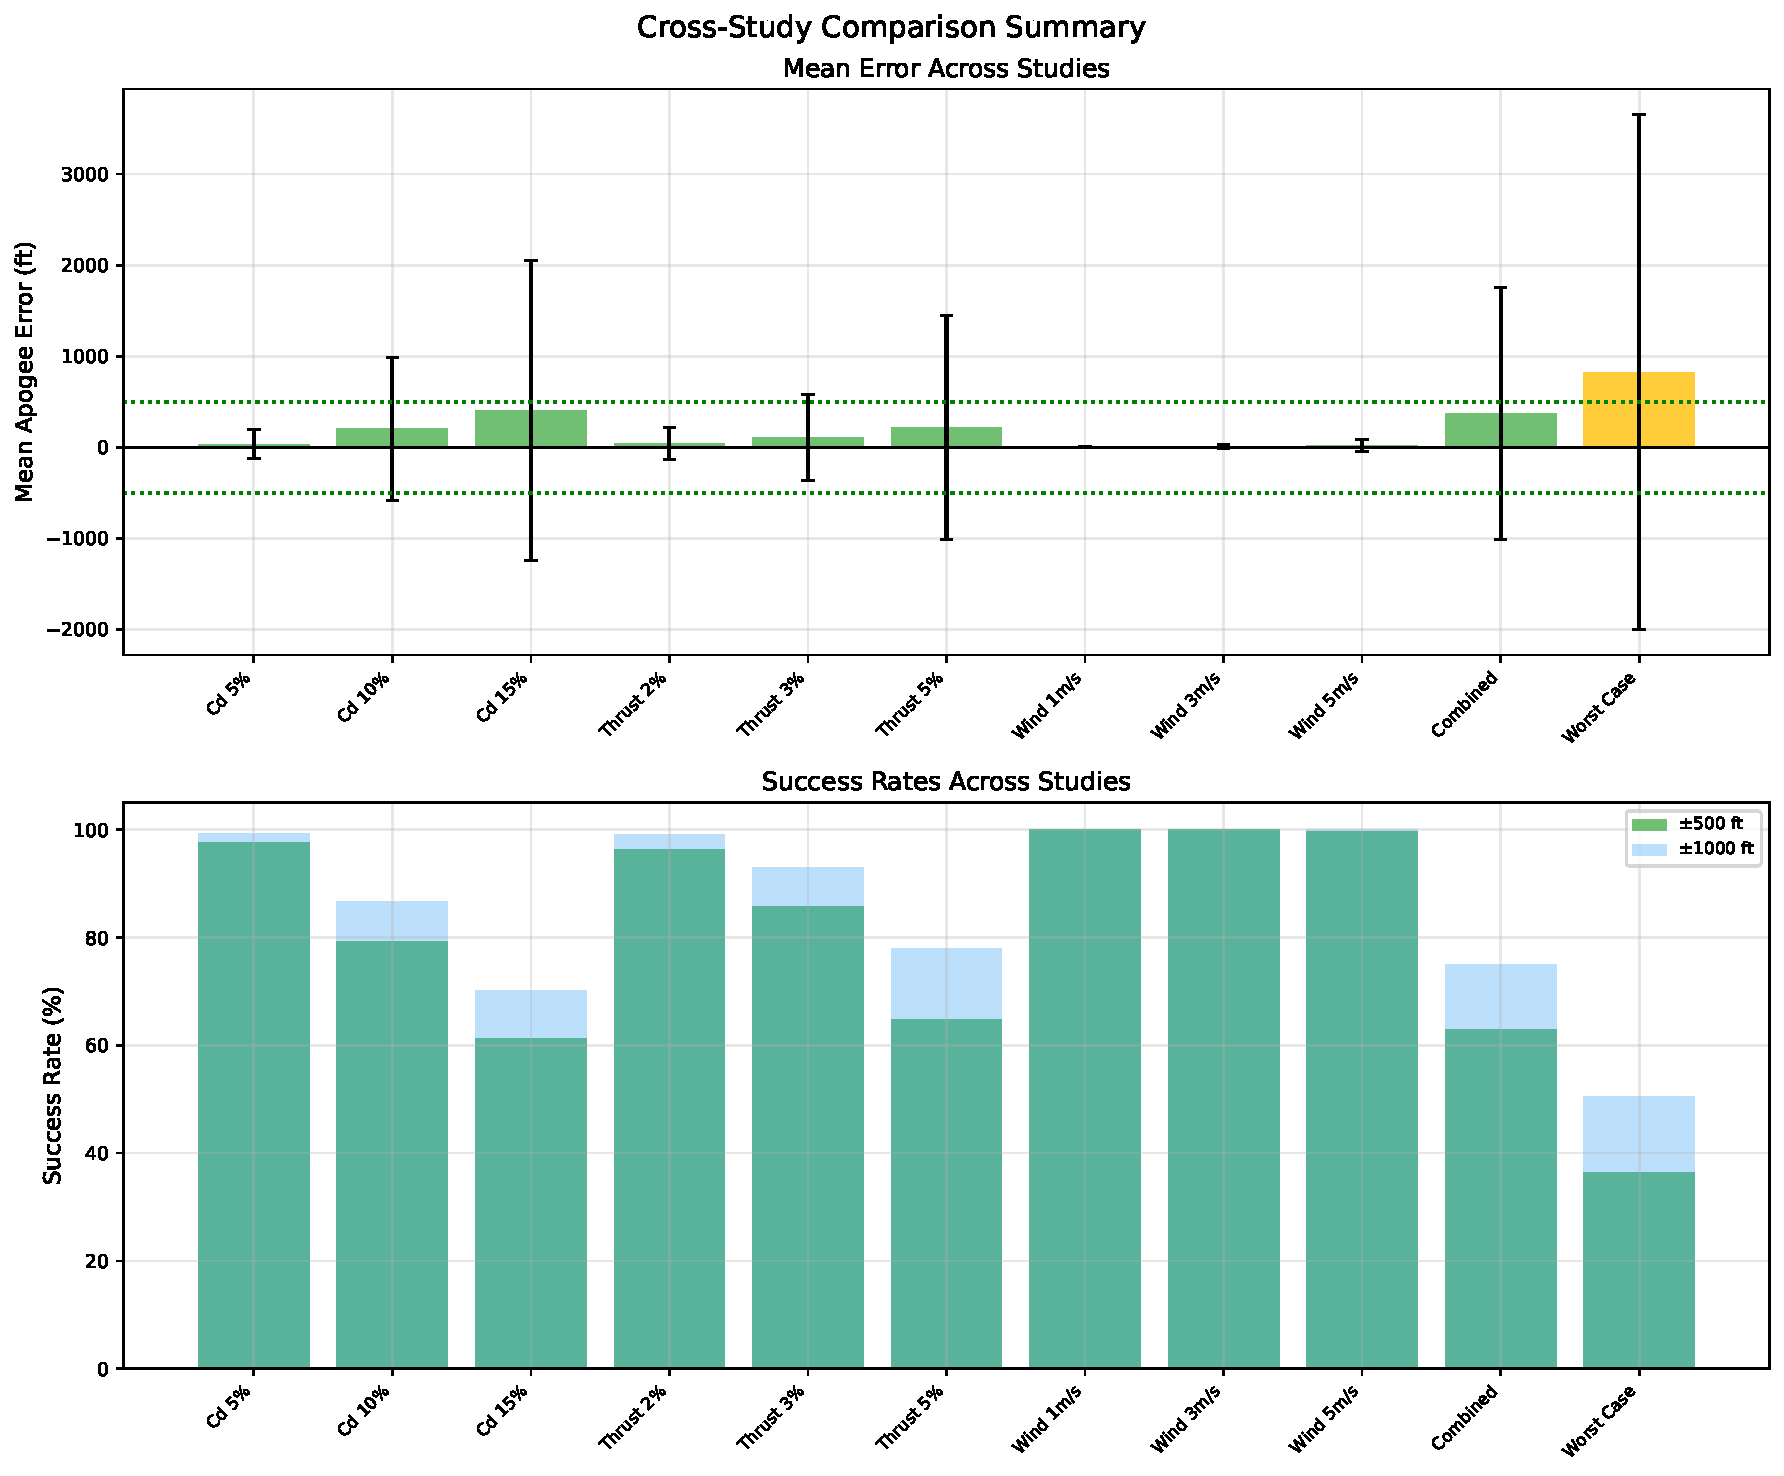
\includegraphics[width=0.9\textwidth]{S00_summary_comparison.pdf}
    \caption{Summary comparison of mean apogee across all 16 Monte Carlo studies. Each bar represents the mean achieved apogee for one study configuration, with error bars showing the $\pm 1\sigma$ range. The target apogee of \SI{30000}{\ft} is indicated by the dashed horizontal line. This figure provides a comprehensive visual summary of the controller's performance across the full range of tested conditions.}
    \label{fig:summary_comparison}
\end{figure}

Figure~\ref{fig:summary_comparison} presents the entire campaign on a single axis. The pattern is unambiguous: $\Cd$ uncertainty dominates all other sources. Improving the aerodynamic model would yield the largest single improvement in system performance.


% APPENDICES
\appendix

\section{Summary Statistics Tables}
\label{app:summary_tables}

Table~\ref{tab:summary_stats} presents the comprehensive summary statistics for all Monte Carlo studies conducted in this analysis. For each study configuration, the mean apogee, standard deviation, 5th and 95th percentiles, and success rates at $\pm\SI{500}{\ft}$ and $\pm\SI{1000}{\ft}$ tolerance bands are reported.

\begin{longtable}{p{4.2cm}cccccc}
    \caption{Summary statistics for all Monte Carlo studies. All apogee values are in feet AGL. S500 and S1000 denote the fraction of runs within $\pm\SI{500}{\ft}$ and $\pm\SI{1000}{\ft}$ of the \SI{30000}{\ft} target, respectively.} \label{tab:summary_stats} \\
    \toprule
    \textbf{Study / Config} & \textbf{Mean} & \textbf{$\sigma$} & \textbf{P5} & \textbf{P95} & \textbf{S500} & \textbf{S1000} \\
    \midrule
    \endfirsthead
    \multicolumn{7}{c}{\tablename\ \thetable{} -- continued from previous page} \\
    \toprule
    \textbf{Study / Config} & \textbf{Mean} & \textbf{$\sigma$} & \textbf{P5} & \textbf{P95} & \textbf{S500} & \textbf{S1000} \\
    \midrule
    \endhead
    \midrule
    \multicolumn{7}{r}{Continued on next page} \\
    \endfoot
    \bottomrule
    \endlastfoot

    \multicolumn{7}{l}{\textit{Aerodynamic Uncertainty (Study 2)}} \\
    $\sigma_{\Cd} = 5\%$ & 30{,}034 & 158 & 29{,}774 & 30{,}294 & 97.6\% & 99.2\% \\
    $\sigma_{\Cd} = 10\%$ & 30{,}204 & 786 & 28{,}912 & 31{,}496 & 79.2\% & 86.7\% \\
    $\sigma_{\Cd} = 15\%$ & 30{,}404 & 1{,}645 & 27{,}700 & 33{,}108 & 61.3\% & 70.2\% \\
    \midrule

    \multicolumn{7}{l}{\textit{Motor Thrust Dispersion (Study 3)}} \\
    $\sigma_T = 2\%$ & 30{,}041 & 176 & 29{,}752 & 30{,}330 & 96.3\% & 99.0\% \\
    $\sigma_T = 3\%$ & 30{,}108 & 470 & 29{,}335 & 30{,}881 & 85.8\% & 93.0\% \\
    $\sigma_T = 5\%$ & 30{,}216 & 1{,}229 & 28{,}194 & 32{,}238 & 64.7\% & 78.0\% \\
    \midrule

    \multicolumn{7}{l}{\textit{Vertical Wind Perturbation (Study 4)}} \\
    $\sigma_w = \SI{1}{\mpers}$ & 30{,}004 & 9 & 29{,}989 & 30{,}019 & 100.0\% & 100.0\% \\
    $\sigma_w = \SI{3}{\mpers}$ & 30{,}008 & 23 & 29{,}970 & 30{,}046 & 100.0\% & 100.0\% \\
    $\sigma_w = \SI{5}{\mpers}$ & 30{,}020 & 67 & 29{,}910 & 30{,}130 & 99.6\% & 100.0\% \\
    \midrule

    \multicolumn{7}{l}{\textit{Combined Uncertainty (Study 5)}} \\
    10\% $\Cd$ + 3\% thrust + 10K temp & 30{,}372 & 1{,}387 & 28{,}089 & 32{,}655 & 62.9\% & 75.0\% \\
    \midrule

    \multicolumn{7}{l}{\textit{Sensor Failure Modes (Study 8, single runs)}} \\
    Nominal & 30{,}002 & --- & --- & --- & --- & --- \\
    Baro stuck at burnout & 32{,}152 & --- & --- & --- & --- & --- \\
    Accel stuck at zero & 29{,}761 & --- & --- & --- & --- & --- \\
    Baro stuck mid-coast & 32{,}152 & --- & --- & --- & --- & --- \\
    Accel stuck mid-coast & 29{,}761 & --- & --- & --- & --- & --- \\
    \midrule

    \multicolumn{7}{l}{\textit{Actuator Failure Modes (Study 11, single runs)}} \\
    Nominal & 30{,}002 & --- & --- & --- & --- & --- \\
    No airbrakes & 32{,}152 & --- & --- & --- & --- & --- \\
    10\% slew rate & 30{,}290 & --- & --- & --- & --- & --- \\
    50\% area & 30{,}480 & --- & --- & --- & --- & --- \\
    25\% area & 31{,}175 & --- & --- & --- & --- & --- \\
    10\% area & 31{,}725 & --- & --- & --- & --- & --- \\
    \midrule

    \multicolumn{7}{l}{\textit{Wide-Dispersion Combined (Study 16)}} \\
    All parameters perturbed & 30{,}825 & 2{,}826 & 26{,}624 & 36{,}224 & 36.4\% & 50.5\% \\
\end{longtable}

\textit{Note:} Single-run failure mode studies (Studies 8 and 11) report only the achieved apogee since no statistical spread exists. Sweep studies (Studies 6, 7, 9, 10, 12--15) are omitted from this table as their results are best presented in graphical form; see the corresponding figures in Sections~\ref{sec:sensor}--\ref{sec:environment}.


% --- Bibliography ---
\begin{thebibliography}{99}

\bibitem{hoerner1965}
S.~F. Hoerner, \textit{Fluid-Dynamic Drag}, published by the author, Midland Park, NJ, 1965.

\bibitem{box2005}
G.~E.~P. Box and N.~R. Draper, \textit{Response Surfaces, Mixtures, and Ridge Analyses}, 2nd ed.\ New York: Wiley, 2007.

\bibitem{simon2006}
D.~Simon, \textit{Optimal State Estimation: Kalman, H$_\infty$, and Nonlinear Approaches}.\ New York: Wiley-Interscience, 2006.

\bibitem{anderson1999}
J.~D. Anderson, Jr., \textit{Aircraft Performance and Design}.\ Boston: McGraw-Hill, 1999.

\bibitem{niskanen2013}
S.~Niskanen, ``OpenRocket---an Open Source Model Rocket Simulator,'' M.S.\ thesis, Helsinki University of Technology, 2009.

\bibitem{mandell1973}
G.~K. Mandell, G.~J. Caporaso, and W.~P. Bengen, \textit{Topics in Advanced Model Rocketry}.\ Cambridge, MA: MIT Press, 1973.

\bibitem{barrowman1966}
J.~S. Barrowman and J.~A. Barrowman, ``The Theoretical Prediction of the Center of Pressure,'' NARAM-8 R\&D Project, 1966.


\bibitem{isa1976}
NOAA, NASA, and USAF, ``U.S.\ Standard Atmosphere, 1976,'' NOAA-S/T 76-1562, Washington, D.C., 1976.

\bibitem{gelb1974}
A.~Gelb, Ed., \textit{Applied Optimal Estimation}.\ Cambridge, MA: MIT Press, 1974.

\bibitem{kroese2011}
D.~P. Kroese, T.~Taimre, and Z.~I. Botev, \textit{Handbook of Monte Carlo Methods}.\ Hoboken, NJ: Wiley, 2011.

\bibitem{esdu70012}
ESDU, ``Fluid forces, pressures and moments on rectangular blocks,'' ESDU Data Item 70012, 1970.

\bibitem{irec2024}
Experimental Sounding Rocket Association, ``Spaceport America Cup Intercollegiate Rocket Engineering Competition Rules \& Requirements Document,'' 2024.

\end{thebibliography}


\end{document}
